% The methods for implementation of a behavioral, discrete-time PLL simulator and for the PLL loop filter automation and optimization will be covered here.

% \hl{Talk about how simulator is implemented:}
% \hl{Discrete simulation models of phase noise, dco etc}
% \hl{Filter optimization}
% \hl{-phase noise and lock time estimate in frequency domain}
The primary objective in this work is to obtain a very low $100\mu$W power consumption for a 2.448 GHz PLL frequency synthesizer, while achieving a carrier-to-noise ratio for the synthesized signal of $>$20 dB. Consequently, the design philosophy adhered to in this work is pursue simplicity wherever possible, in order to reduce number of sources of power draw and noise. Furthermore, this design is targeted to allow duty cycled operation to further reduce power. Thus, an all-digital architecture has been selected to enable the possibility to save the PLL state, enter an ultra-low-power sleep state, and then resume from the stored state rapidly, without requiring relocking of the PLL. 

\subsection{Proposed Architecture - ADPLL}\label{pll_arch}
	The undertaken PLL architecture is in figure \ref{fig:pll_arch}. It comprises primarily of five components: (1) counter-based phase detector for initial start up, (2) bang-bang phase detector for steady state feedback, (3) proportional-integral controller loop filter, (4) DCO implemented as a VCO plus capacitive DACs, and (5) a control and calibration engine, consisting of digital logic. The rationale for this architecture will be described in the following subsections.
	\subsubsection{Block diagram}
			\begin{figure}[htb!]
		        \centering
		        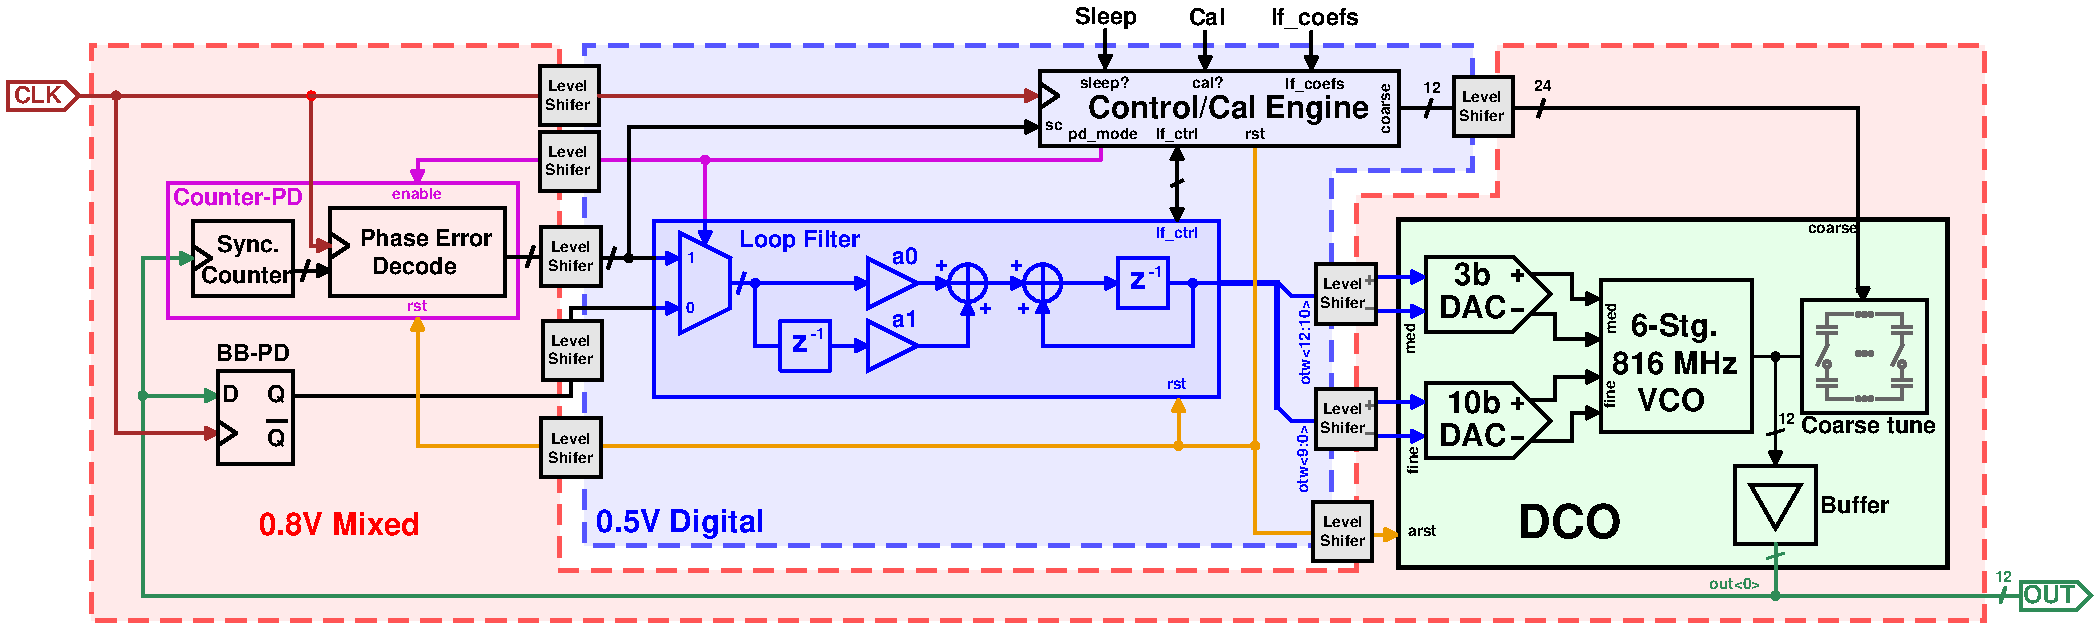
\includegraphics[width=1\textwidth, angle=0]{./figs/design/pll_master_arch_final}
			    \caption{ADPLL Architecture.}
			    \label{fig:pll_arch}
			\end{figure}

	\subsubsection{Power Saving Approach}
	Power savings have been attempted by minimization of complexity. First, the need of a divider is removed from the design by the usage of both the counter phase detector and BBPD. For initial cold start up of the PLL from an unknown state, the counter-based phase detector functions as a low-resolution replacement for a divider and linear phase detector. When near steady state, the counter-PD is disabled and replaced by BBPD feedback, which will maintain the PLL at steady state. The removal of a divider results in lower power consumption, and less noise added in-loop. The usage of only a BBPD in steady state further reduces power, as it is a minimum complexity phase detector. This is expected without significant performance degredation, as with proper optimization, BBPD PLLs can obtain comparable perform to linear charge-pump style PLLs \cite{xu_abidi_2017}. Additional power improvements are obtained in the usage of digital logic to implement the loop filter, using a simple PI-controller architecture. A divided power domain approach is used here, split between (1) 0.5V for loop filter, calibration and control logic, and (2) 0.8V for the analog portions, which constitute the DCO, in addition to the phase detectors. Multiple power domains allows for reduction of the digital logic power expenditure, while allowing for sufficient voltage for proper oscillator function. The final power saving move is implemented in a DCO based on the combination of several CDACs with a voltage controlled ring oscillator. This reduces to near zero the static curent draw associated with control of the VCO. The overall design is implemented with no static current paths, other than that associated with leakage, achieved by favoring static logic derived components throughout the PLL.

	\subsubsection{PLL Sleep Capability}
	A feature gained in the proposed all-digital architecture is the ability to abruptly save the state of the PLL digitally and place all unneeded components into an ultra low power sleep mode, and then later resume the PLL from the saved state. Figure \ref{fig:pll_sleep} demonstrate such operation, where $t_{l1}$ is the lock time from cold start, and $t_{l2}$ is the time to relock from a resume state. It is expected that slight drift in the oscillator characteristics will occur when resuming, so the relock time will likely be nonzero. However, the relock time is substantially lower than relocking from a cold state. This functionality enables the ability to rapidly duty cycle the PLL between active and sleep states. Power consumption of the PLL is reduced by a factor that is the duty cycle which it is operated; for example, 100$\mu$W nominal power consumption with 1\% duty cycle will result in 1$\mu$W average draw, which is attractive for wireless devices (particularly wake up radios).

			\begin{figure}[htb!]
			        \centering
			        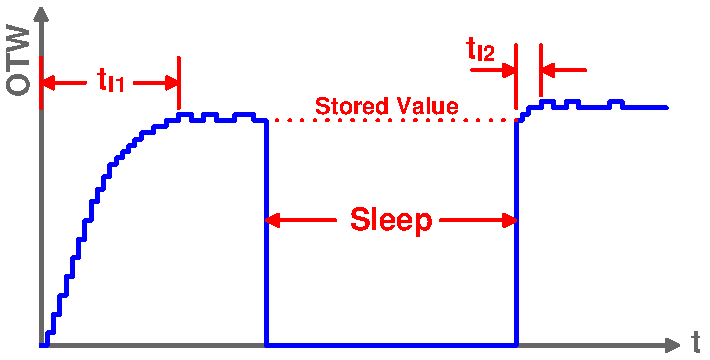
\includegraphics[width=0.6\textwidth, angle=0]{./figs/design/pll_sleep}
			    \caption{PLL sleep and resume operation.}
			    \label{fig:pll_sleep}
			\end{figure}


% \vspace{-2em}
% \begin{figure}[htb!]
% 	\center\fontfamily{\sfdefault}\selectfont
% XCircuit output "tdc_bbpll.tex" for LaTeX input from tdc_bbpll.ps
\def\putbox#1#2#3#4{\makebox[0.00000in][l]{\makebox[#1][l]{}\raisebox{\baselineskip}[0.00000in][0.00000in]{\raisebox{#2}[0.00000in][0.00000in]{\scalebox{#3}{#4}}}}}
\def\rightbox#1{\makebox[0.00000in][r]{#1}}
\def\centbox#1{\makebox[0.00000in]{#1}}
\def\topbox#1{\raisebox{-0.60\baselineskip}[0.00000in][0.00000in]{#1}}
\def\midbox#1{\raisebox{-0.20\baselineskip}[0.00000in][0.00000in]{#1}}
   \scalebox{1}{
   \normalsize
   \parbox{3.33750in}{
   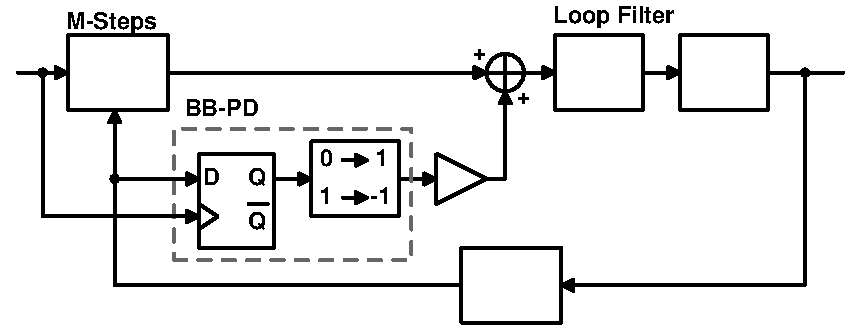
\includegraphics[scale=0.60000]{./figs/tdc_bbpll.pdf}\\
   % translate x=1412 y=528 scale 0.38
   \putbox{1.80600in}{0.70800in}{0.72}{$K_{bb}$}%
   \putbox{1.93200in}{0.14400in}{0.72}{$\div$ N}%
   \putbox{2.79600in}{0.99600in}{0.72}{DCO}%
   \putbox{2.24400in}{0.99600in}{0.72}{H$_{LF}$(z)}%
   \putbox{0.37200in}{0.99600in}{0.72}{TDC}%
   \putbox{0.03600in}{1.08600in}{0.72}{Clk}%
   \putbox{3.13200in}{1.08600in}{0.72}{Out}%
   } % close 'parbox'
   } % close 'scalebox'
   \vspace{-\baselineskip} % this is not necessary, but looks better
\fontfamily{\rmdefault}\selectfont

% 	\caption{PLL with parallel bang-bang phase detector and TDC.}
% 	\label{fig:tdc_bbpll}
% \end{figure}
	\subsubsection{Gear switching}
	The proposed digital architecture enables the ability to dynamically alter the loop filter response. This can be used to speed up lock from a cold state by using a lock time optimized filter initially, and then switch to a phase noise optimized filter after achieving initial lock. This approach is called gear switching \cite{staszewski_balsara_2007}, and is employed in this work by utilizing different loop filters for the start-up synchronous counter phase detector operation and the steady state BBPD operation.
	
	\subsubsection{Power budget}
	The below power budget was used in the design process to divide up the 100 $\mu$W allotment between the different PLL components. In order to minimize oscillator phase noise, as large of a portion was allotted to the oscillator, being 80\%. 
		\begin{table}[htb!]
			\centering
			\def\arraystretch{1.5}		
			\setlength\arrayrulewidth{0.75pt}
			\setlength{\tabcolsep}{1em} % for the horizontal padding
			\begin{tabular}{|c|c|c|c|c|}
				\hline 
				\rule[-1ex]{0pt}{2.5ex} \cellcolor{gray!40}\textbf{DCO} & \cellcolor{gray!40}\textbf{Phase detector} & \cellcolor{gray!40}\textbf{Digital (LF)}& \cellcolor{gray!40}\textbf{Other} & \cellcolor{gray!40}\textbf{SUM} \\ 
				\hline 
				\rule[-1ex]{0pt}{2.5ex} 80 $\mu$W& 10 $\mu$W &  10 $\mu$W  & 0 $ \mu$W & $\leq$ 100  $\mu$W\\ 
				\hline 
			\end{tabular} 
			\caption{Power budget for design process.}
			\label{tab:pow_budget}
		\end{table}   



	\subsubsection{Floorplan}
	The below floor plan (dimensions in microns) has been devised to meet the area requirement of $<$ 0.01 mm$^2$. The dimensions are 60$\mu$m x 85$\mu$m, with an area of 0.0051 mm$^2$. The yelow path demarcates the PLL loop signal flow. Attention was paid to separate analog (0.8V) and digital power domains (0.5V), whilst maintaining a compact area with convenient signal flow.
		\begin{figure}[htb!]
	        \centering
	        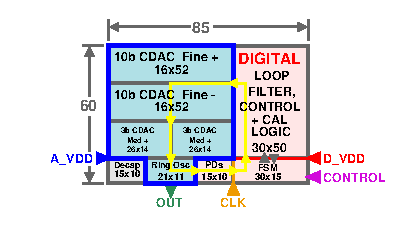
\includegraphics[width=0.75\textwidth, angle=0]{./figs/design/pll_floorplan3}
		    \caption{PLL floorplan.}
		\end{figure}

\subsubsection{Dividerless PLL}

\begin{figure}[htb!]
	\center\fontfamily{\sfdefault}\selectfont
% XCircuit output "bbpll_full_noise.tex" for LaTeX input from bbpll_full_noise.ps
\def\putbox#1#2#3#4{\makebox[0.00000in][l]{\makebox[#1][l]{}\raisebox{\baselineskip}[0.00000in][0.00000in]{\raisebox{#2}[0.00000in][0.00000in]{\scalebox{#3}{#4}}}}}
\def\rightbox#1{\makebox[0.00000in][r]{#1}}
\def\centbox#1{\makebox[0.00000in]{#1}}
\def\topbox#1{\raisebox{-0.60\baselineskip}[0.00000in][0.00000in]{#1}}
\def\midbox#1{\raisebox{-0.20\baselineskip}[0.00000in][0.00000in]{#1}}
   \scalebox{1}{
   \normalsize
   \parbox{5.50000in}{
   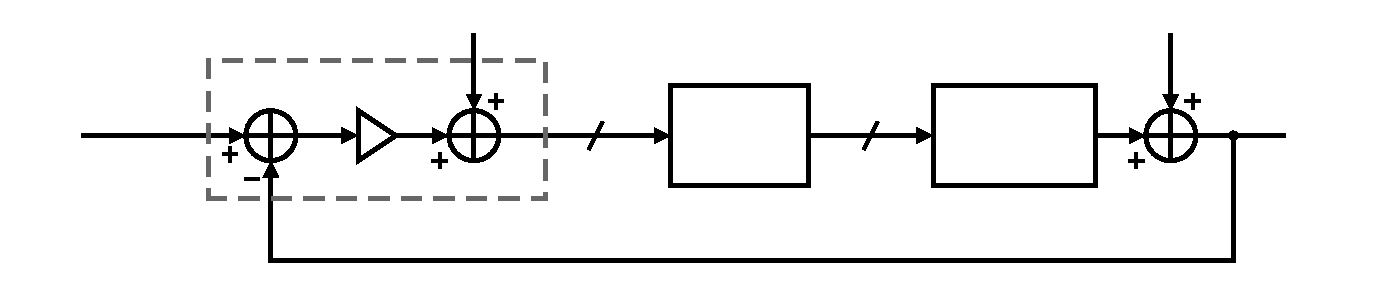
\includegraphics[scale=0.60000]{./figs/bbpll_full_noise.pdf}\\
   % translate x=416 y=448 scale 0.38
   \putbox{0.33600in}{0.70800in}{0.84}{$\Phi_{ref}$(t)}%
   \putbox{2.27400in}{0.73200in}{0.84}{e$_\Phi$(t)}%
   \putbox{1.42200in}{0.78600in}{0.84}{\rotatebox{-360}{$K_{BBPD}$}}%
   \putbox{1.20600in}{0.70800in}{0.84}{$\Phi_e$}%
   \putbox{0.83400in}{0.98400in}{0.84}{BBPD}%
   \putbox{2.77200in}{0.59400in}{0.84}{H$_{LF}$(s)}%
   \putbox{3.39600in}{0.72000in}{0.84}{u(t)}%
   \putbox{3.85800in}{0.60600in}{0.84}{$\frac{2\pi K_{DCO}}{s}$}%
   \putbox{4.82400in}{0.69600in}{0.84}{$\Phi_{out}$(t)}%
   \putbox{3.73200in}{0.87000in}{0.84}{DCO}%
   \putbox{1.93200in}{1.00800in}{0.84}{q$_{n_{BBPD}}$(t)}%
   \putbox{4.72200in}{1.00800in}{0.84}{$\Phi_{n_{DCO}}$(t)}%
   } % close 'parbox'
   } % close 'scalebox'
   \vspace{-\baselineskip} % this is not necessary, but looks better
\fontfamily{\rmdefault}\selectfont

	\caption{BBPD-PLL full noise model.}
	\label{fig:bbpll_full_noise}
\end{figure}

In the divider-based PLL theory (section \ref{sec:pll_output_noise}), the derived PLL detector phase noise component (equation \ref{eq:out_psd_bbpd_pll}) contains a term proportional to $N^2$, that is the detector noise will grow with the square of the PLL divider ratio. It is, however, possible to remove this $N^2$ dependency by usage of oscillator sub-sampling within the PLL \cite{Gao2015}. This is achieved by directly sampling the PLL output at a rate equivalent to the reference frequency. This is equivalent to removing the divider from the PLL loop and directly connecting the PLL output to the phase detector, which has been employed in this work (see figure \ref{fig:pll_arch}). The removal of the divider also removes any PLL noise contributions resulting from divider jitter. 

 In a dividerless PLL, it must be guaranteed that the PLL frequency at the start of sub-sampling operation be within $f_{ref}/2$ of the target frequency (the PLL will lock to the nearest multiple of the reference frequency). In this work, this is achieved through sequencing at startup through two phase detectors. A synchronous counter phase detector (which emulates both a divider and phase detector) initially locks the PLL within $f_{ref}/2$ of the target frequency, after which the PLL is operated in sub-sampling bang-bang phase detector.

  In accordance to the change to a dividerless operation, the PLL closed loop transfer function has been rederived in equation \ref{eq:cont_pll_tf2}. Furthermore, new expressions for PLL output phase noise with a BBPD is given in equation \ref{eq:out_psd_bbpd_pll2}, and PLL output oscillator noise with a ring oscillator is given in equation \ref{eq:out_psd_dco_pll2}, for the noise model in figure \ref{fig:bbpll_full_noise}. Noise due to the loop filter here is ignored, as it will be possible to adjust the loop filter datapath resolution to make digital quantizaiton noise effects negligible.
		\begin{align} \label{eq:cont_pll_tf2}
			\mathrm{T}(s) = \frac{\Phi_{out}(s)}{\Phi_{ref}(s)} = \frac{2\pi K_{BBPD}K_{DCO}\sum_{j=0}^Z b_js^j}{\sum_{k=0}^P a_ks^{k+1} + 2\pi K_{BBPD}K_{DCO}\sum_{j=0}^Z b_js^j} = \frac{\mathrm{L}(s)}{1 + \mathrm{L}(s)}
		\end{align}
		\begin{align}\label{eq:out_psd_bbpd_pll2}
			S_{\Phi n_{BBPD,out}}(f) &= S_{n_{BBPD}}(f)\left|\frac{\Phi_{out}(f)}{q_{n_{BBPD}}(f)}\right|^2 = \frac{\left(\frac{\pi}{2}-1\right)}{f_{ref}}\left|\sigma_{\Phi_e}\mathrm{T}(f)\right|^2
		\end{align}
		\begin{align}\label{eq:out_psd_dco_pll2}
			S_{\Phi n_{DCO,out}}(f) &= \mathcal{L}_{min}(f)\left|\frac{\Phi_{out}(f)}{q_{n_{DCO}}(f)}\right|^2 = \frac{7.33k_BT}{P}\left(\frac{f_0}{f}\right)^2|1-\textnormal{T}(f)|^2 
		\end{align}


% ################################################################################################
% ################################################################################################
	\subsection{Bang-Bang Phase Detector}
		A bang-bang phase detector, as introduced in section \ref{bbpd_theory}, can be implemented physically with a D flip-flop \cite{Razavi2020} and logic to map the logical state to a signed $\pm$1 value that may be passed into a digital loop filter. This is shown in figure \ref{fig:bbpd_dff}. 

		\begin{figure}[htb!]
			\center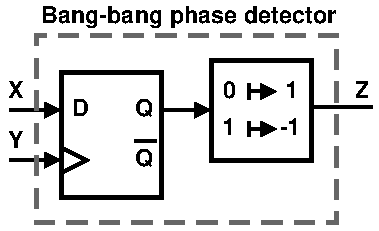
\includegraphics[width=0.4\textwidth, angle=0]{./figs/design/bbpd_}
			\caption{Bang-bang phase detector with D flip-flop.}
			\label{fig:bbpd_dff}
		\end{figure}
		The realization of a BBPD using a digital flip flop introduces additional noise to the system in the form of jitter. Jitter arises as an artifact of circuit and supply noise. For small time differentials between the BBPD inputs X and Y, the output can be stochatically corrupted due to the presence of noise. Furthermore, physical D flip flop implementations exhibit set-up and hold time requirements for data to be stable (to allow internal nodes to settle), so deterministic corruption of phase detection can be imparted if the inputs violate physical timing requirements. These sources of corruption cause BB-PD transfer characteristics in terms of output expectation, $\mathbb{E}[Z]$, with respect to input timing difference $\Delta t_{XY}$ to deviate from an ideal step response, demonstrated in figure \ref{fig:bbpd_jit_pdf}. Analytically, the corruption of the transfer characteristic can be viewed as being caused by an additive phase noise component before the signum operation in the BBPD, as shown in figure \ref{fig:bbpd_noise_nonlinear}. The expectation $\mathbb{E}[Z(\Delta t_{XY})]$ acts as a cumulative distribution function (CDF) for this phase noise component. Thus, differentiation of $\mathbb{E}[Z(\Delta t_{XY})]$ results in a probability distribution function (PDF) P(T=$\Delta t_{xy}$) of this phase noise signal. Statistical analysis of variance of the PDF provides an RMS value for timing jitter of this additive noise source, $\sqrt{\mathrm{Var}[T]} = \sigma_{t,j}$. The RMS timing jitter may be converted to RMS phase error of the noise source as $\sigma_{\Phi_j} = 2\pi f_{osc}\sigma_{t_j}$. This analysis approach is applied in this work to evaluate BBPD performance.
 
		\begin{figure}[htb!]
		    \centering
			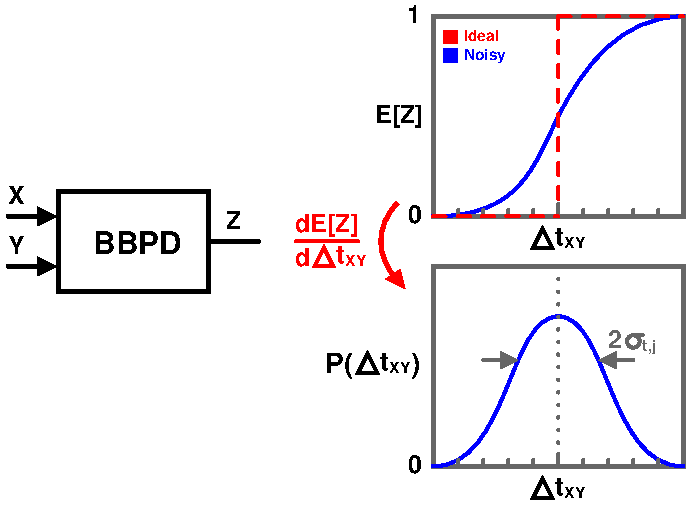
\includegraphics[width=0.6\textwidth, angle=0]{./figs/bbpd_jitter.pdf}
			\caption{BBPD output expectation and jitter PDF versus input time differential.}
			\label{fig:bbpd_jit_pdf}
		\end{figure}

	\begin{figure}[htb!]
	    \centering
	    \begin{subfigure}{0.5\textwidth}
	        \centering
	        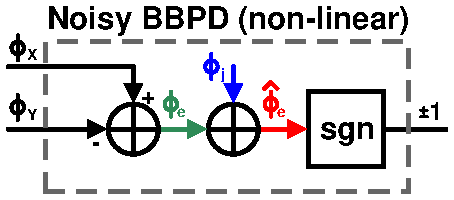
\includegraphics[width=0.8\textwidth, angle=0]{figs/design/bbpd_noise_nonlinear}
	        \caption{ }
	        \label{fig:bbpd_noise_nonlinear}
	    \end{subfigure}%
	    \begin{subfigure}{0.5\textwidth}
	        \centering
	        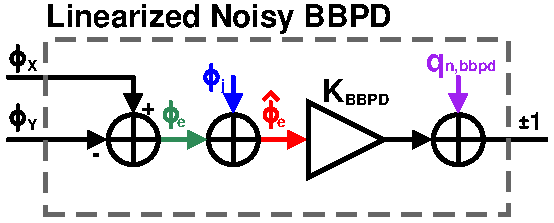
\includegraphics[width=0.9\textwidth, angle=0]{figs/design/bbpd_noise_linear}
	        \caption{ }
	        \label{fig:bbpd_noise_linear}
	    \end{subfigure}
	    % \caption{x.}
	    \caption{\textbf{(a)} Noisy BBPD nonlinear model \textbf{(b)} Noisy BBPD linearized model}
	     \label{fig:bbpd_noisy}
	\end{figure} 

	With a model for BBPD noise due to implementation non-idealities, a modified linearized model for the BBPD will be established here. This model will reconcile the ideal BBPD noise introduced in section \ref{sec:bbpd_noise} with the noise due to the new additive jitter component just described. First, a component representing the non-ideal jitter component, $\Phi_j$, is added into noise model from figure \ref{fig:bbpll_full_noise}. The result is the linearized model of figure \ref{fig:bbpd_noise_linear}. We then define a modified phase error, $\hat{\Phi}_e$, which includes the nominal $\Phi_e$ and the jitter corruption:
	\begin{equation}
	\hat{\Phi}_e = \Phi_e + \Phi_j.
	\end{equation}
	$\hat{\Phi}_e$ has a variance defined as $\sigma_{\hat{\Phi}_e}^2 = \sigma_{\Phi_e}^2 + \sigma_{\Phi_j}^2$, assuming $\Phi_e$ and $\Phi_j$ are uncorrelated. Defining BBPD gain in terms of $\sigma_{\hat{\Phi}_e}$:
	\begin{equation}
		K_{BBPD} = \sqrt{\frac{2}{\pi}}\cdot\frac{1}{\sigma_{\hat{\Phi}_e}} = \sqrt{\frac{2}{\pi}}\cdot\frac{1}{\sqrt{\sigma_{\Phi_e}^2 + \sigma_{\Phi_j}^2}}
	\end{equation}

	 It is then observed that the output Z is valued $\pm$1, thus its power is always $\sigma_Z^2$=1. Furthermore:
	\begin{equation}
	 	\sigma^2_{Z} = 1 = K_{BBPD}^2(\sigma^2_{\phi_e} +\sigma^2_{\phi_j})  + \sigma^2_{q_{n,BBPD}}
	\end{equation}
	 As determined in section \ref{sec:bbpd_noise}, it is inherent that $\sigma^2_{q_{n,BBPD}} = 1 - \frac{2}{\pi}$. If the total output noise
			\begin{equation}
				\sigma^2_{\phi_{n,BBPD}} =  \sigma^2_{q_{n,BBPD}} + K_{BBPD}^2\sigma^2_{\phi_j} =  1 - \frac{2}{\pi}\frac{\sigma^2_{\phi_e}}{\sigma^2_{\phi_j} + \sigma^2_{\phi_e}}
			\end{equation}
	If the BB-PD is connected directly to oscillator output, $\sigma^2_{\phi_e}$ = $\sigma^2_{\phi_n}$, i.e. the PLL output phase noise. The spectral density of the BB-PD phase noise is then:
		\begin{equation}
			S_{\phi_{n,BBPD}} = \frac{\sigma^2_{\phi_{n,BBPD}}}{f_{ref}} =  \frac{1 - \frac{2}{\pi}\frac{\sigma^2_{\phi_n}}{\sigma^2_{\phi_j} + \sigma^2_{\phi_n}}}{f_{ref}}
		\end{equation}

		\begin{align}\label{eq:out_psd_bbpd_pll3}
			S_{\Phi n_{BBPD,out}}(f) &= S_{n_{BBPD}}(f)\left|\frac{\Phi_{out}(f)}{q_{n_{BBPD}}(f)}\right|^2 = \frac{\frac{\pi}{2}(\sigma^2_{\phi_j} + \sigma^2_{\phi_n})-\sigma^2_{\phi_n}}{f_{ref}}\left|\mathrm{T}(f)\right|^2
		\end{align}

	% \begin{itemize}[itemsep=4pt,label=\protect---]
	% 	\item It is observed that PLL phase noise spectrum is approximately Lorentzian (except for peaking and flicker noise components). Given BB-PD noise PSD of $S_{\phi_{n,BBPD}}$, and an oscillator with noise PSD $S_{\phi_{n,osc}}(\Delta f)$, the optimal bandwidth for minimum noise power is:

	% 	\begin{equation}
	% 		BW_{opt} =  \sqrt{\frac{S_{\phi_{n,osc}}(\Delta f)}{S_{\phi_{n,BBPD}}}}\Delta f
	% 	\end{equation}
	% 	\item The total PLL output phase noise with optimal bandwidth is then:

	% 	\begin{equation}
	% 		\sigma^2_{\phi_{n,opt}} =   \pi\sqrt{\phi_{n,osc}(\Delta f)S_{\phi_{n,BBPD}}}\Delta f
	% 	\end{equation}
	% \end{itemize}
	% \vspace{-3em}
	% \begin{figure}[htb!]
	%     \centering
	%     \begin{subfigure}{0.33\textwidth}
	%         \centering
	%         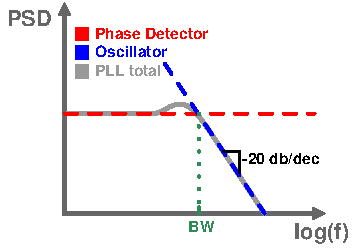
\includegraphics[width=1\textwidth, angle=0]{./figs/pll_spectrum_lorentzian.pdf}
	%     \end{subfigure}%
	%     \begin{subfigure}{0.33\textwidth}
	%         \centering
	%         \center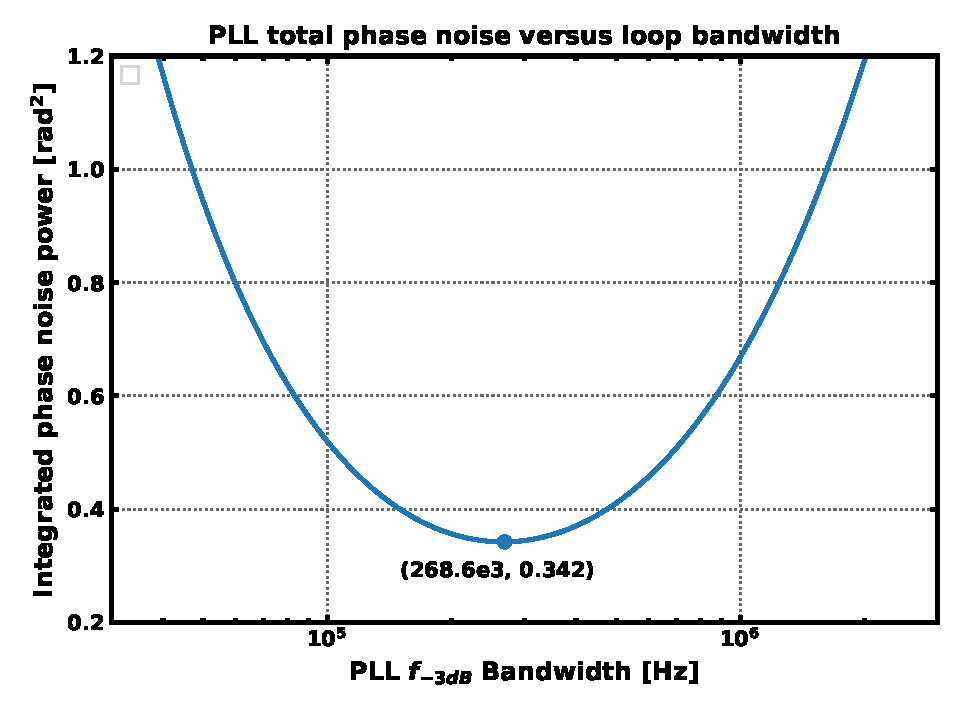
\includegraphics[width=1.0\textwidth, angle=0]{./figs/bandwidth_vs_pn.pdf}
	%     \end{subfigure}
	%     % \caption{Approximate model for ring oscillator inverter delay cell.}
	% \end{figure}




	% \begin{itemize}[itemsep=4pt,label=\protect---]
	% 	\item Using the findings for BB-PD noise PSD, assumption of Lorentzian spectrum, and constraint that BW = $\alpha f_{ref}$ (recommended $\alpha$$<$0.1 [2], rule of thumb since ancient PLL days). Given oscillator center frequency $f_c$, BB-PD jitter is constrained:

	% 	\begin{equation}
	% 		\sigma_{t_j} \leq \frac{\sigma_{\Phi_n}}{2\pi f_c}\sqrt{\frac{2}{\pi}\left(\frac{1}{\pi\alpha} - \frac{\pi}{2} + 1\right)} = \frac{\sigma_{\Phi_n}}{2\pi f_c}\beta(\alpha)
	% 	\end{equation}
	% 	\item $\beta(\alpha=0.1)$ = 1.28, $\beta(\alpha=0.05)$ = 1.92.
	% 	\item Using my PLL specifications ($f_c$ = 2.448 GHz, CNR = -$\sigma_{\Phi_n}$ = 17 dB, $\alpha=0.1$), {\color{red}\textbf{$\sigma_{t,j}\leq 11.8 $ ps}}
	% \end{itemize}



	% \begin{itemize}[itemsep=4pt,label=\protect---]
	% 	\item With an unconstrained relationship for BW and $f_{ref}$, and the optimal bandwidth finding, it is determined that the optimal value of $\sigma_{t,j}$ for minimum phase noise is:

	% 	\begin{equation}
	% 		\sigma_{t_j,opt} = \frac{\sigma_{\Phi_n}}{2\pi f_c}\sqrt{\frac{2}{\pi}\left[\frac{\sigma^4_{\Phi_n} f_{ref}}{\pi^2 S_{\phi_{n,osc}}(\Delta f) \Delta f^2} - \left(\frac{\pi}{2} - 1\right)\sigma^2_{\Phi_n}\right]}
	% 	\end{equation}

	% \end{itemize}

	% \begin{itemize}[itemsep=4pt,label=\protect---]
	% 	\item Setting the two jitter equations of the last side equal, it is found that optimal phase noise power is:

	% 	\begin{equation}
	% 		\sigma^2_{\Phi_n, opt} = \frac{\pi S_{\phi_{n,osc}}(\Delta f) \Delta f^2}{\alpha f_{ref}}
	% 	\end{equation}
	% 	\item The optimal reference frequency ($\sigma_{\Phi_n}=2\pi f_c \sigma_{t_n}$ = CNR):
	% 	\begin{equation}
	% 		f_{ref} = \frac{\pi S_{\phi_{n,osc}}(\Delta f) \Delta f^2}{\alpha \sigma^2_{\Phi_n}}
	% 	\end{equation}
	% 	\item The optimal oscillator phase noise at offset $\Delta f$:
	% 	\begin{equation}
	% 		S_{\phi_{n,osc}}(\Delta f) = \frac{\alpha f_{ref}\sigma^2_{\Phi_n}}{\pi \Delta f^2} 
	% 	\end{equation}
	% 	\item For CNR = 17 dB, $S_{\phi_{n,osc}}(\Delta f = 1 MHz)$ = -80 dBc/Hz, $\alpha$ = 0.1, {\color{red}the optimal $f_{ref}$ = 15.7 MHz.}
	% 	\item For CNR = 20 dB, $S_{\phi_{n,osc}}(\Delta f = 1 MHz)$ = -80 dBc/Hz, $\alpha$ = 0.1, {\color{red}the optimal $f_{ref}$ = 31.4 MHz.}
	% \end{itemize}


		\FloatBarrier






		\subsubsection{Circuit}
		The physcial implementation of the bang-bang phase detector has been selected to utilize a true single phase clock (TSPC) D-flip flop \cite{Yuan1989}. The positive-edge triggered variant of this circuit has been implemented as shown in figure \ref{fig:tspc_dff}. Selection of this topology was based on the desire for the usage of a single ended clock as a reference signal.

			\begin{figure}[htb!]
			        \centering
			        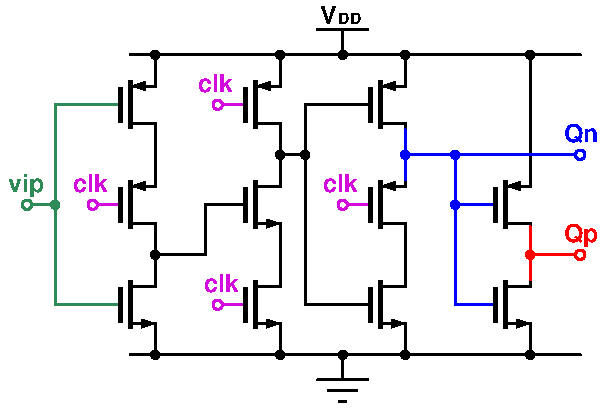
\includegraphics[width=0.6\textwidth, angle=0]{./figs/design/tspc_}
			    \caption{True single-phase clock (TSPC) D flip-flop, positive edge triggered.}
			    \label{fig:tspc_dff}
			\end{figure}

		This TSPC design was validated in simulation with RVT devices with all devices set with (W/L) = \{100n/20n, 200n/20n\}, and with supply voltages of 0.5 and 0.8 volts. Results for the RMS jitter and power consumption are in table \ref{tab:dff}. For implementation (W/L) = 200n/20n was selected for all devices, as the requirement of 10 $\mu$W is met with layout parasitics, whilst having low jitter.


		% \end{itemize}
		% % \vspace{-3em}
		% \begin{figure}[htb!]
		%     \centering
		%     \begin{subfigure}{0.5\textwidth}
		%         \centering
		%         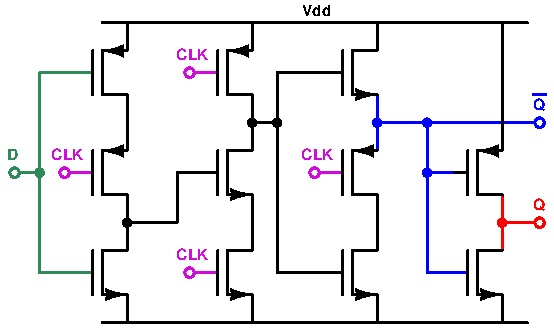
\includegraphics[width=0.8\textwidth, angle=0]{./figs/tspc_dff.pdf}
		%         \caption{TSPC DFF}
		%     \end{subfigure}%
		%     \begin{subfigure}{0.5\textwidth}
		%         \centering
		%         \center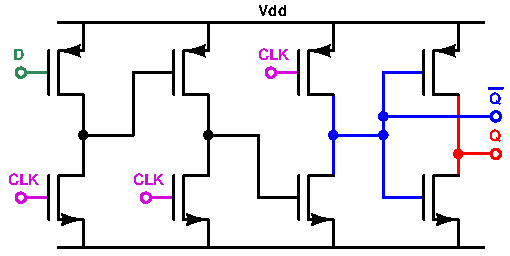
\includegraphics[width=0.8\textwidth, angle=0]{./figs/etspc_dff.pdf}
		%         \caption{e-TSPC DFF}
		%     \end{subfigure}
		%     % \caption{Approximate model for ring oscillator inverter delay cell.}
		% \end{figure}


	% \begin{itemize}[itemsep=4pt,label=\protect---]
	% 	\item Utilized TSPC DFF, with inverter buffers (FETs sized 200n/20n) for clock and data buffers.
	% 	\item Sweep delay between inputs, calculating the expect value of the output for 100 bits. Transient noise simulated (up to 100 GHz), and the inital state of the FF is set to be high 50x and low 50x to include hysteresis effects. 
	% 	\item V$_{DD} \in$ \{0.5, 0.8\} V and (W/L) $\in$ \{100n/20n, 200n/20n\} tested. 100 aF added to every node.
	% 	\item \textbf{Resulting CDFs of the input time delta versus output expectation are below.}
	% \end{itemize}
	% \vspace{-2em}
	% \begin{figure}[htb!]
	%     \centering
	% 	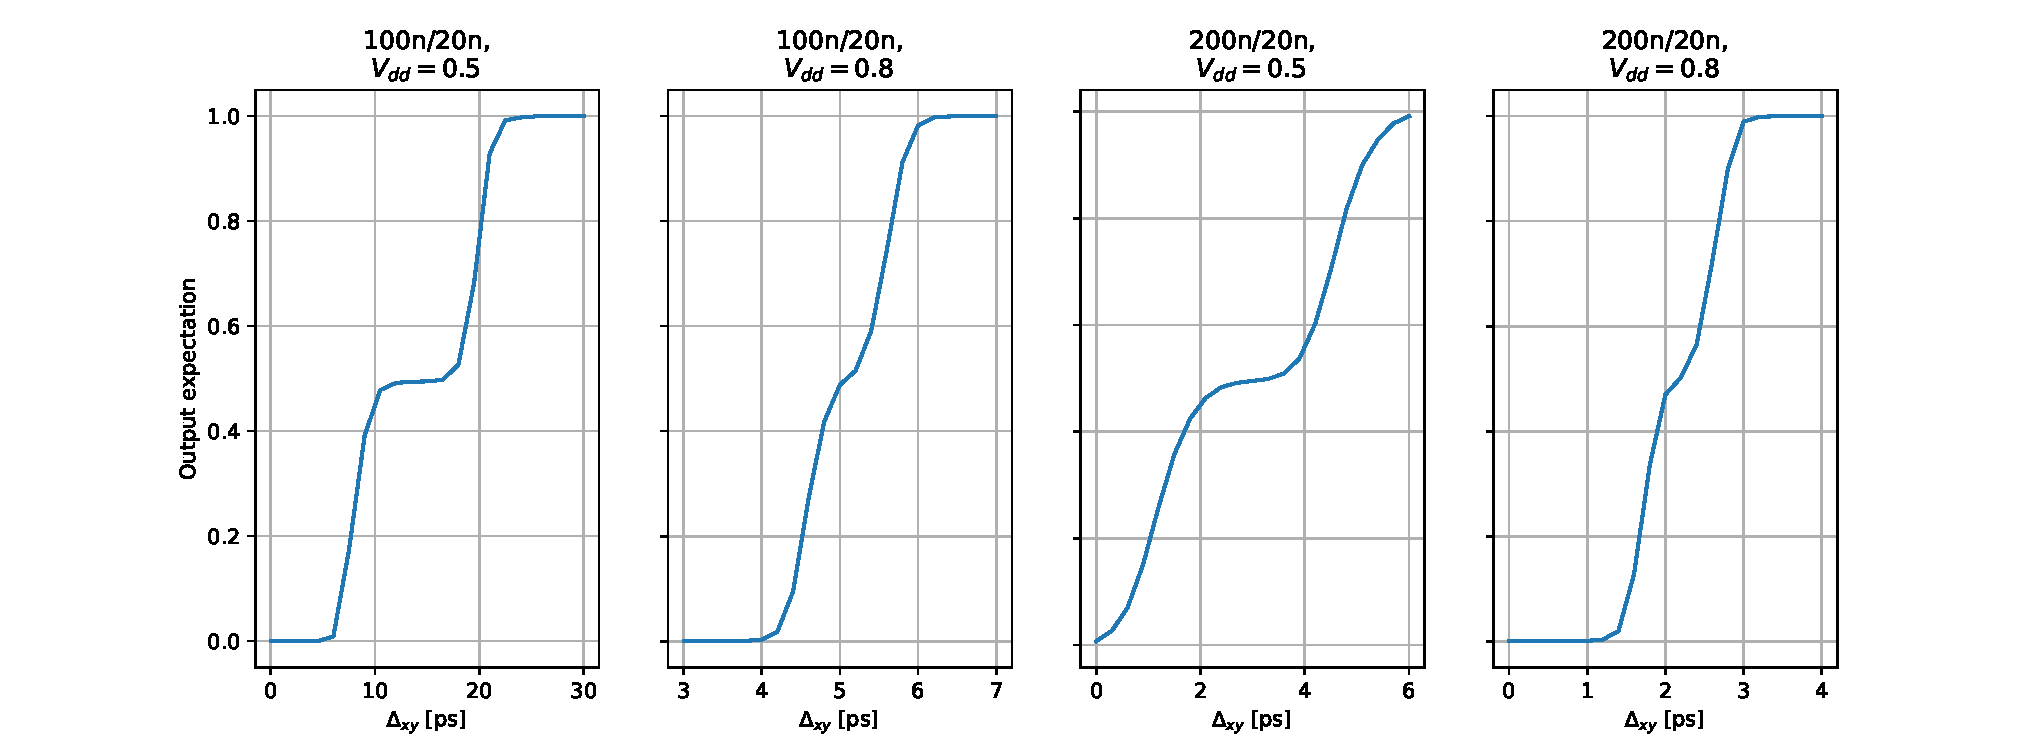
\includegraphics[width=1\textwidth, angle=0]{./figs/cdfs.pdf}
	% \end{figure}

	% \begin{itemize}[itemsep=4pt,label=\protect---]
	% 	\item Jitter PDFs are bimodal from hysteresis of DFF. 
	% 	\item Increasing (W/L) or $V_{DD}$ both impact jitter favorably.
	% 	\item \textbf{The jitter PDF (computed from the CDFs) of the input time delta versus output expectation are below. (Delays are removed)}
	% \end{itemize}
	% \vspace{-2em}
	% \begin{figure}[htb!]
	%     \centering
	% 	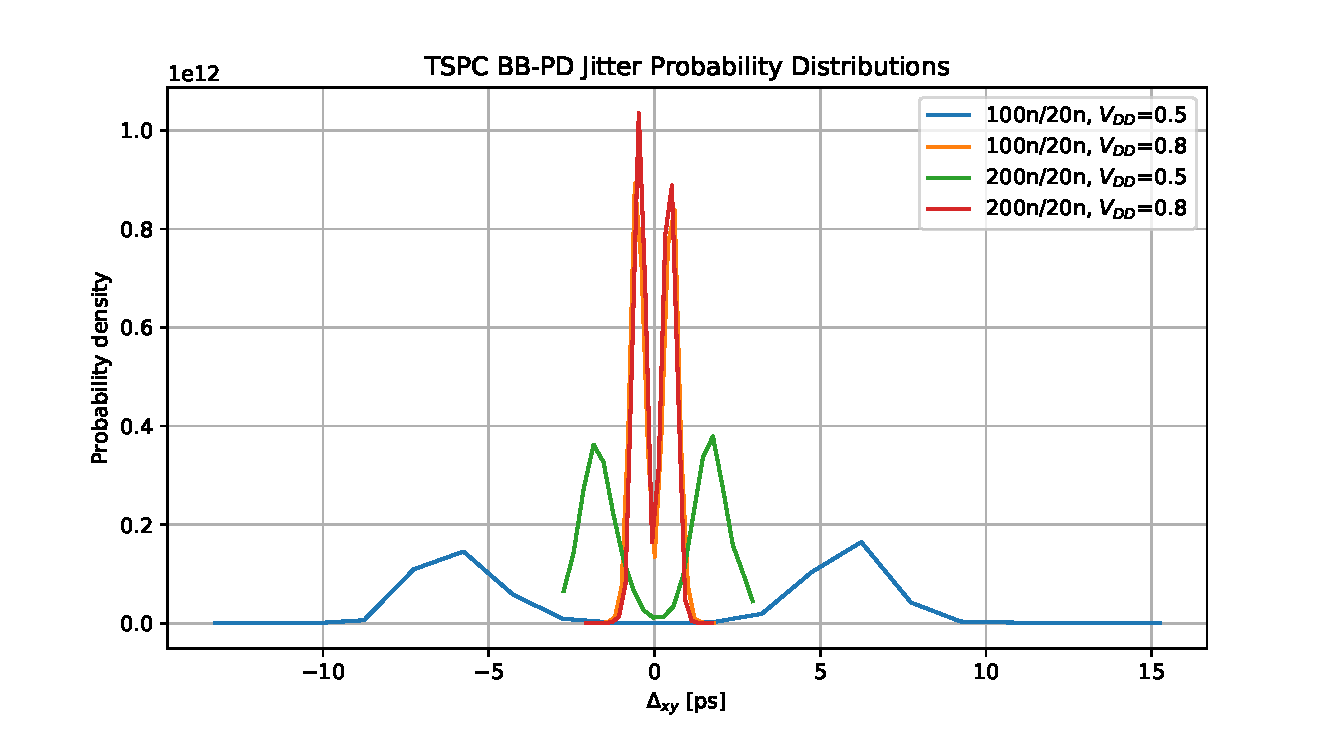
\includegraphics[width=0.7\textwidth, angle=0]{./figs/jitter_pdfs.pdf}
	% 	\caption{Jitter PDF from simulated TSPC DFFs.}
	% 	\label{fig:tspc_dff_sim}
	% \end{figure}


		\begin{table}[h!]
			\centering
			\def\arraystretch{1.5}		
			\setlength\arrayrulewidth{0.75pt}
			\setlength{\tabcolsep}{1em} % for the horizontal padding
			\begin{tabular}{|c|c|c|c|}
				\hline 
				\rule[-1ex]{0pt}{2.5ex} \cellcolor{gray!40}\textbf{(W/L)} & \cellcolor{gray!40}\textbf{Supply [V]} & \cellcolor{gray!40}\textbf{RMS jitter [ps]}& \cellcolor{gray!40}\textbf{Power [$\mu$W]}\\ 
				\hline 
				\rule[-1ex]{0pt}{2.5ex} 100n/20n  & 0.5 & 6.01 & 1.64\\ 
				\hline 
				\rule[-1ex]{0pt}{2.5ex} 100n/20n  & 0.8 & 0.832  & 3.942\\ 
				\hline 
				\rule[-1ex]{0pt}{2.5ex} 200n/20n  & 0.5 & 1.776 & 2.215 \\ 
				\hline 
				\rule[-1ex]{0pt}{2.5ex} 200n/20n  & 0.8 & 0.496  & 4.591 \\ 
				\hline 
			\end{tabular} 
			\caption{Schematic simulation of TSPC DFF.}
			\label{tab:dff}
		\end{table}   
		\FloatBarrier{\color{white}.}







		% \FloatBarrier
		% \subsubsection{Layout}
		% 	\hl{Area?}
		% 	\begin{figure}[htb!]
		% 	        \centering
		% 	        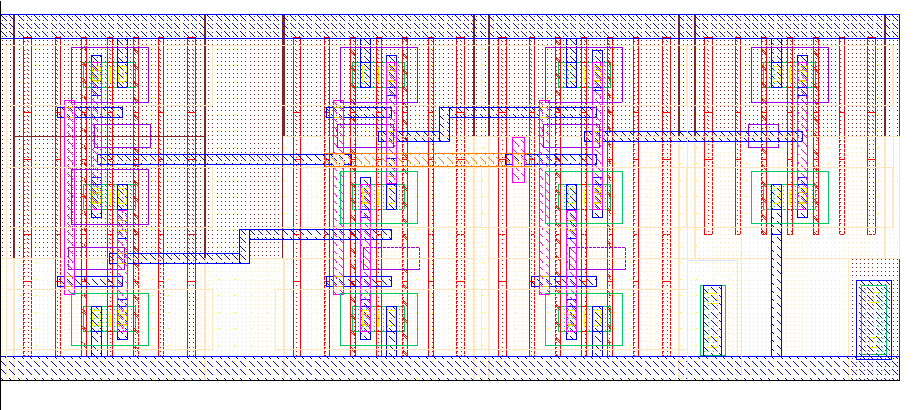
\includegraphics[width=\textwidth, angle=0]{./figs/layout/layout_bbpd}
		% 	    \caption{Single ended bang-bang phase detector.}
		% 	\end{figure}

% ################################################################################################
% ################################################################################################


\FloatBarrier\pagebreak
\subsection{Voltage Controlled Ring oscillator}
	Oscillator circuits implemented in CMOS technology either fall under the catagory of resonant LC circuits, or RC based ring and relaxation oscillators. LC circuits provide favorable phase noise performance, as seen in figure \ref{fig:lc_ro_fom}, which demonstrates phase noise improvements on the order of 20 dB for LC designs over RC designs that have been published. This is due to the inherent nature of an LC circuit, as the higher the quality factor it has, the narrower the resonance line width and consequent phase noise is. In the ultra-low power domain of this work, however, ring oscillators pose several advantages over LC designs. These include substantially smaller integration area due to no need for integrated inductors, simpler design, convenient rail-to-rail signal levels, and lower achievable minimum power at a given frequency. Also significant, is the ability to instantly start up a ring oscillator, which can be achieved with known phase if using appropriate reset circuitry. Coupled with the BBPD, which is a phase only detector (which is not able to detect frequency), the ability to start the oscillator with a known zero-phase, in tandem with being able to set the digital loop filter to a zeroed state, enables faster and more consistant locking compared to randomized initial phase. With the intent of this design to allow for fast duty cycled operation, the need for fast start up is imperative, thus for this reason the ring oscillator topology has been selected for this work. 

	It has been decided in this work to exploit the ability of the FD-SOI backgate terminal to alter threshold voltage in order to implement a backgate voltage controlled ring oscillator as the main PLL VCO. As will be shown in the following sections, backgate tuning results in transconductor modulation within the ring oscillator, which therefore modulates the RC time constant of the delay stages, and consequently the frequency of oscillation. A novel delay cell topology which exploits FD-SOI backgates to implement both differential operation and frequency is subsequently introduced. The described design enables usage of capacitive DACs to set oscillator control voltages, leading to minimal extra power consumption needed to convert the voltage controlled ring oscillator into a DCO. 




			\FloatBarrier
	\subsubsection{22FDX considerations}
		To analyze the body effect through FD-SOI backgates in 22FDX, SPICE simulations to extract the body effect coefficient $\gamma$ and theshold voltage $V_{TH}$ for different channel lengths and bias conditions have been performed. Parameters for threshold voltage, and transconductances $g_m$ and $g_{mb}$ have been extracted using DC operating point simulations. Noting the relation from \ref{eq:gm_gmb_relation}, where $g_{mb} = \gamma g_{m}$, $\gamma$ can be deduced from operating point $g_m$ and $g_{mb}$ values. Figures \ref{fig:vth_vs_vbs} and \ref{fig:vth_slope_vs_vbs} show the extracted threshold voltage versus backgate bias and the slope of that relationship. Figures \ref{fig:vth_vs_len} and \ref{fig:gamma_vs_len} show the extracted theshold voltage and body effect coefficient versus channel length. Table \ref{tab:nfet_vth_gamma} provides extracted N-channel device parameters, and table \ref{tab:pfet_vth_gamma} provides extracted P-channel devices parameters.

		It is observed that the threshold voltage slopes of figure \ref{fig:vth_groupa} are not perfectly linear, but for the simplified analytical purposes of this work, they can be approximated as linear. The P-channel devices in 22FDX show a high degree of linearity, whereas the N-channel devices show variation in slope as in figure \ref{fig:vth_slope_vs_vbs}. It is also observed that the threshold voltage and body effect coefficient vary as channel lengths approach zero, but flatten out for longer device length. A final note is there is substantial variation of $\gamma$ and $V_{TH}$ between device types, so prudent care must be taken in the oscillator for selection of devices and their sizing.

		\begin{equation}
		V_{th} = V_{th0} - \gamma V_{BS}
		\end{equation}

		\begin{figure}[htb!]
		    \centering
		    \begin{subfigure}{0.5\textwidth}
		        \centering
		        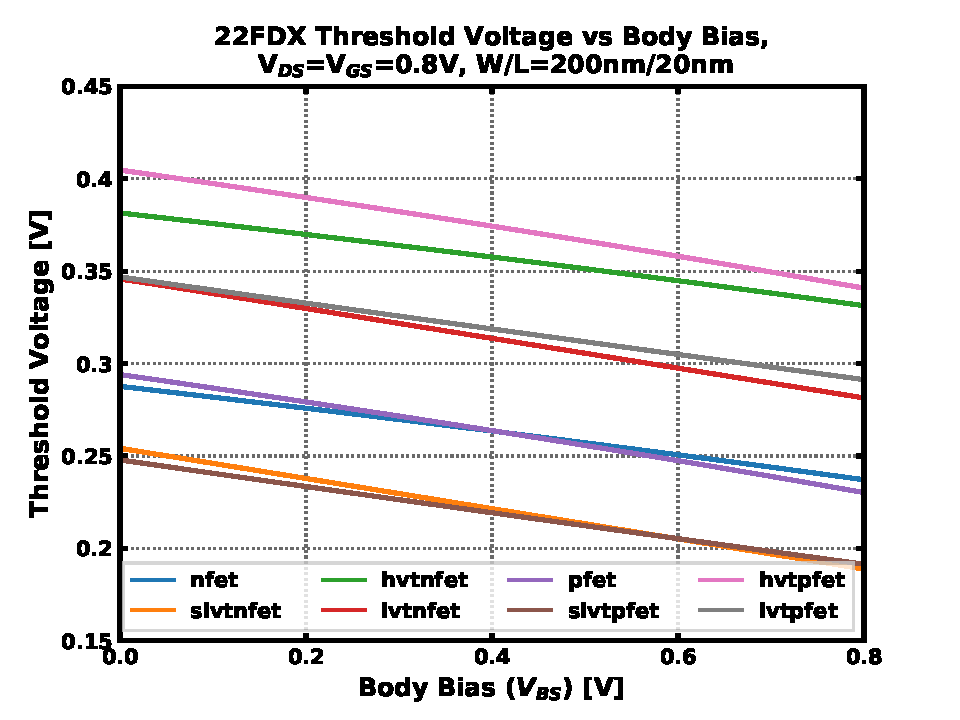
\includegraphics[width=1\textwidth, angle=0]{./figs/design/vth_vbs}
		        \caption{ }
		        \label{fig:vth_vs_vbs}
		    \end{subfigure}%
		    \begin{subfigure}{0.5\textwidth}
		        \centering
		        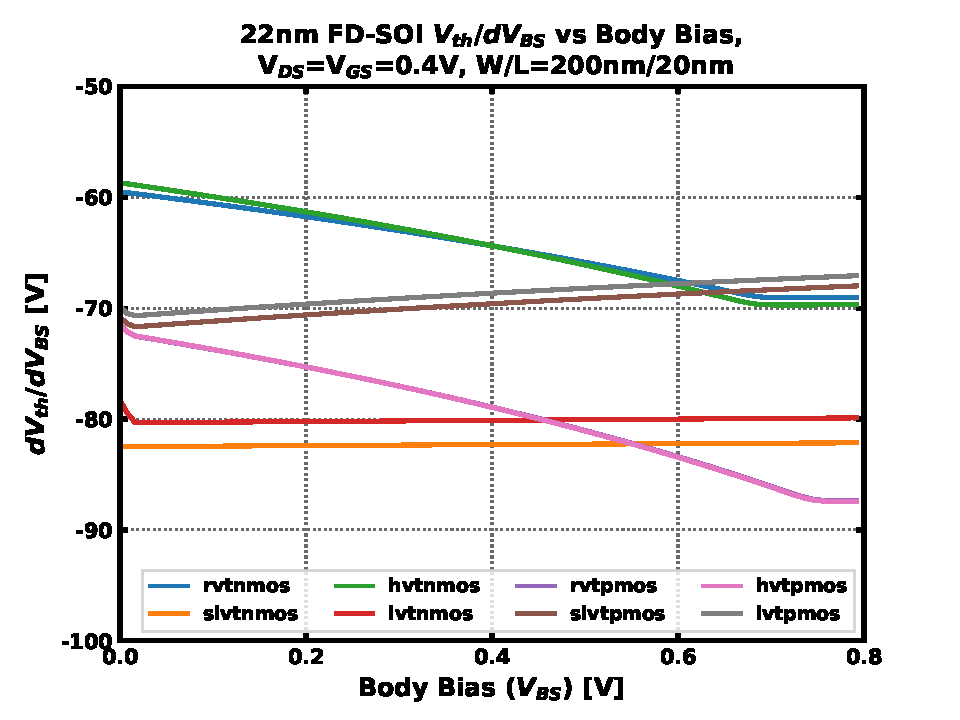
\includegraphics[width=1\textwidth, angle=0]{./figs/design/vth_slope_vbs}
		        \caption{ }
		        \label{fig:vth_slope_vs_vbs}
		    \end{subfigure}
		    % \caption{x.}
		    \caption{\textbf{(a)} 22 FDX threshold voltage versus body bias, \textbf{(b)} Rate of change of threshold voltage versus body bias.}
		    \label{fig:vth_groupa}
		\end{figure} 


		\begin{figure}[htb!]
		    \centering
		    \begin{subfigure}{0.5\textwidth}
		        \centering
		        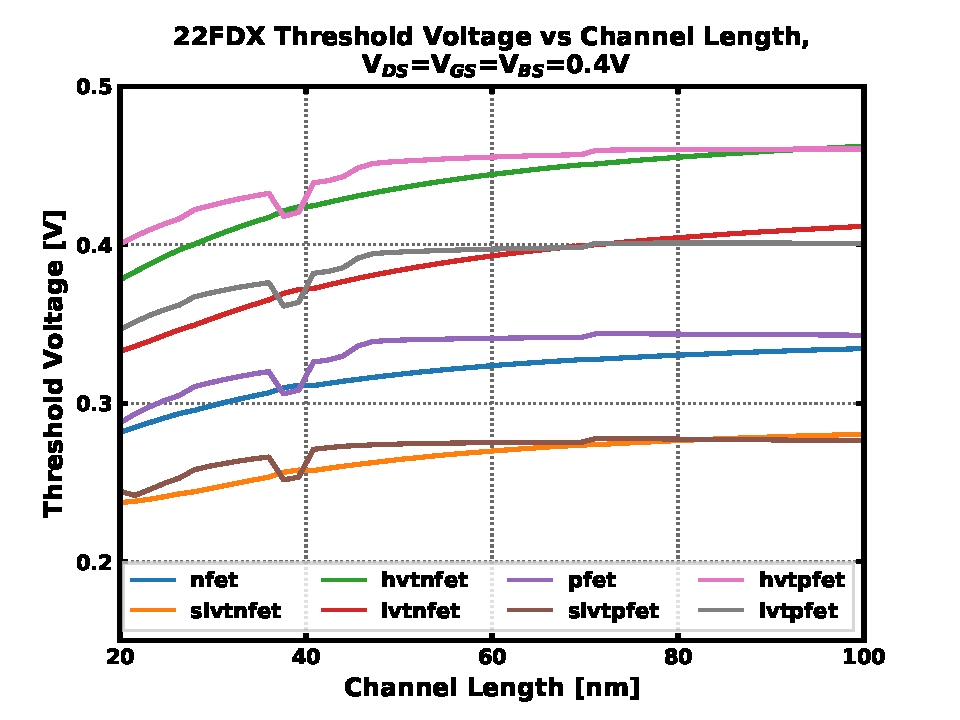
\includegraphics[width=1\textwidth, angle=0]{./figs/design/vth}
		        \caption{ }
		        \label{fig:vth_vs_len}
		    \end{subfigure}%
		    \begin{subfigure}{0.5\textwidth}
		        \centering
		        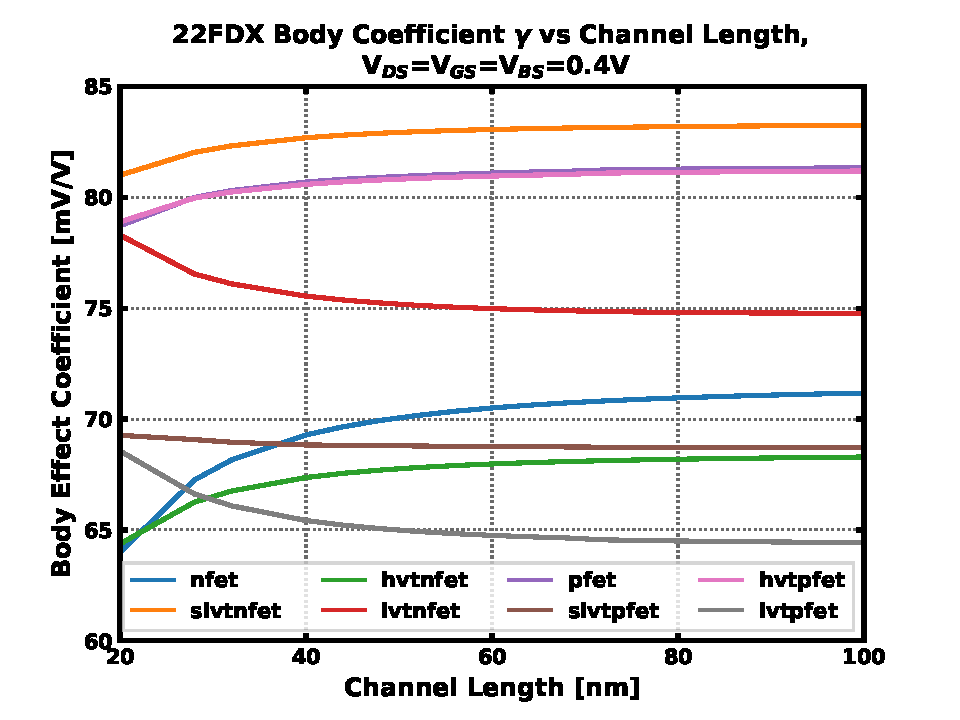
\includegraphics[width=1\textwidth, angle=0]{./figs/design/gamma}
		        \caption{ }
		        \label{fig:gamma_vs_len}
		    \end{subfigure}
		    % \caption{x.}
		    \label{fig:vth_groupb}
		    \caption{\textbf{(a)} 22 FDX Extracted threshold voltage versus channel length, \textbf{(b)} Extracted body effect coefficient.}
		\end{figure} 


			\begin{table}[htb!]
				\centering
				\def\arraystretch{1.5}		
				\setlength\arrayrulewidth{1pt}
				\setlength{\tabcolsep}{1em} % for the horizontal padding
				\fontfamily{\sfdefault}\selectfont 
				\begin{tabular}{|l|l|l|l|l|}	
					\hline 
					\rule[-1ex]{0pt}{2.5ex} \cellcolor{gray!40}\textbf{Device} & \cellcolor{gray!40}\textbf{L [nm]} & \cellcolor{gray!40}\textbf{W [nm]} & \cellcolor{gray!40}\textbf{$V_{th}$ [mV]} & \cellcolor{gray!40}\textbf{$\gamma$ [mV/V]}\\ 
					\hline 
					\rule[-1ex]{0pt}{2.5ex} \textbf{nfet} & 20 & 100 & 306.3 & 59.14 \\ 
					\hline 
					\rule[-1ex]{0pt}{2.5ex} \textbf{nfet} & 100 & 500 & 376.4 & 65.4 \\ 
					\hline 
					\rule[-1ex]{0pt}{2.5ex} \textbf{slvtnfet} & 20n & 100 & 270.3 & 81.38 \\ 
					\hline 
					\rule[-1ex]{0pt}{2.5ex} \textbf{slvtnfet} & 100 & 500 & 326.7 & 83.23 \\ 
					\hline 
					\rule[-1ex]{0pt}{2.5ex} \textbf{hvtnfet} & 20n & 100 & 402.4 & 58.85 \\ 
					\hline 
					\rule[-1ex]{0pt}{2.5ex} \textbf{hvtnfet} & 100 & 500 & 513.5 & 61.96 \\ 
					\hline 
					\rule[-1ex]{0pt}{2.5ex} \textbf{lvtnfet} & 20 & 100 & 364.9 & 77.72 \\ 
					\hline 
					\rule[-1ex]{0pt}{2.5ex} \textbf{lvtnfet} & 100 & 500 & 466.3 & 74.85 \\ 
					\hline 
				\end{tabular} 
				\caption{22FDX core NFET threshold voltage and body effect coefficient extraction.}
				\label{tab:nfet_vth_gamma}
			\end{table} 

			\begin{table}[htb!]
				\centering
				\def\arraystretch{1.5}		
				\setlength\arrayrulewidth{1pt}
				\setlength{\tabcolsep}{1em} % for the horizontal padding
				\fontfamily{\sfdefault}\selectfont 
				\begin{tabular}{|l|l|l|l|l|}	
					\hline 
					\rule[-1ex]{0pt}{2.5ex} \cellcolor{gray!40}\textbf{Device} & \cellcolor{gray!40}\textbf{L [nm]} & \cellcolor{gray!40}\textbf{W [nm]} & \cellcolor{gray!40}\textbf{$V_{th}$ [mV]} & \cellcolor{gray!40}\textbf{$\gamma$ [mV/V]}\\ 
					\hline 
					\rule[-1ex]{0pt}{2.5ex} \textbf{pfet} & 20 & 100 & 317.7 & 71.51 \\ 
					\hline 
					\rule[-1ex]{0pt}{2.5ex} \textbf{pfet} & 100 & 500 & 366.8 & 74.32 \\ 
					\hline 
					\rule[-1ex]{0pt}{2.5ex} \textbf{slvtpfet} & 20n & 100 & 272.6 & 71.09 \\ 
					\hline 
					\rule[-1ex]{0pt}{2.5ex} \textbf{slvtpfet} & 100 & 500 & 294.4 & 70.79 \\ 
					\hline 
					\rule[-1ex]{0pt}{2.5ex} \textbf{hvtpfet} & 20n & 100 & 430.7 & 71.28 \\ 
					\hline 
					\rule[-1ex]{0pt}{2.5ex} \textbf{hvtpfet} & 100 & 500 & 488.4 & 74.23 \\ 
					\hline 
					\rule[-1ex]{0pt}{2.5ex} \textbf{lvtpfet} & 20 & 100 & 374.2 & 69.93 \\ 
					\hline 
					\rule[-1ex]{0pt}{2.5ex} \textbf{lvtpfet} & 100 & 500 & 422.8 & 66.43 \\ 
					\hline 
				\end{tabular} 
				\caption{22FDX core PFET threshold voltage and body effect coefficient extraction.}
				\label{tab:pfet_vth_gamma}
			\end{table} 	
\FloatBarrier

\subsubsection{Channel length consideration}
	Scaling of device channel length has a great impact on phase noise for ring oscillators, according to \cite{Liu2020} takes form of equation \ref{eq:liu_pn_scaling}. $V_{DD}$ is the supply voltage, $V_t$ is the threshold voltage, $P_{DC}$ is the oscillator power consumption, $\gamma p$ and $\gamma n$ are the respective PMOS and NMOS noise factors, $f_0$ is the oscillator frequency, and $f$ is the offset from the carrier for the phase noise. It is expected that excess noise factor of the transistor will increase with decreasing channel length \cite{Antonopoulos2013}, thus unavoidably phase noise will also increase with decreasing length following equation \ref{eq:liu_pn_scaling}. To analyze the effect of channel length on ring oscillator performance in 22FDX technology, a 5-stage single ended ring oscillator was simulated for channel lengths between 20-500nm, with a fixed (W/L)=5 and no external loading. The resulting phase noise FOM$_{pn}$ data is shown in figure \ref{fig:rosc_fom}, oscillator frequency in figure \ref{fig:rosc_freq}, oscillator power in figure \ref{fig:rosc_power}, and phase noise at offset 1 MHz from the carrier in figure \ref{fig:rosc_pn_1m}. The phase noise FOM is that defined in equation \ref{eq:fom_pn}. It is seen that FOM degrades as expected near minimum channel length, and improves asymptotically as the channel length grows. The asymptote closely correlates to that predicted theoretically for RC based oscillators, in equation \ref{eq:ro_fom_limit}. At 300K, as simulated, this is -165.2 dB. Better (i.e. lower valued) FOM corresponds to better phase noise per unit of oscillator power expenditure. Thus, based on the data of figure \ref{fig:rosc_fom}, the best design strategy to minimize phase noise for a fixed power budget is to use the longest possible channel length. Channel length limits frequency of operation, as seen in figure \ref{fig:rosc_freq}, so there is a trade off between frequency of operation and achievable FOM. 

	\begin{equation} \label{eq:liu_pn_scaling}
		\mathcal {L}(f) =\frac {2kT}{P_{\textrm {DC}}}\left ({\frac {V_{\textrm {DD}}}{V_{\textrm {DD}}-V_{t}} (\gamma _{N}+\gamma _{P}+1)}\right)\left ({\frac {f_{0}}{f}}\right)^{2}
	\end{equation}

		\begin{figure}[htb!]
		    \centering
		    \begin{subfigure}{0.5\textwidth}
		        \centering
		        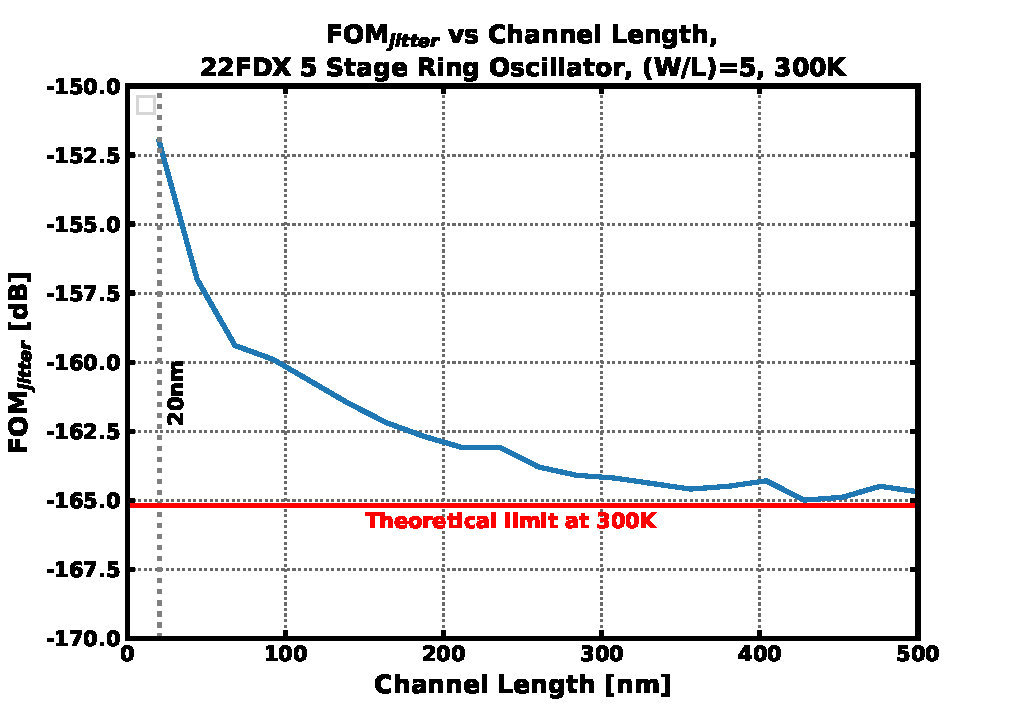
\includegraphics[width=1\textwidth, angle=0]{./figs/design/22fdx_rosc_fom}
		        \caption{ }
		        \label{fig:rosc_fom}
		    \end{subfigure}%
		    \begin{subfigure}{0.5\textwidth}
		        \centering
		        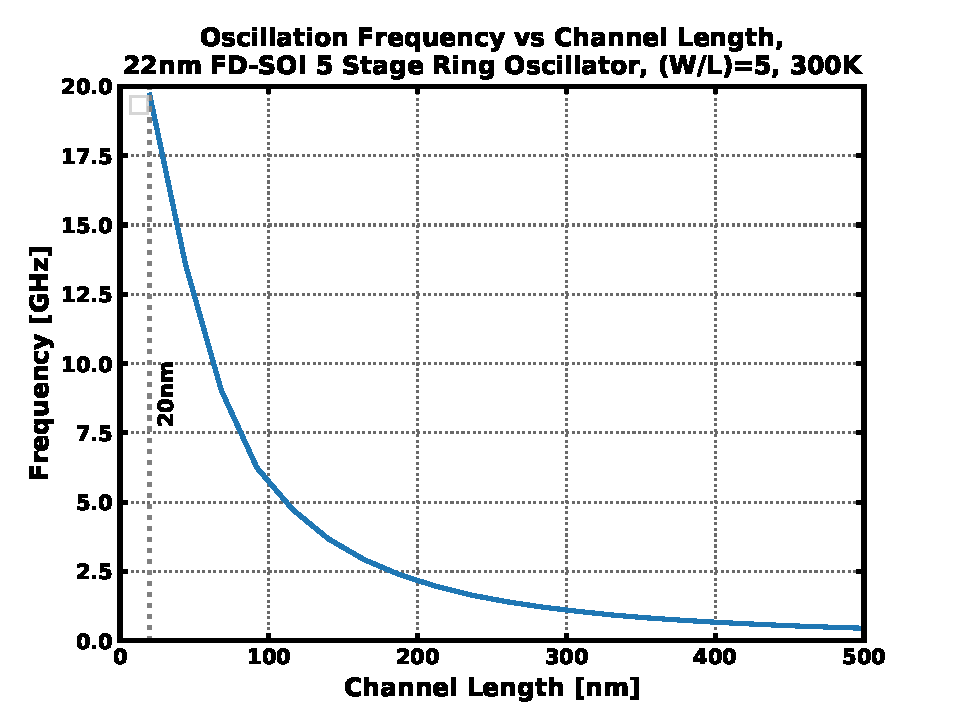
\includegraphics[width=1\textwidth, angle=0]{./figs/design/22fdx_rosc_freq}
		        \caption{ }
		        \label{fig:rosc_freq}
		    \end{subfigure}
		    % \caption{x.}
		    \label{fig:rosc_groupa}
		    \caption{22FDX ring oscillator channel length sweep versus \textbf{(a)} FOM, \textbf{(b)} Oscillation frequency.}
		\end{figure} 	

		\begin{figure}[htb!]
		    \centering
		    \begin{subfigure}{0.5\textwidth}
		        \centering
		        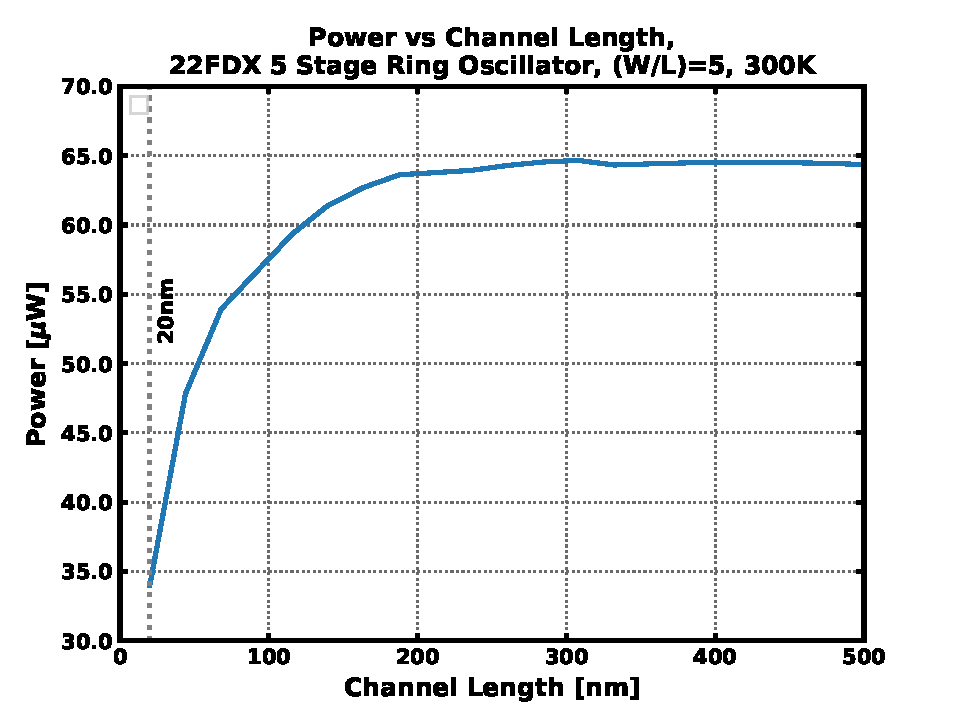
\includegraphics[width=1\textwidth, angle=0]{./figs/design/22fdx_rosc_power}
		        \caption{ }
		        \label{fig:rosc_power}
		    \end{subfigure}%
		    \begin{subfigure}{0.5\textwidth}
		        \centering
		        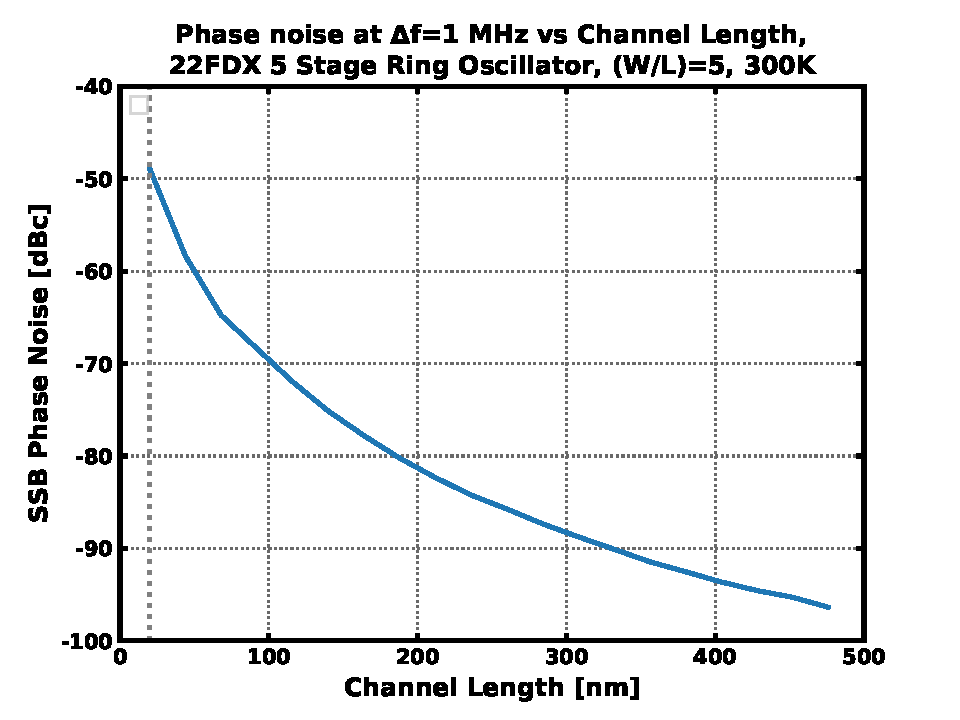
\includegraphics[width=1\textwidth, angle=0]{./figs/design/22fdx_rosc_pn_1mhz}
		        \caption{ }
		        \label{fig:rosc_pn_1m}
		    \end{subfigure}
		    % \caption{x.}
		    \label{fig:rosc_groupb}
		    \caption{22FDX ring oscillator channel length sweep versus \textbf{(a)} Power, \textbf{(b)} Phase noise at 1 MHz carrier offset (SSB).}
		\end{figure} 

	\FloatBarrier


	\subsubsection{Ring oscillator frequency derivation}
		To analyze the effect of backgate tuning on a FD-SOI ring oscillator, a general mathematical model for CMOS ring oscillators will be developed first here. To begin, an approximate model for a CMOS inverter will first be considered. A common model for delay in digital circuits is an RC circuit, where the MOSFET channels are approximated with an averaged conductance value $\langle g_{ch} \rangle$, and the output node is approximated to have a capacitance of C. With such a model, a ring oscillator would be assumed to have waveforms as decaying exponential, with time constant $\tau = \langle g_{ch} \rangle^{-1}C$. In context of the 3-stage ring oscillator of figure \ref{fig:rosc_rc}, figure \ref{fig:inv_model} demonstrates the described inverter model and the resulting input and output waveforms.

		\begin{figure}[htb!]
			\center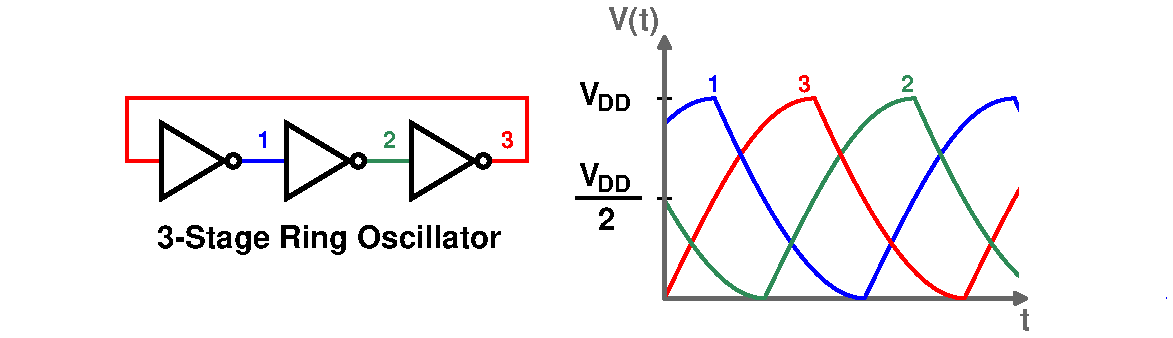
\includegraphics[width=0.8\linewidth, angle=0]{figs/theory/osc_waves}
			\caption{Model for ring oscillator.}
			\label{fig:rosc_rc}
		\end{figure}

		\begin{figure}[htb!]
	        \centering
	        \begin{subfigure}{.5\textwidth}
	            \centering
	            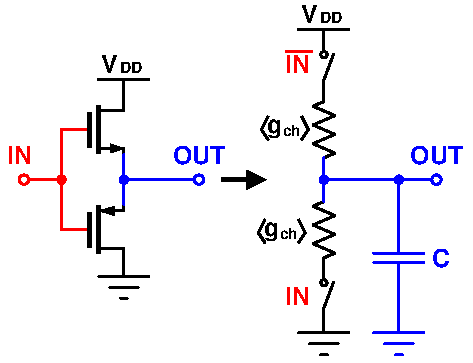
\includegraphics[width=\linewidth]{figs/design/inv_rc_model}
	            \caption{Inverter approximate model.}
	            \label{fig:inv_cir}
	        \end{subfigure}%
	        \begin{subfigure}{.5\textwidth}
	            \centering
	            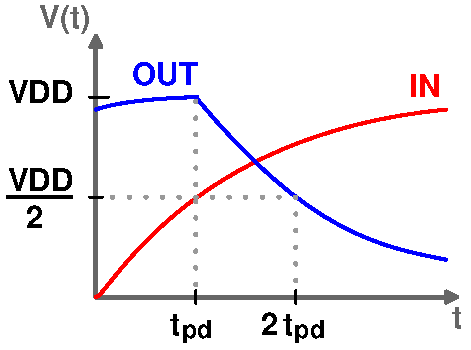
\includegraphics[width=0.8\linewidth]{figs/design/inv_waves}
	            \caption{Inverter waveforms in ring oscillator.}
	            \label{fig:inv_wave}
	        \end{subfigure}
	        \caption{Approximate model for ring oscillator inverter delay cell.}
	        \label{fig:inv_model}
	    \end{figure}

		To calculate oscillation frequency ring oscillator from the RC model, several inferences are made:
		\begin{itemize}
			\item The switching point $V_M$ of the inverters is $V_{DD}/2$, based on the assumption that the NMOS and PMOS are of equal strength.
			\item The output of an inverter will have a decaying exponential which starts coincident with the passing of $V_M$ at the input.
			\item The propagation delay $t_{pd}$ for an inverter will be the time differential between the $V_M$ crossing points on the input and output.
			\item The oscillator frequency will be $f_{osc}$ = $1/2Nt_{pd}$, where N is the number of stages (i.e. defined by 2N propagation delays).
		\end{itemize}
			Given the falling edge inverter waveform equation in \ref{eq:inv_exp}, and observing that $t_{pd}$ occurs at the point where $V(t) = V_{DD}/2$, it is found that $t_{pd}$ = $\tau\ln(2)$. Finally, using the aforementioned assumptions, the equation for oscillator frequency in equation \ref{eq:ro_osc_freq}.

			\begin{equation}\label{eq:inv_exp}
			V(t) = V_{DD}\cdot e^{\frac{-t}{\tau}}\cdot u(t)
			\end{equation}

			\begin{equation}\label{eq:ro_osc_freq}
				f_{osc}^{-1} = 2Nt_{pd} = \frac{2\ln(2)NC}{\langle g_{ch}\rangle}
			\end{equation}


		\subsubsection{Finding $\langle g_{ch}\rangle$ and C}
			The node capacitance C is trivial to find based on the inverter gate capacitance and a lumped load capacitance term $C_L$:
			\begin{equation}
				C = C_{ox}\left ( W_N L_N + W_P L_N \right) + C_L
			\end{equation}
			The average channel conductance $\langle g_{ch} \rangle$ is more involved to find. To do so, several assumptions are made:
			\begin{itemize}
				\item L $>>$ L$_{min}$, so no velocity saturation, and therefore square law is applicable.
				\item NMOS and PMOS have equal $V_{TH}$ and transconducance.
				\item Output transition occur with the active FET in saturation from the start of the transition until $t_{pd}$ after the start of the transition. This requires:
				\begin{itemize}
					\item $V_{DD}/4 < V_{TH} < V_{DD}/2$
				\end{itemize}
			\end{itemize}
			Following those assumptions, $\langle g_{ch} \rangle$ can be computed via integral within the period $t_{pd}$:
			\begin{equation}
				\langle g_{ch} \rangle = \frac{1}{t_{pd}} \int_0^{t_{pd}}\frac{I_{out}(t)}{V_{out}(t)}dt
			\end{equation}
			$I_{out}$ is computed using the saturated MOSFET square law model an exponential waveforms assumptions. An $I_{short}$ term is included to account for output current reduction from short-circuit conduction when both PMOS and NMOS are conducting.
			\begin{align}
				I_{out}(t) &= \frac{k_n}{2}\left(\frac{W}{L}\right)_n\left[\left(V_{in}(t) - V_{TH}\right)^2 \right]  - I_{short} \\
				&= \frac{k_n}{2}\left(\frac{W}{L}\right)_n \left[\left(V_{DD}\left(1-e^{-t/\tau}\right) - V_{TH}\right)^2 - \left(\frac{V_{DD}}{2} -V_{TH}\right)^2\right]
			\end{align}
			$k_n = \mu_nC_{ox}$, with the equal PMOS/NMOS assumption, $k_n\left(\frac{W}{L}\right)_n=k_p\left(\frac{W}{L}\right)_p$. $V_{out}$ is simply a decaying exponential with a delay $t_{pd}$ versus the input:
			\begin{equation}
				V_{out} = V_{DD}e^{-(t-t_{pd})/\tau}
			\end{equation}
			Now, computing the integral for $\langle g_{ch} \rangle$ yields:
			\begin{equation}
				\langle g_{ch} \rangle = \frac{1}{2}\mu_nC_{ox}\left(\frac{W}{L}\right)_n\left[V_{DD}\left(\frac{7}{8\ln2}-1\right)-V_{TH}\left(\frac{1}{\ln2}-1\right) \right]
			\end{equation}
			As a simplification, $\alpha$ is defined as:
			\begin{equation}
				\alpha = \left[V_{DD}\left(\frac{7}{8\ln2}-1\right)-V_{TH}\left(\frac{1}{\ln2}-1\right) \right]
			\end{equation}	
		
		\subsubsection{Handling unequal NMOS/PMOS}
			In the case of different threshold voltages for NMOS and PMOS:
			\begin{equation}
				f_{osc}^{-1} = N(t_{pdn} + t_{pdp}) = \ln(2)NC\left(\frac{1}{\langle g_{ch}\rangle_n} + \frac{1}{\langle g_{ch}\rangle_p}\right) = \frac{2\ln(2)NC}{\langle g_{ch}\rangle'}
			\end{equation}	
			A modified $\langle g_{ch}\rangle'$ is defined:
			\begin{align}
				\langle g_{ch}\rangle' = 2\left(\frac{1}{\langle g_{ch}\rangle_n} + \frac{1}{\langle g_{ch}\rangle_p}\right)^{-1} = 2\frac{\langle g_{ch}\rangle_n \langle g_{ch}\rangle_p}{\langle g_{ch}\rangle_n + \langle g_{ch}\rangle_p}
				= 2\frac{\frac{1}{2}\mu_nC_{ox}\left(\frac{W}{L}\right)_n \alpha_n\frac{1}{2}\mu_pC_{ox}\left(\frac{W}{L}\right)_p \alpha_p}{\frac{1}{2}\mu_nC_{ox}\left(\frac{W}{L}\right)_n\alpha_n + \frac{1}{2}\mu_pC_{ox}\left(\frac{W}{L}\right)_p\alpha_p}
			\end{align}	
			This is somewhat unmanagable, however enforcing $\mu_nC_{ox}\left(\frac{W}{L}\right)_n = \mu_pC_{ox}\left(\frac{W}{L}\right)_p$ for $V_M$ to equal $V_{DD}/2$ gives:
			\begin{align}
				\langle g_{ch}\rangle' = \frac{1}{2}\mu_nC_{ox}\left(\frac{W}{L}\right)_n\frac{2 \alpha_n\alpha_p}{\alpha_n + \alpha_p} = \frac{1}{2}\mu_nC_{ox}\left(\frac{W}{L}\right)_n \alpha'
			\end{align}	
			Thus $\alpha_n$ and $\alpha_p$ are found for the according threshold voltages and then $\langle g_{ch}\rangle$ can be found.
			\begin{equation}
				\alpha' =  \frac{2 \alpha_n\alpha_p}{\alpha_n + \alpha_p}
			\end{equation}

		\subsubsection{Solving for oscillator frequency and power}
			Solving for oscillator frequency:
			\begin{equation}
				f_{osc} = \frac{\mu_nC_{ox}}{4\ln2NC}\left(\frac{W}{L}\right)_n\left[V_{DD}\left(\frac{7}{8\ln2}-1\right)-V_{TH}\left(\frac{1}{\ln2}-1\right) \right]
			\end{equation}
			If gate capacitance is the dominant load component, and PMOS/NMOS are equal sized such that $C=2WLC_{ox}$:
			\begin{equation}
				f_{osc} = \frac{\mu_n}{8\ln2N}\cdot\frac{1}{L^2}\left[V_{DD}\left(\frac{7}{8\ln2}-1\right)-V_{TH}\left(\frac{1}{\ln2}-1\right) \right]
			\end{equation}
			Power can also be calculated, knowing in digital circuits $P = fC_{\Sigma}V_{DD}^2$, where $C_{\Sigma}$ is the total capacitance of the active nodes. Thus:
			\begin{equation}
				P_{osc} = Nf_{osc}CV_{DD}^2 = \frac{\mu_nC_{ox}}{4\ln2}\left(\frac{W}{L}\right)_n\left[V_{DD}\left(\frac{7}{8\ln2}-1\right)-V_{TH}\left(\frac{1}{\ln2}-1\right) \right]
			\end{equation}
			It should be noted that the power consumption is proportional to FET aspect ratio (W/L), regardless of the load.

	\subsubsection{Ring oscillator backgate tuning derivation}
		Using the basic expressions for ring oscillator frequency, the operature under backgate biasing can be found. In FD-SOI, the threshold voltage of a FET varies with linear dependence on the applied back gate bias $V_{BG}$ (relative to source). Given the body effect coefficient of a process, $\gamma$, $V_t$ is:
		\begin{equation}
			V_{TH} = V_{t0} - \gamma V_{BG}
		\end{equation}
		Using this in the ring oscillator frequency equation:
		\begin{equation}
			f_{osc} = \frac{\mu_nC_{ox}}{4\ln2NC}\left(\frac{W}{L}\right)_n\left[V_{DD}\left(\frac{7}{8\ln2}-1\right)-V_{t0}\left(\frac{1}{\ln2}-1\right) + \gamma V_{BG}\left(\frac{1}{\ln2}-1\right) \right]
		\end{equation}
		Equivalently, $f_{osc} = f_{0,osc} + \Delta f_{osc}(V_{BG})$, provided $f_{0,osc}$ is the frequency with no backgate bias where. Thus it is found that:
		\begin{equation}\label{eq:kvco_}
			\Delta f_{osc}(V_{BG}) = \gamma V_{BG}\frac{\mu_nC_{ox}}{4\ln2NC}\left(\frac{W}{L}\right)_n\left[\frac{1}{\ln2}-1\right] = K_{VCO}
		\end{equation}	

		The important finding here is that the change in oscillator frequency is linear with backgate voltage, that is $\Delta f_{osc} \propto V_{BG}$. The expression of \ref{eq:kvco_} also happens to to be the oscillator VCO gain, $K_{VCO}$. Given the wide voltage range that FD-SOI backgates may be biased to, this implies that a highly linear VCO with wide input range may be implemented with backgate tuning. If the backgate voltage is constrained in the range [0, $V_{DD}$], the center frequency $f_c$ of such a VCO is then:
		\begin{equation}
			f_{c} = \frac{\mu_nC_{ox}}{4\ln2NC}\left(\frac{W}{L}\right)_n\left[V_{DD}\left(\frac{7}{8\ln2}-1+\frac{\gamma}{2\ln2}-\frac{\gamma}{2}\right)-V_{t0}\left(\frac{1}{\ln2}-1\right)\right]
		\end{equation}
		Correspondingly, the tuning range with $V_{BG} \in$ [0, $V_{DD}$] is:
		\begin{equation}\label{eq:tuning_range}
			\Delta f = \gamma V_{DD}\frac{\mu_nC_{ox}}{4\ln2NC}\left(\frac{W}{L}\right)_n\left[\frac{1}{\ln2}-1\right]
		\end{equation}
		Finally, the fractional tuning range of the oscillator found to be that of equation \ref{eq:frac_range}. Notice that this is only a function of supply voltage $V_{DD}$, nominal threshold voltage $V_{t0}$ and body effect coefficient $\gamma$.
		\begin{equation}\label{eq:frac_range}
			\frac{\Delta f}{f_c} = \frac{\gamma V_{DD}\left( 1-\ln2 \right)}{V_{DD}\left(\frac{7}{8}-\ln2+\frac{\gamma}{2}-\frac{\gamma}{2}\ln2\right)-V_{t0}\left(1-\ln2\right)}
		\end{equation}	
		If a N-bit DAC is used to control the oscillator, the resulting DCO gain is therefore:
		\begin{equation}
			K_{DCO} = \frac{\Delta f}{2^{N_{DAC}}} = \frac{f_c}{2^{N_{DAC}}}\cdot\frac{\gamma V_{DD}\left( 1-\ln2 \right)}{V_{DD}\left(\frac{7}{8}-\ln2+\frac{\gamma}{2}-\frac{\gamma}{2}\ln2\right)-V_{t0}\left(1-\ln2\right)}
		\end{equation}	
	\subsubsection{DCO Gain Uncertainty}
		The DCO gain $K_{DCO}$ is used in setting the loop filter coefficients, so the uncertainty of the DCO gain is of interest to allow for statistical analysis of the PLL across process variation. The uncertainty of $K_{DCO}$ (normalized with nominal $K_{DCO}$ value) as a function of $V_{DD}$, $V_{t0}$ and $\gamma$ is:
		\begin{equation}
			\sigma_{KDCO} = \sqrt{\left(\frac{\partial K_{DCO}}{\partial V_{DD}}\cdot\frac{\sigma_{VDD}}{K_{DCO}} \right)^2 + \left(\frac{\partial K_{DCO}}{\partial V_{t0}}\cdot\frac{\sigma_{Vt0}}{K_{DCO}} \right)^2 + \left(\frac{\partial K_{DCO}}{\partial \gamma}\cdot\frac{\sigma_\gamma}{K_{DCO}} \right)^2}
		\end{equation}

		\begin{align}
			\frac{\partial K_{DCO}}{\partial V_{DD}} &= \frac{f_c}{2^{N_{DAC}+1}}\cdot\frac{-\gamma V_{t0}(1-\ln2)^2}{\left[ V_{DD}\left(\frac{7}{8}-\ln2+\frac{\gamma}{2}-\frac{\gamma}{2}\ln2\right)-V_{t0}\left(1-\ln2\right) \right]^2}\\
			\frac{\partial K_{DCO}}{\partial V_{t0}} &= \frac{f_c}{2^{N_{DAC}+1}}\cdot\frac{\gamma V_{DD}(1-\ln2)^2}{\left[ V_{DD}\left(\frac{7}{8}-\ln2+\frac{\gamma}{2}-\frac{\gamma}{2}\ln2\right)-V_{t0}\left(1-\ln2\right) \right]^2}\\
			\frac{\partial K_{DCO}}{\partial \gamma} &= \frac{f_c}{2^{N_{DAC}+1}}\cdot\frac{V_{DD}\cdot(1-\ln2) \left[ V_{DD}\left(\frac{7}{8}-\ln2\right)-V_{t0}\left(1-\ln2\right) \right]}{\left[ V_{DD}\left(\frac{7}{8}-\ln2+\frac{\gamma}{2}-\frac{\gamma}{2}\ln2\right)-V_{t0}\left(1-\ln2\right) \right]^2}
		\end{align}
		Simplified:
		\begin{multline}
			\sigma_{KDCO} = \frac{1}{\gamma V_{DD} \left[ V_{DD}\left(\frac{7}{8}-\ln2+\frac{\gamma}{2}-\frac{\gamma}{2}\ln2\right)-V_{t0}\left(1-\ln2\right) \right]}\cdot\\ \sqrt{\left(\gamma V_{t0} (1-\ln2)\sigma_{VDD} \right)^2 + \left(\gamma V_{DD} (1-\ln2)\sigma_{Vt0} \right)^2 + \left( V_{DD}\left[ V_{DD}\left(\frac{7}{8}-\ln2\right)-V_{t0}\left(1-\ln2\right) \right]\sigma_{\gamma} \right)^2 }
		\end{multline}	

		% \hl{Motivate selection of fine backgate tuning and supply coarse tuning (as future extension?). I.e. what is df/dVdd vs df/dVbg?}
		% \hl{\textbf{TODO} - extract $\gamma$, $V_{t0}$ variance for FETs in process kit, place in results?}

		\subsubsection{Backgate-controlled Ring Oscillator Sensitivity Analysis}
		The frequency tuning sensitivity of the ring oscillator for supply and backgate voltages will be compared. First the following is defined, following that the derived equations for oscillator frequency are linear.
		\begin{equation}
			f_{osc}(V_{DD}+\Delta V_{DD}) = f_{osc}(V_{DD}) + f_{osc}(\Delta V_{DD})
		\end{equation}
		\begin{equation}
			f_{osc}(V_{DD}) = f_0
		\end{equation}
		\begin{equation}
			f_{osc}(\Delta V_{DD}) = \Delta f
		\end{equation}

		In the case of supply voltage tuning, the change (proportion) of frequency per voltage of applied extra bias is (evaluated at zero back-gate bias):
		\begin{equation}
			S^{f_{osc}}_{V_{DD}} = \frac{\Delta f}{f_0}\cdot\frac{1}{\Delta V_{DD}}  = \frac{\left(\frac{7}{8\ln2}-1\right)}{V_{DD}\left(\frac{7}{8\ln2}-1\right)-V_{t0}\left(\frac{1}{\ln2}-1\right)}
		\end{equation}
		With $V_{DD}$ = 0.8, $V_{t0}$ = 0.3 (approximately true for 22FDX devices), it is expected 340\% change in frequency will result per extra volt of applied bias. Of course, this is linearized, and one does not expect to apply an extra 1V of supply bias to a 0.8V oscillator. Realistically, the supply can be tuned $\pm$ 10\%, which corresponds to a $\pm$27.2\% tuning range of the oscillator. Supply tuning stands as a viable coarse tuning mechanism for the oscillator, however, fine tuning is more limited due to difficulty in achieving small resolution step (e.g 10 bits in $V_{DD}$ = 0.8V $\pm$10\% corresponds to 156 $\mu$V/LSB, and 26 m\%/LSB of frequency tuning).

		\par In the case of backgate tuning, the change (proportion) of frequency per volt of applied backgate bias is:
		\begin{equation}
			S^{f_{osc}}_{V_{BG}} = \frac{\Delta f}{f_0}\cdot\frac{1}{\Delta V_{BG}}  = \frac{\gamma \left(\frac{1}{\ln2}-1\right)}{V_{DD}\left(\frac{7}{8\ln2}-1\right)-V_{t0}\left(\frac{1}{\ln2}-1\right)}
		\end{equation}

		With $\gamma$=0.07, $V_{DD}$=0.8, $V_{t0}$=0.3, as is typical in 22FDX, it is expected a 29.5\% change in frequency will result per volt applied of backgate bias. This is much finer than achieved with supply voltage tuning. The ratio of frequency sensitivity to supply and backgate voltage tuning is:

		\begin{equation}
			\frac{S^{f_{osc}}_{V_{DD}}}{S^{f_{osc}}_{V_{BG}}} =  \frac{\frac{7}{8\ln2}-1}{\gamma \left(\frac{1}{\ln2}-1\right)}
		\end{equation}
		Under the aforementioned biasing conditions, it is expected that 8.4x finer control can be achieved with backgate tuning. The wide backgate voltage ranges allowed for with FD-SOI technology permit for design of a voltage-DAC based controll scheme which will achieve far smaller frequency resolution than with supply voltage tuning. 

		\subsubsection{Capacitor-based coase tuning scheme}
		It is observed that oscillator frequency of ring oscillator is capacitance dependent. Thus if a bank of quantized capacitances may be switched into the oscillator, coarse control of frequecy can be implemented. Figure \ref{fig:rosc_tuning} demonstrates the effect of such a tuning scheme, for increasing capacitance settings C0-C3. Under such a scheme it is important to ensure that the frequency ranges acheived through backgate tuning overlap between sucessive capacitor settings to ensure continuity of frequencies accessible by the oscillator. 
		\FloatBarrier
		\begin{figure}[htb!]
			\center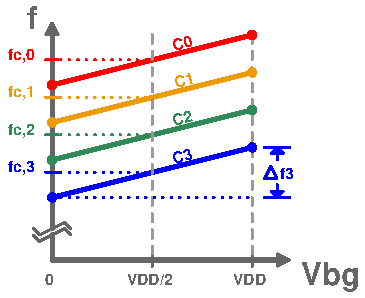
\includegraphics[width=0.4\linewidth, angle=0]{figs/backgate_rosc_tuning2.pdf}
			\caption{Backgate-tuned ring oscillator with coarse tuning capacitor bank.}
			\label{fig:rosc_tuning}
		\end{figure}

%%%%%%%%%%%%%%%%%%%%%%%%%%%%%%%
		
		\FloatBarrier\pagebreak
		\subsubsection{Pseudodifferential Backgate-Coupled Inverter Delay Cell}\label{sec:pd_inv}
		To utilize backgate tuning for frequency control, a suitable delay cell design must be devised. Accordingly, the delay topology used in this work has been derived from the FD-SOI pseudodifferential backgate coupled inverter delay cell of \cite{Jacquemod2019}, shown in figure \ref{fig:bg_inv_jacqu}. This inverter uses two single ended FD-SOI inverters, with the backgates of the transistors in a given inverter connected together. This is implemented with a common well structure below the two transistors of each inverter. Nominally, to avoid forward biasing of the well-substrate diodes, a N-doped well or a triple well is used, with well potentials constrained to be $\geq$ 0. The result of this well configuration and the FD-SOI BOX layer is that the backgate terminals of the PMOS and NMOS may be tuned in tandem across a wide positive voltage range. This is not possible in bulk technology. In 22FDX, such well configurations allow biasing from 0 to +2V, which is inclusive of the full rail-to-rail range of a circuit supplied with $V_{DD}$ = 0.8V, as in this work. Thus, in figure \ref{fig:bg_inv_jacqu}, when the two FD-SOI sub-cells inverter cells connected with the shown cross-coupled output and backgate configuration, safe well biasing is achieved. The backgate cross-coupled configuration has the effect of inducing differential behavior in the circuit, as positive feedback is introduced. It should be noted that cell of figure \ref{fig:bg_inv_jacqu} does not employ back gate tuning to tune frequency. This work proposes a modification to the topology which implements backgate differential coupling and backgate frequency tuning.

		\begin{figure}[htb!]
		        \centering
		        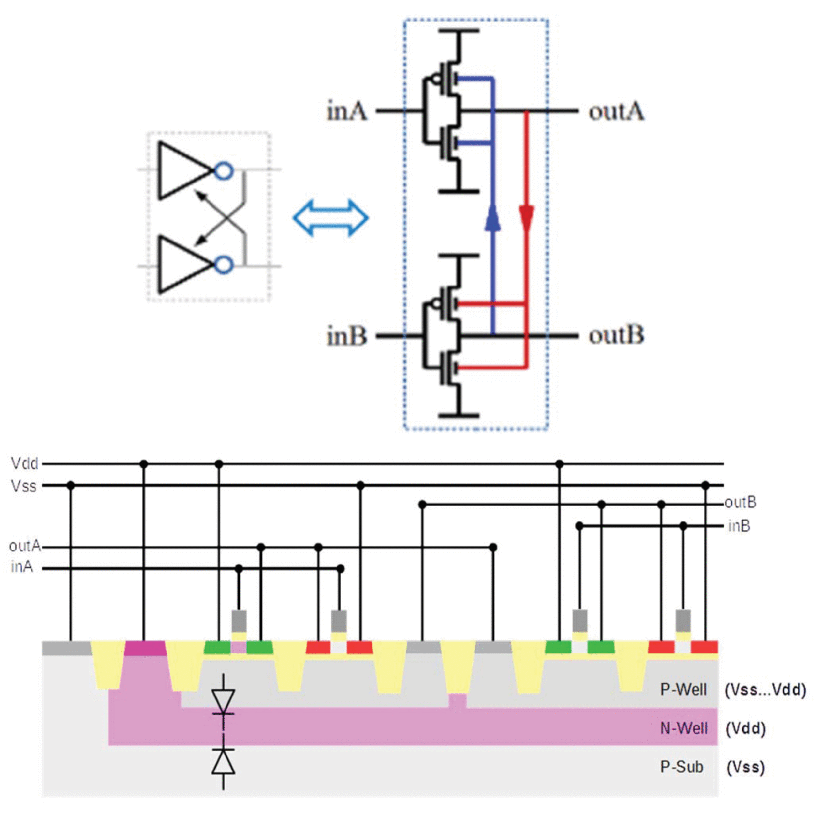
\includegraphics[width=0.58\textwidth, angle=0]{./figs/design/jacqu2-1-large.png}
		    \caption{FD-SOI backgate-coupled inverter topology, .}
		    \label{fig:bg_inv_jacqu}
		\end{figure}	

		The emergence of differential behavior in this delay cell can be understood through circuit analysis. First, the common backgate inverter cell (figure \ref{fig:fig_10a}) is converted to a linearized model, for an arbitrary bias point, in figure \ref{fig:fig_10b}. A simplification of the linearized model is arrived at by lumping terms together, giving figure \ref{fig:fig_10c}. Using the linearized model of figure \ref{fig:fig_10c}, a linearized version of the pseudodifferential inverter circuit is then arrived at in figures \ref{fig:pseudodiff_cir} and \ref{fig:pseudodiff_linearized}. It is observed that transconductors $-G_{mb}$ in figure \ref{fig:pseudodiff_linearized} couple the two outputs with positive feedback loop. Therefore, any differential components generated via the feed forward terms $-G_m R_o v_{in}$ and $-G_m R_o v_{ip}$ will be positively amplified by the cross coupling. Elementary circuit analysis for differential gain of the linear circuit in figure \ref{fig:pseudodiff_linearized} leads to the expression in equation \ref{eq:pd_dm_gain}.

			\begin{figure}[htb!]
			    \centering
			    \begin{subfigure}{0.33\textwidth}
			        \centering
			        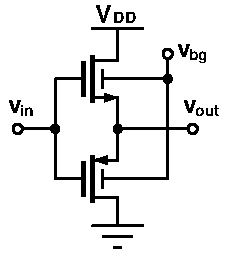
\includegraphics[width=1\textwidth, angle=0]{./figs/design/fig_10a_}
			        \caption{ }
			        \label{fig:fig_10a}
			    \end{subfigure}%
			    \begin{subfigure}{0.33\textwidth}
			        \centering
			        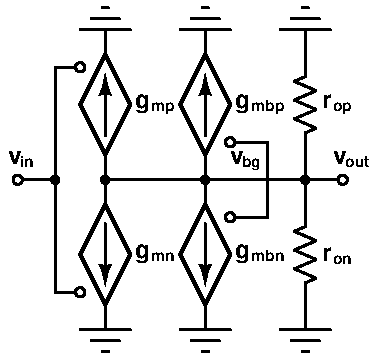
\includegraphics[width=1\textwidth, angle=0]{./figs/design/fig_10b}
			        \caption{ }
			        \label{fig:fig_10b}
			    \end{subfigure}
			    \begin{subfigure}{0.33\textwidth}
			        \centering
			        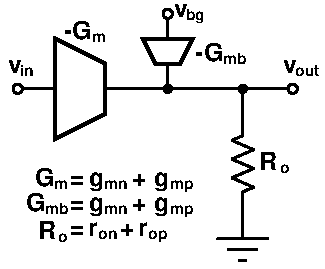
\includegraphics[width=1\textwidth, angle=0]{./figs/design/fig_10c}
			        \caption{ }
			        \label{fig:fig_10c}
			    \end{subfigure}
			    % \caption{x.}
			    \caption{\textbf{(a)} Common backgate inverter, \textbf{(b)} Linearized circuit, \textbf{(c)} Simplified linearized model.}
			    \label{fig:bg_inv_model}
			\end{figure} 

			\begin{figure}[htb!]
			    \centering
			    \begin{subfigure}{0.3\textwidth}
			        \centering
			        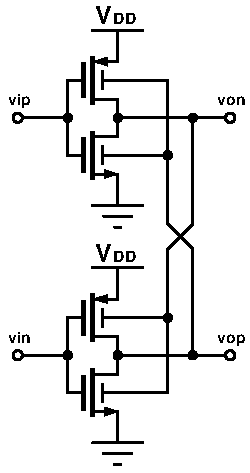
\includegraphics[width=1\textwidth, angle=0]{./figs/design/pseudodiff_bw}
			        \caption{ }
			        \label{fig:pseudodiff_cir}
			    \end{subfigure}%
			    \hspace{5em}
			    \begin{subfigure}{0.35\textwidth}
			        \centering
			        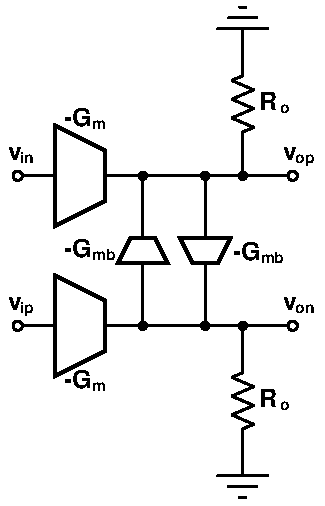
\includegraphics[width=1\textwidth, angle=0]{./figs/design/pseudodiff_buff_linear}
			        \caption{ }
			        \label{fig:pseudodiff_linearized}
			    \end{subfigure}
			    % \caption{x.}
			    \caption{\textbf{(a)} Pseudodifferential backgate-coupled inverter circuit, \textbf{(b)} Linearized circuit.}
			    \label{fig:pd_cir_inv_model}
			\end{figure} 

			\begin{equation}\label{eq:pd_dm_gain}
				A_{DM} = \frac{G_mR_o + G_{mb}^2R_o^2}{1 - G_{mb}^2R_o^2}
			\end{equation}
			Using the relation $G_{mb} = \gamma G_{m}$ found in equation \ref{eq:gm_gmb_relation}, equation \ref{eq:pd_dm_gain} can be simplified to \ref{eq:pd_dm_gain2} (this is assuming PMOS and NMOS have approximately equal $\gamma$). In the special case where $\gamma G_mR_o \approx 1$, the differential gain of the delay cell can be very high, implying the pseudodifferential coupling can be very effective at inducing differential behavior. A major advantage of this topology is that it is implemented using only two inverters, unlike typical differential pair circuits which rely on current biasing to achieve differential behavior. The removal of the need for current biasing reduces power consumption, as no bias generators are required. Circuit noise is also reduced due to fewer total transistors generating noise in the circuit.
			\begin{equation}\label{eq:pd_dm_gain2}
				A_{DM} = \frac{G_mR_o }{1 - \gamma G_mR_o }
			\end{equation}
			For the sake of completeness, the common mode gain of the circuit has also been determined by the same method, given in equation \ref{eq:pd_cm_gain}.
			\begin{equation}\label{eq:pd_cm_gain}
				A_{CM} = \frac{G_mR_o }{1 + \gamma G_mR_o }
			\end{equation}

%%%%%%%%%%%%%%%%%%%%%%%%%%%%%%%%%%%%%%%%%%%%%%%%%%%%%%%%%%%%%%%%%%%%%%%%%%%

			\FloatBarrier\subsubsection{Tunable Frequency Backgate-Coupled Pseudodifferential Delay Cell}
			To implement the backgate-coupled pseudo-differential inverter delay cell topology with backgate tuning, two cantidate topologies have been devised. The first is the parallel cofigured topology of figure \ref{fig:parallel_delay_cell}, and the second is a telescopic configutation, shown in figure \ref{fig:telescopic_delay_cell}.

			\begin{figure}[htb!]
			    \centering
			    \begin{subfigure}{0.5\textwidth}
			        \centering
			        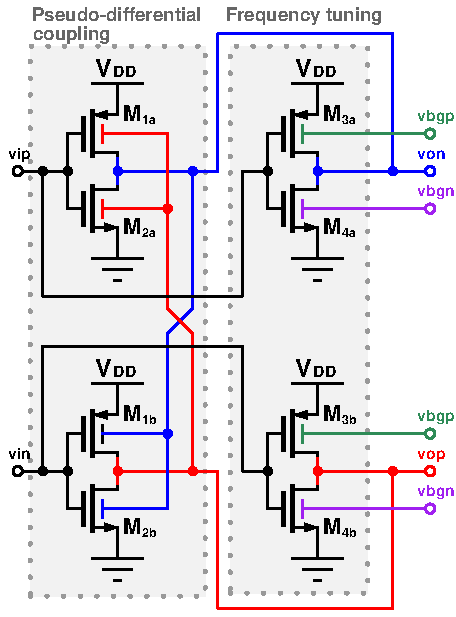
\includegraphics[width=1\textwidth, angle=0]{./figs/design/parallel_delay_cell2}
			        \caption{ }
			        \label{fig:parallel_delay_cell}
			    \end{subfigure}%
			    \begin{subfigure}{0.5\textwidth}
			        \centering
			        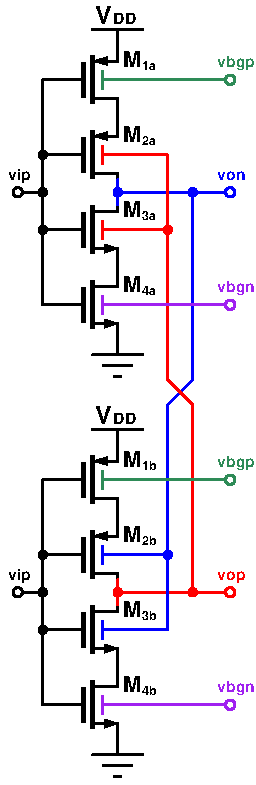
\includegraphics[height=0.5\textheight, angle=0]{./figs/design/tele_delay_cell2}
			        \caption{ }
			        \label{fig:telescopic_delay_cell}
			    \end{subfigure}
			    % \caption{x.}
			    \label{fig:tunable_delay_cells}
			    \caption{Backgate tunable backgate-coupled pseudodifferential delay cell in\textbf{(a)} Parallel, \textbf{(b)} Telescopic implementations.}
			\end{figure} 


			The parallel cofigured topology employs backgate-coupled pseudo-differential inverter in parallel with a second set of inverters, which the backgate voltages are set externally to control the oscillator frequency. 


			The telecopic topology is comprised of two sub-inverters each with a telescopic stack of four transistors. The header and footer transistor backgates are connected to external control voltages to adjust frequency. Modulating the control voltages will modulate the conductance of the header and footer devices, which result in a current-starving like behavior that modulate oscillator frequency. The inner pair of transistors in each sub-inverter are configured with a common backgate, which are cross-coupled with the output of the other respective sub-inverter, to induce differential operation in the same manner as the basic backgate-coupled pseudo-differential inverter delay cell. 

			Hajimiri's oscillator impulse sensitivity function (ISF) paper \cite{Hajimiri1998} suggests that it is favorable for an oscillator to have as symmetric rise and fall time. Higher symmetry of waveform results in a lower corner frequency for flicker noise, thus low frequency phase noise will be improved.



			\begin{figure}[htb!]
			    \centering
			    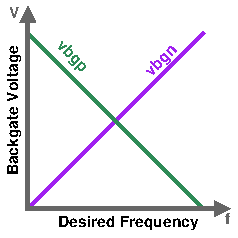
\includegraphics[width=0.4\textwidth, angle=0]{./figs/design/tuning}
			    \caption{Complementary tuning of backgate voltages to achieve frequency tuning.}
			    \label{fig:bg_tuning_scheme}
			\end{figure}



			\begin{itemize}[itemsep=4pt,label=\protect---]
				\item Must use devices in N well (PFET, HVTPFET, SLVTNFET, LVTNFET) to not forward bias substrate diode.
				\item To achieve $V_{m}$ =  $V_{DD}/2$, PFET + LVTNFET give most reasonable W$_P$/W$_N$, ca 1.2-1.4.
				\begin{itemize}[itemsep=4pt,label=$\bullet$]
					\item SLVTNFET + PFET needs W$_P$/W$_N$ $\approx$ 8.
				\end{itemize}
			\end{itemize}


			\begin{figure}[htb!]
			    \centering
			    \begin{subfigure}{0.5\textwidth}
			        \centering
			        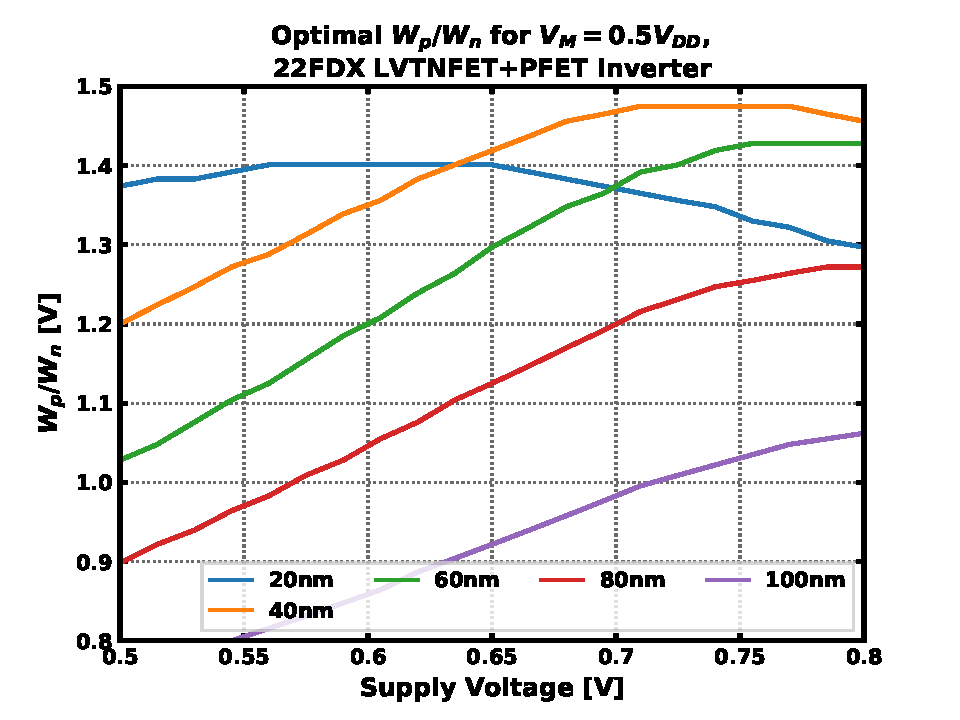
\includegraphics[width=1\textwidth, angle=0]{./figs/design/ratio_lvtnfet_pfet}
			        \caption{ }
			        \label{fig:ratio_lvtn_p}
			    \end{subfigure}%
			    \begin{subfigure}{0.5\textwidth}
			        \centering
			        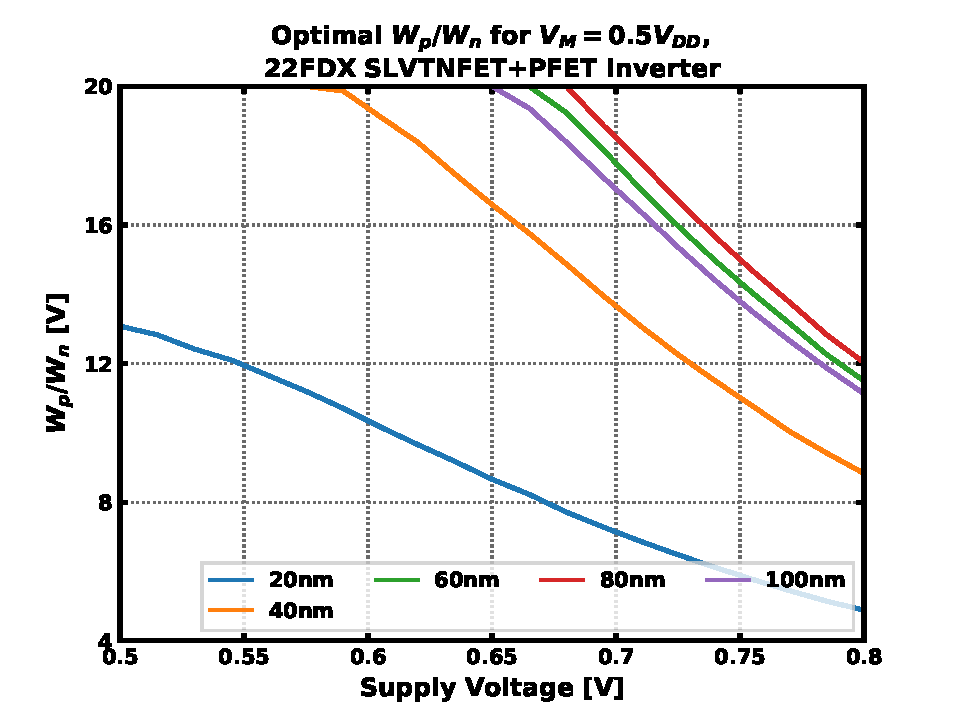
\includegraphics[width=1\textwidth, angle=0]{./figs/design/ratio_slvtnfet_pfet}
			        \caption{ }
			        \label{fig:ratio_slvtn_p}
			    \end{subfigure}
			    % \caption{x.}
			    \label{fig:opt_ratio}
			    \caption{\textbf{(a)} Optimal width PFET/LVTNFET, \textbf{(b)} Optimal width PFET/SLVTNFET.}
			\end{figure} 


			\begin{itemize}[itemsep=4pt,label=\protect---]
				\item Good symmetry of rise time observed, with $V_{cm}$ close to $V_{DD}/2$ over the full oscillation cycle.
				\item \textbf{Observed 10.3\% fractional frequency tuning with L=150nm, FOM=-161 dB, 1:1 ratio of inverters.}
				\item I require $<$ 1\% fractional tuning range to achieve my $K_{DCO}$ with a 10b DAC, this will not work. The (W/L) becomes large to achieve a high inverter ratio, thus increases power too much.
			\end{itemize}



			\begin{itemize}[itemsep=4pt,label=\protect---]
				\item Modify the pseudo-differential cell to have header/footer transistors with back gate control.
				\begin{itemize}[itemsep=4pt,label=$\bullet$]
					\item Cross-coupled devices force differential operation
					\item Header/footer devices used to adjust frequency.
				\end{itemize}				
				\item Ratioing the size of the header/footer devices to the size of the cross-coupling devices tunes $K_{VCO}$
				\item \textbf{Requires complementary control of backgate voltage for tuning.}
			\end{itemize}



			\begin{itemize}[itemsep=4pt,label=\protect---]
				\item Good symmetry of rise time observed, with $V_{cm}$ close to $V_{DD}/2$ over the full oscillation cycle.
				\item $W_p$/$W_n$ = 1.25. Nominal (W/N)$_n$ = 400n/150n
				\item \textbf{1:1 ratioing: Observed 10.0\% fractional frequency tuning with L=150nm, {\color{red}FOM=-162.6 dB.}}
				\item \textbf{1:2 ratioing (header/footer larger): Observed 4.8\% fractional frequency tuning with L=150nm.}
				\item Still hard to get required $<$ 1\% fractional frequency tuning.
			\end{itemize}

			% \begin{figure}[htb!]
			%         \centering
			%         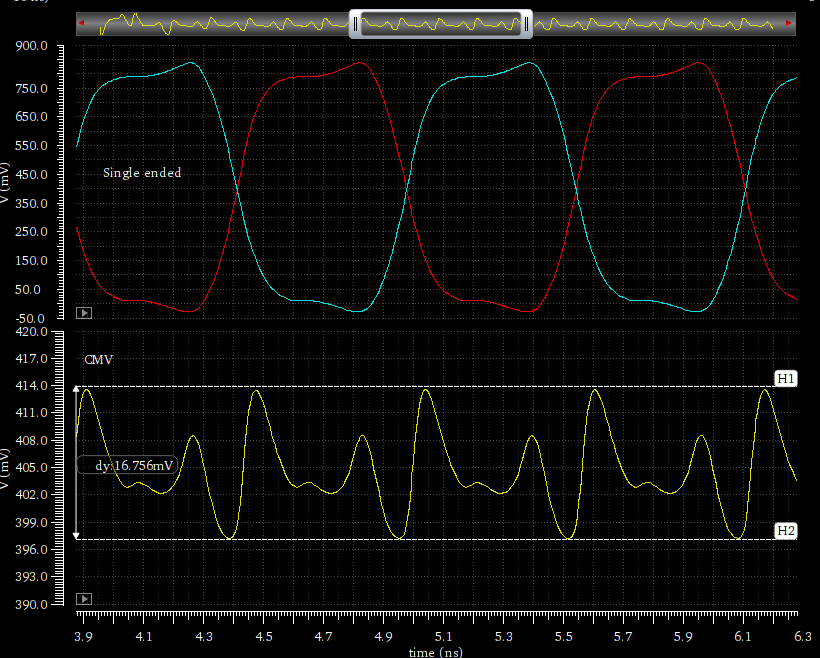
\includegraphics[width=0.8\textwidth, angle=0]{./figs/telescopic_wfm}
			%     % \caption{Approximate model for ring oscillator inverter delay cell.}
			% \end{figure}



			\begin{itemize}[itemsep=4pt,label=\protect---]
				\item Not as linear as I had hoped, $K_{VCO}$ decreases by -33\% when $V_{DD}$ is swept [0, 0.8] V.
				\item I have observed a decease in $\gamma$ at higher back gate biases, this and mobility degredation(??) might explain this trend.
			\end{itemize}



			% \vspace{100em}
			\begin{itemize}[itemsep=4pt,label=\protect---]
				\item PVT (coarse), medium and fine tuning all need to coexist (overlap in frequency).
				\item PVT tuning achieved with bank of differentially connected capacitors
				\item Fine/medium tuning achieved with parallel combination of header/footer transistors. The ratio of these devices affects the difference of the ranges.

			\end{itemize}


			\begin{figure}[htb!]
			        \centering
			        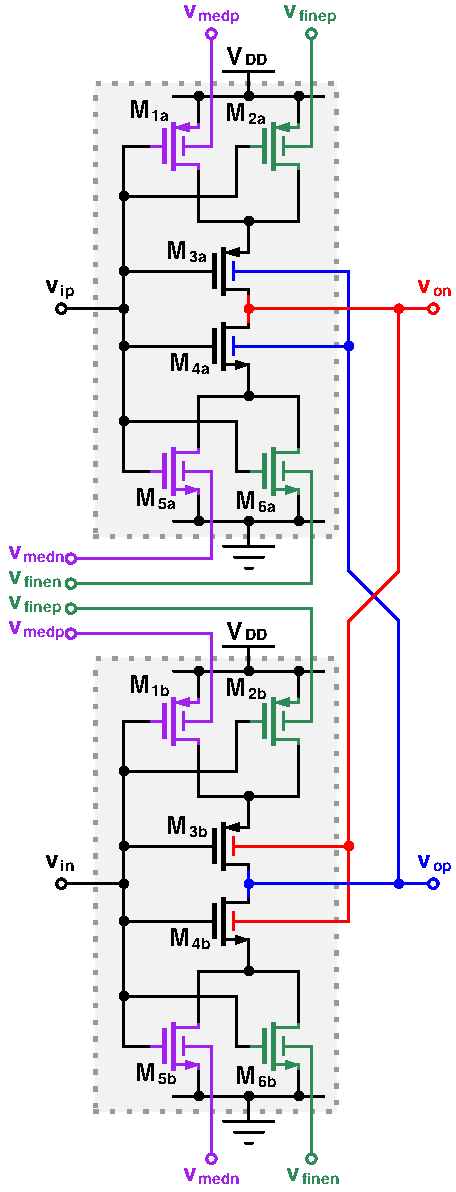
\includegraphics[height=0.6\textheight, angle=0]{./figs/design/delay_cell_pd_inv}
			    \caption{Backgate coupled pseudo-differential inverter delay cell with fine and medium tuning ranges.}
			    \label{fig:pd_delay_cell_fine_med}
			\end{figure}

			\begin{figure}[htb!]
			    \centering
			    \begin{subfigure}{0.5\textwidth}
			        \centering
			        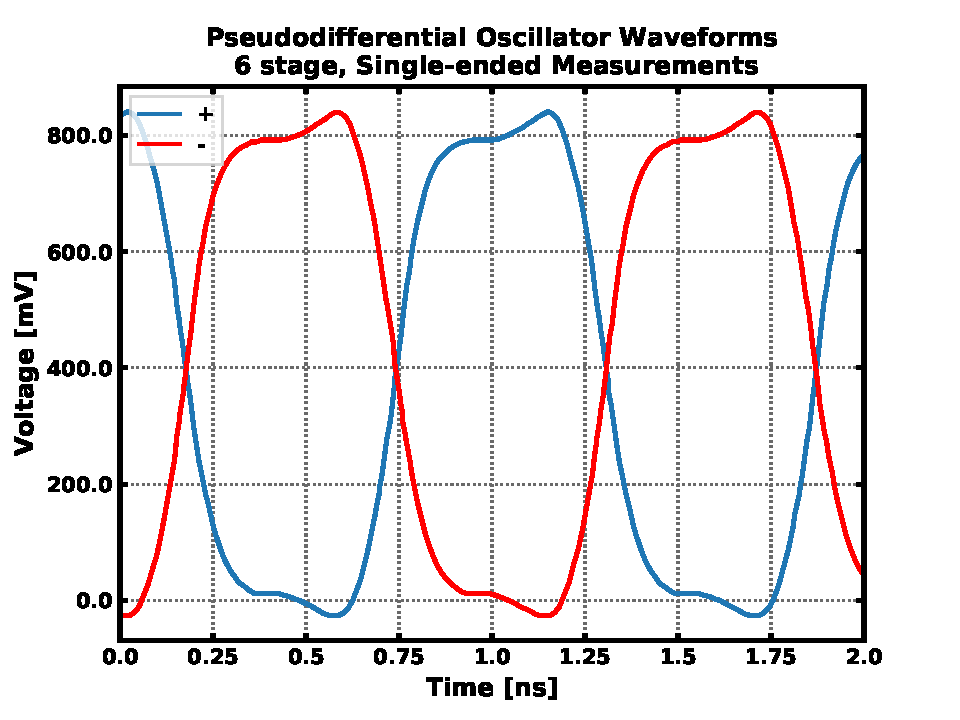
\includegraphics[width=1\textwidth, angle=0]{./figs/results/osc_se_waves}
			        \caption{ }
			        \label{fig:osc_se_waves}
			    \end{subfigure}%
			    \begin{subfigure}{0.5\textwidth}
			        \centering
			        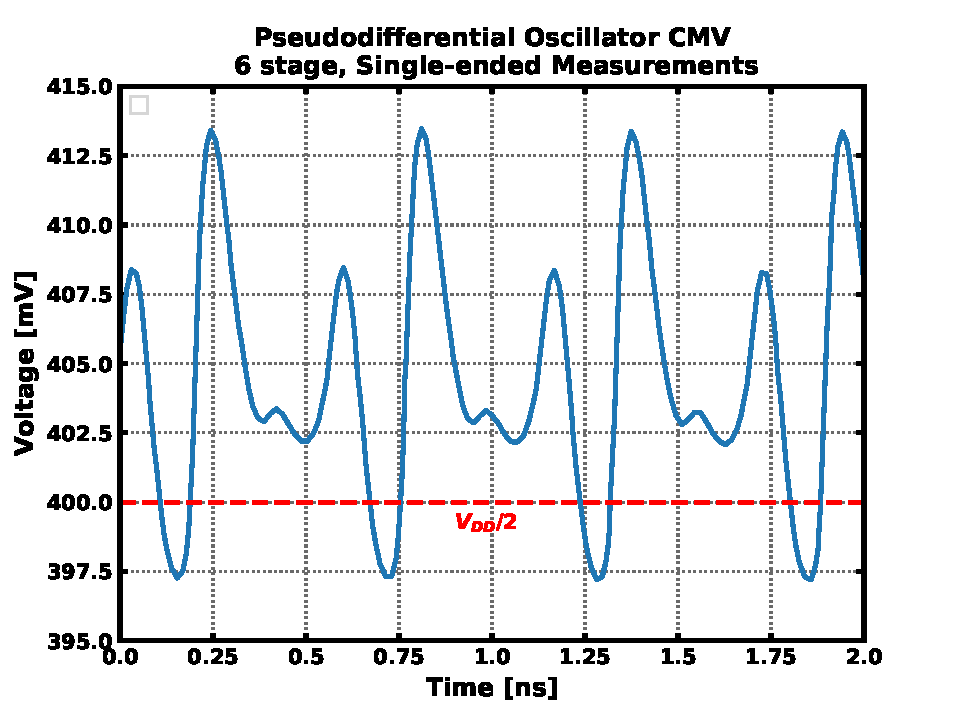
\includegraphics[width=1\textwidth, angle=0]{./figs/results/osc_cmv}
			        \caption{ }
			        \label{fig:osc_cmv}
			    \end{subfigure}
			    % \caption{x.}
			    \caption{\textbf{(a)} Oscillator single-ended waveforms, \textbf{(b)} Oscillator common mode voltage waveform.}
			    \label{fig:osc_waves}
			\end{figure} 


	 Could not get 2 quadrature oscillator stage to oscillate. Period is 4tpd, thus a transition occurs every 2tpd. Propogation delay is ln(2)tau, so a transition every 1.38tau, which equates to enough time to settle to 75\% of the final voltage. Because of partial settling, the oscillation dies in a couple cycles, and is not viable here. To achieve quadrature, 4 stages must be used, however, this was slow to acheive the target 2.448 GHz. Thus, use of sub-harmonic oscillator (show edge combining) due to speed limitations (need short channel length to get right speed, unfortunately phase noise degrades).

		\subsection{Full circuit}
			\begin{figure}[htb!]
			        \centering
			        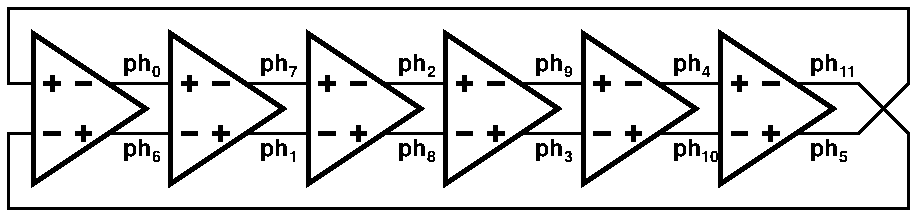
\includegraphics[width=0.8\textwidth, angle=0]{./figs/design/ro_6st_simple}
			    \caption{Basic differential ring oscillator circuit.}
			    \label{fig:basic_6stg_ro}
			\end{figure}
			\begin{figure}[htb!]
			        \centering
			        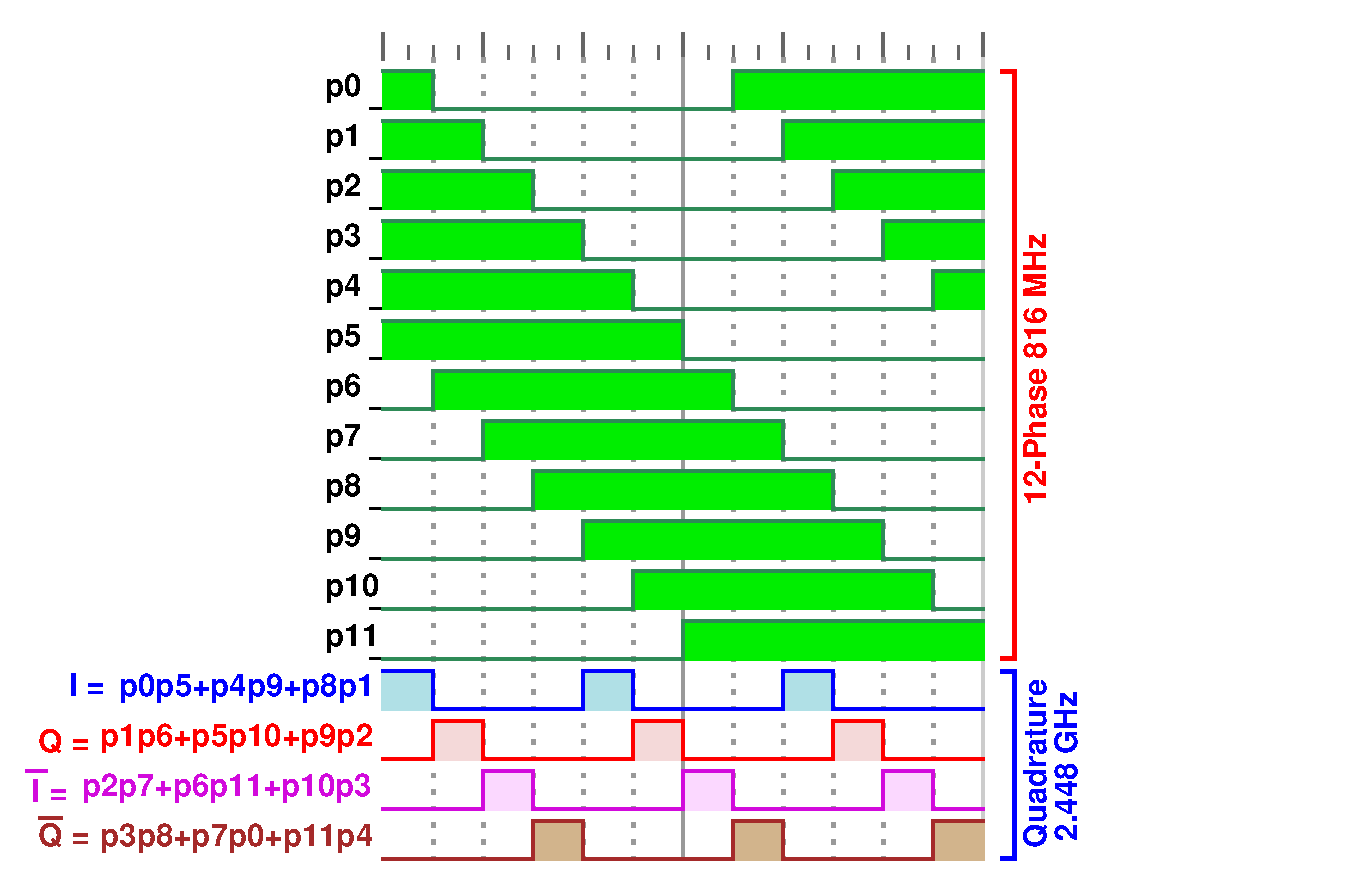
\includegraphics[width=1.0\textwidth, angle=0]{./figs/design/ro_12ph_quad}
			    \caption{Third subharmonic to quadrature full rate conversion.}
			    \label{fig:ro_phases}
			\end{figure}

			\begin{figure}[htb!]
			        \centering
			        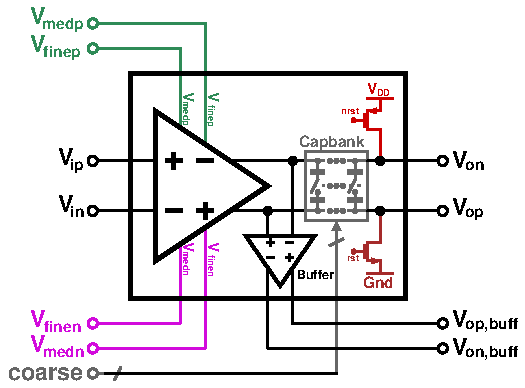
\includegraphics[width=0.5\textwidth, angle=0]{./figs/design/delay_cell_symbol_full}
			    \caption{Ring oscillator delay cell symbol.}
			    \label{fig:delay_cell_symbol}
			\end{figure}

			\begin{figure}[htb!]
			        \centering
			        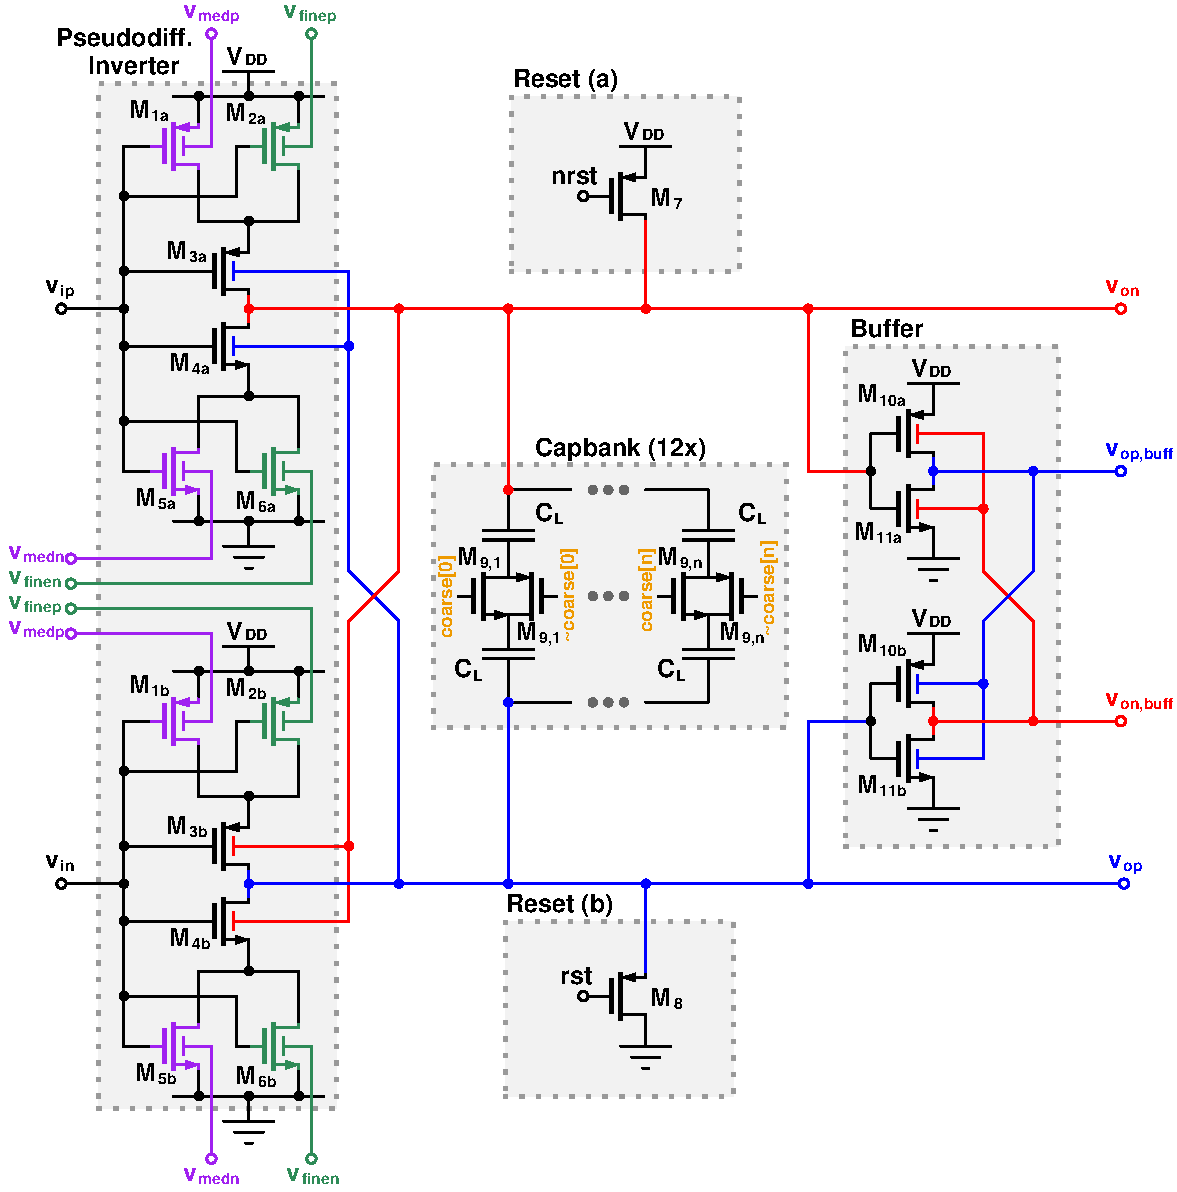
\includegraphics[width=0.8\textwidth, angle=0]{./figs/design/delay_cell_full}
			    \caption{Ring oscillator delay cell full circuit.}
			    \label{fig:delay_cell_circuit}
			\end{figure}
			\begin{figure}[htb!]
			        \centering
			        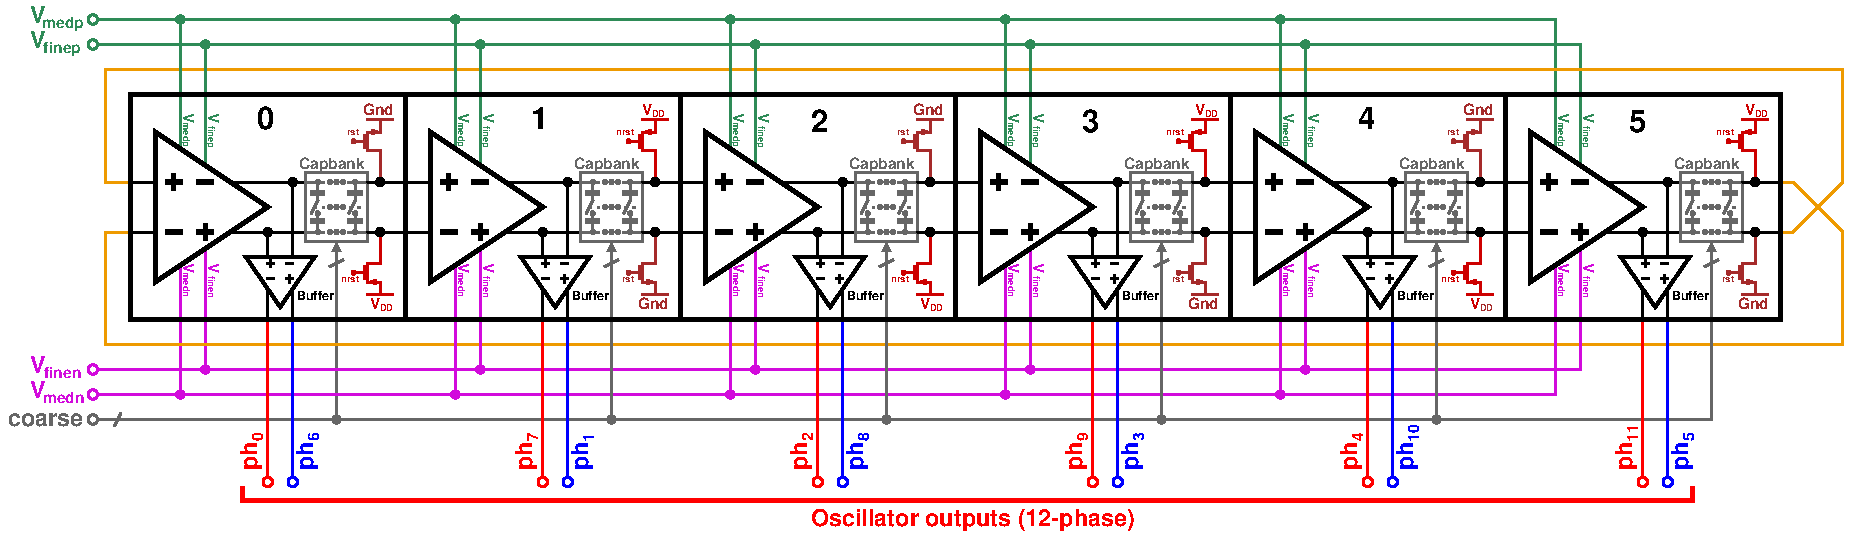
\includegraphics[width=1.5\textwidth, angle=90]{./figs/design/rosc_full_6stg}
			    \caption{Ring oscillator full schematic.}
			    \label{fig:full_6sg_ro}
			\end{figure}


	 Compare RO model (back gate linearity, VDD tuning) to data. There is agreement.
		\subsubsection{Layout}








% ################################################################################################
% ################################################################################################
	\pagebreak\FloatBarrier
	\subsection{Loop Filter}
	For selection of a loop filter, some basic criteria have been selected for desirable synthesizer behavior:
	\begin{enumerate}[itemsep=0pt,label=\protect\mycirc{\arabic*}]
		\setlength\itemsep{-0.8em}
		\item Zero steady state error, for accuracy of the synthesized frequency.
		\item Minimize complexity of implemented logic (i.e. minimize the number of loop filter poles and zeros).
		\item Low pass response of PLL in closed-loop.
	\end{enumerate}
	From this author's previous work \cite{Me}, it was established that the pole-zero filter satisfying these requirements is a proportional-integral controller.

\subsubsection{Proportional-integral Loop Filter}
 A proportional-integral controller \cite{ogata_2010_pid} is given in equation \ref{eq:pi_pll_tf}, containing an proportional gain term $K_p$, and an integral gain term $K_p$. This can be optionally represented using a pole at zero and a zero with $\omega_z = K_i/K_p$:
			\begin{equation} \label{eq:pi_pll_tf}
				\textnormal{H}_{LF}(s) = K_p + \frac{K_i}{s}  = \frac{K_i}{s}\left(\frac{s}{\omega_z} + 1\right) 
			\end{equation}
			Substitution of this controller into the PLL closed loop transfer function (equation \ref{eq:cont_pll_tf2}) results in:
			\begin{equation}\label{eq:pi_bbpdpll_tf}
				T(s) = \frac{\Phi_{out}(s)}{\Phi_{ref}(s)} =  \frac{ 2\pi K_{BBPD}K_{DCO}K_{i} \left(\frac{s}{\omega_z} + 1\right) }{s^2 + 2\pi K_{BBPD}K_{DCO}K_{i}\left(\frac{s}{\omega_z} + 1\right) }
			\end{equation}

	\subsubsection{Discretization of Loop Filter}\label{disc_lf_comp_pi}
		Using the continuous filter discretization approach described in section \ref{lf-discretization} on the loop filter of equation \ref{eq:pi_pll_tf} results in equation \ref{eq:z_lf}. When converting a continuous time PLL model into a discrete time controller implementation, a commonly cited rule of thumb in PLL literature states that the PLL loop bandwidth should be contstrained as $BW_{loop} \leq$  0.1$f_{ref}$ \cite{gardner_1980} (here $\Delta T_s = 1/f_{ref}$). This is due to the fact that low degrees of oversampling lead to deviations between continuous PLL models and real sampled-PLL performance, possibly causing instability or sub-optimal performance versus an intended design.
		\begin{align}
			\textnormal{H}_{LF}(z) & = \left.\frac{K_i}{s}\left(\frac{s}{\omega_z} + 1\right)\right\vert_{s=\frac{1}{\Delta T_s}(1-z^{-1})}
			&= K_p\frac{(1+\omega_z\Delta T_s)-z^{-1}}{1- z^{-2}}\label{eq:z_lf}
		\end{align}

		The transformation of equation \ref{eq:z_lf} into a digitally implementable design as a direct form 1 IIR filter shown in figure \ref{fig:filt_imple}. Its filter coefficients given by equations \ref{eq:b0_coef} and \ref{eq:b1_coef}.
		\begin{figure}[htb!]
			\center\fontfamily{\sfdefault}\selectfont
% XCircuit output "filter_arch_pi.tex" for LaTeX input from filter_arch_pi.ps
\def\putbox#1#2#3#4{\makebox[0.00000in][l]{\makebox[#1][l]{}\raisebox{\baselineskip}[0.00000in][0.00000in]{\raisebox{#2}[0.00000in][0.00000in]{\scalebox{#3}{#4}}}}}
\def\rightbox#1{\makebox[0.00000in][r]{#1}}
\def\centbox#1{\makebox[0.00000in]{#1}}
\def\topbox#1{\raisebox{-0.60\baselineskip}[0.00000in][0.00000in]{#1}}
\def\midbox#1{\raisebox{-0.20\baselineskip}[0.00000in][0.00000in]{#1}}
   \scalebox{1}{
   \normalsize
   \parbox{5.54167in}{
   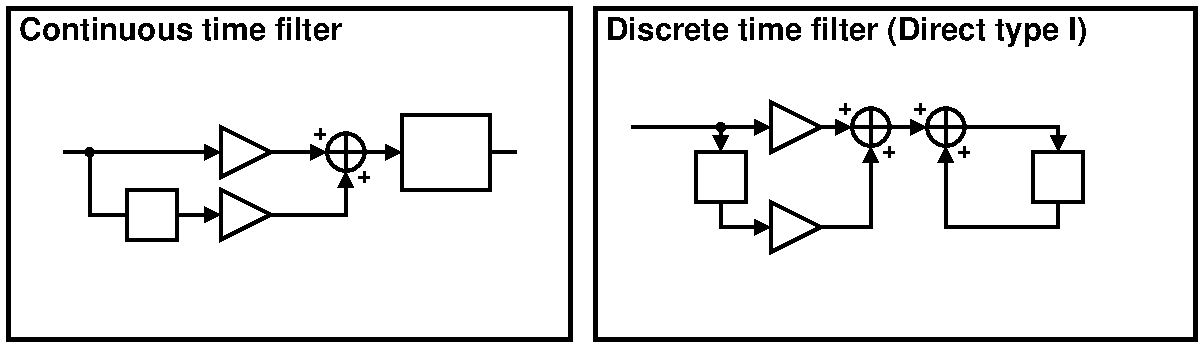
\includegraphics[scale=0.70000]{./figs/filter_arch_pi.pdf}\\
   % translate x=1728 y=944 scale 0.38
   \putbox{1.91800in}{0.90300in}{0.96}{$\frac{1}{\frac{s}{\omega_p} + 1}$}%
   \putbox{1.14800in}{1.01500in}{0.96}{$K_p$}%
   \putbox{1.14800in}{0.72800in}{0.96}{$K_i$}%
   \putbox{0.60900in}{0.58100in}{0.96}{$1/s$}%
   \putbox{0.25900in}{0.98700in}{0.96}{x[n]}%
   \putbox{2.35900in}{0.98700in}{0.96}{y[n]}%
   \putbox{2.92600in}{1.10600in}{0.96}{x[n]}%
   \putbox{4.99800in}{1.01500in}{0.96}{\rotatebox{-360}{y[n]}}%
   \putbox{3.26200in}{0.75600in}{0.96}{$z^{-1}$}%
   \putbox{3.73100in}{1.13400in}{0.96}{b$_0$}%
   \putbox{3.73100in}{0.66500in}{0.96}{b$_1$}%
   \putbox{4.83700in}{0.75600in}{0.96}{$z^{-1}$}%
   \putbox{4.99800in}{0.55300in}{0.96}{y[n-1]}%
   } % close 'parbox'
   } % close 'scalebox'
   \vspace{-\baselineskip} % this is not necessary, but looks better
\fontfamily{\rmdefault}\selectfont

			\caption{Implementation of filter.}
			\label{fig:filt_imple}
		\end{figure}

		\begin{align}
			b_0 &= K_p (1+\omega_z\Delta T_s) \label{eq:b0_coef}\\
			 b_1 &= -K_p \label{eq:b1_coef}
		\end{align}

\subsubsection{Optimal Filter Selection (Noisy BBPD)}
			Optimization of a loop filter under BBPD operation will be performed by minimizing the total integrated phase noise power out of the PLL. First, some mathematical simplifications of the PLL model are introduced. Rewriting equation \ref{eq:pi_bbpdpll_tf} with substitutions $\omega_z = K_i/K_p$ and $\mathrm{K} = 2\pi K_{BBPD}K_{DCO}K_{i}$:
			\begin{equation} \label{eq:simp_pi_pll_tf}
				T(s) = \frac{\Phi_{out}(s)}{\Phi_{ref}(s)} = \frac{s\frac{K}{\omega_z} + K }{s^2 + s\frac{K}{\omega_z} + K}
			\end{equation}
			The denominator can be redefined in terms of a natural frequency $\omega_n$ and damping ratio $\zeta$:
			\begin{equation}
				s^2 + s\frac{K}{\omega_z} + K = s^2 + s2\zeta\omega_n + \omega_n^2
			\end{equation}
			Thus, $\omega_n = \sqrt{K}$, and $\omega_z = \sqrt{K}/2\zeta$. The poles of equation \ref{eq:simp_pi_pll_tf} are then located at s = $\zeta\sqrt{K} \pm j\sqrt{K}\sqrt{1-\zeta^2}$. The time constant of the PLL is obtained from the real portion of the dominant pole in equation \ref{eq:simp_pi_pll_tf}:
			\begin{equation}
				\tau = \frac{1}{|\min(\Re(\{s_{p1}, s_{p2}\}))|}
			\end{equation}
			 It is of interest to minimize settling time of the PLL (i.e. time constant), thus maximizing the frequency of the dominant pole of the PLL is of interest. In the pole-zero plot of figure \ref{fig:pi_pll_pz}, the dominant pole of equation \ref{eq:simp_pi_pll_tf} is observed to be maximized with $\zeta=1$ (loci are oriented based on increasing $\zeta$ values). Citing Razavi \cite{razavi_2017}, $\zeta$ is typically 
			"chosen to be $>\sqrt{2}/2$ or even 1 to avoid excessive ringing." According it has been chosen to fix $\zeta=1$ for the PI-controller. 
			\begin{figure}[htb!]
				\center\fontfamily{\sfdefault}\selectfont
% XCircuit output "pi_pz_plot.tex" for LaTeX input from pi_pz_plot.ps
\def\putbox#1#2#3#4{\makebox[0.00000in][l]{\makebox[#1][l]{}\raisebox{\baselineskip}[0.00000in][0.00000in]{\raisebox{#2}[0.00000in][0.00000in]{\scalebox{#3}{#4}}}}}
\def\rightbox#1{\makebox[0.00000in][r]{#1}}
\def\centbox#1{\makebox[0.00000in]{#1}}
\def\topbox#1{\raisebox{-0.60\baselineskip}[0.00000in][0.00000in]{#1}}
\def\midbox#1{\raisebox{-0.20\baselineskip}[0.00000in][0.00000in]{#1}}
   \scalebox{1}{
   \normalsize
   \parbox{4.20000in}{
   \includegraphics[scale=0.70000]{./figs/pi_pz_plot.pdf}\\
   % translate x=800 y=416 scale 0.38
   \putbox{2.85600in}{0.67900in}{1.20}{$\Re(s)$}%
   \putbox{2.30300in}{1.52600in}{1.20}{$\Im(s)$}%
   \putbox{1.89000in}{0.21700in}{1.20}{$\sqrt{\mathrm{K}}$}%
   \putbox{1.45600in}{1.36500in}{1.20}{$\zeta\sqrt{\mathrm{K}}$}%
   \putbox{2.38700in}{0.95900in}{1.20}{$\sqrt{\mathrm{K}}/2\zeta$}%
   } % close 'parbox'
   } % close 'scalebox'
   \vspace{-\baselineskip} % this is not necessary, but looks better
\fontfamily{\rmdefault}\selectfont

				\caption{PI-controller PLL pole-zero locations.}
				\label{fig:pi_pll_pz}
			\end{figure}
			\FloatBarrier
			% To illustrate the effect of the damping ratio $\zeta$, figure \ref{fig:pi_pll_response} illustratesexample frequency and step responses of a PI-controlled PLL. It is observed that increasing ringing and peaking is obtained with increasing values of $\zeta$. This is undesirable from a stability standpoint, and increased peaking in the PLL transfer function will increase output phase noise contributions, also undesirable. Therefore, the selection of $\zeta=1$ is solidified.
			% \begin{figure}[htb!]
			% 	\center\includegraphics[width=1.0\textwidth, angle=0]{figs/pi_pll_response.pdf}
			% 	\caption{Example PI-PLL responses with varied $\zeta$.}
			% 	\label{fig:pi_pll_response}
			% \end{figure}
			% \FloatBarrier
			With $\zeta$ is constrained to 1, the final simplified PLL closed loop transfer function is in equation \ref{eq:simp_pi_pll_tf_z1}. The form of this equation is favorable for integration, due to the selection of $\zeta$=1.
			\begin{equation} \label{eq:simp_pi_pll_tf_z1}
				T(s) = \frac{2\sqrt{K}s + K }{s^2 + 2\sqrt{K}s + K}
			\end{equation}
			
			Now, the PLL output referred noise power of the oscillator and BBPD may be calculated. First, if the PLL-less oscillator is defined as equation \ref{eq:osc_spectrum}, where $S_{0_{osc}}$ is defined as the oscillator spectral density at 1 Hz frequency offset from the carrier. This takes the form of the theoretical limit for ring oscillator phase noise in section \ref{sec:ro_pn_limit}, with the minimum limit for $S_{0_{osc}}$ given in \ref{eq:min_norm_osc_psd}. For the purposes of this work, T = 300K, $f_{osc}$ = 2.448 GHz, $P_{DC}$ = 80$\mu$W, resulting in a minimum value of $S_{0_{osc},min}$ = 2274 rad$^2$/Hz. 
			\begin{equation}\label{eq:osc_spectrum} 
				\mathcal{L}(f) = \frac{S_{0_{osc}}}{f^2} 
			\end{equation} 
			\begin{equation}\label{eq:min_norm_osc_psd} 
				S_{0_{osc},min} = \left.\mathcal{L}_{min}(f)f^2\right|_{f=1} = \frac{7.33 k_B T f_{osc}^2}{P_{DC}} \hspace{1em}\textnormal{rad}^2/\textnormal{Hz}
			\end{equation}
			The PLL output spectum is then computed as: 
			\begin{align}\label{eq:out_psd_dco_pll3} 
				S_{\Phi n_{DCO,out}}(f) &= \mathcal{L}(f)|1-\textnormal{T}(f)|^2  =  \frac{S_{0_{osc}}}{f^2}|1-\textnormal{T}(f)|^2  
			\end{align} Now, $|1-\textnormal{T}(f)|^2$ is found to be after much simplification:
			\begin{equation} |1-\textnormal{T}(f)|^2 =
				\frac{f^4}{\left(f^2+\frac{K}{(2\pi)^2}\right)^2} 
			\end{equation} 

			Thus, re-evaluating equation \ref{eq:out_psd_dco_pll3} yields:
			\begin{align}\label{eq:out_psd_dco_pll4} 
				S_{\Phi n_{DCO,out}}(f) &= S_{0_{osc}}\frac{f^2}{\left(f^2+\frac{K}{(2\pi)^2}\right)^2} 
			\end{align} 

			The total PLL phase noise power associated with the oscillator, $\sigma_{\Phi_{n,DCO}}^2$ is achieved by integrating equation \ref{eq:out_psd_dco_pll4} with respect to frequency.
			\begin{align}\label{eq:out_psd_dco_pll5} \sigma_{\Phi_{n,DCO}}^2 =
				\int_{-\infty}^{\infty} S_{\Phi n_{DCO,out}}(f)df &=
				S_{0_{osc}}\int_{-\infty}^{\infty}\frac{f^2}{\left(f^2+\frac{K}{(2\pi)^2}\right)^2}df
				\\ &= S_{0_{osc}}\frac{\pi^2}{\sqrt{K}} 
			\end{align} 

			Next, the total BBPD noise at the PLL output is computed. The expression for BBPD noise density in equation \ref{eq:out_psd_bbpd_pll3} will be used, and for which $|\textnormal{T}(f)|^2$ must be computed. This is: 
			\begin{equation} 
				|\textnormal{T}(f)|^2 =
				\frac{4\frac{K}{(2\pi)^2}f^2 +
				\frac{K^2}{(2\pi)^4}}{\left(f^2+\frac{K}{(2\pi)^2}\right)^2} 
			\end{equation}

			The resulting BBPD spectral density equation is:
			\begin{align}\label{eq:out_psd_bbpd_pll4} 
				S_{\Phi n_{BBPD,out}}(f) & =
				\frac{\frac{\pi}{2}(\sigma^2_{\phi_j} +
				\sigma^2_{\phi_n})-\sigma^2_{\phi_n}}{f_{ref}}\left|\mathrm{T}(f)\right|^2
				\\&= \frac{\frac{\pi}{2}(\sigma^2_{\phi_j} +
				\sigma^2_{\phi_n})-\sigma^2_{\phi_n}}{f_{ref}}\cdot\frac{4\frac{K}{(2\pi)^2}f^2
				+ \frac{K^2}{(2\pi)^4}}{\left(f^2+\frac{K}{(2\pi)^2}\right)^2} 
			\end{align} 

			The total PLL phase noise power associated with the BBPD, $\sigma_{\Phi_{n,BBPD}}^2$ is achieved by integrating equation \ref{eq:out_psd_bbpd_pll4} with respect to frequency:
			\begin{align}\label{eq:out_psd_bbpd_pll5} 
				\sigma_{\Phi_{n,BBPD}}^2 & =
				\frac{\frac{\pi}{2}(\sigma^2_{\phi_j} +
				\sigma^2_{\phi_n})-\sigma^2_{\phi_n}}{f_{ref}}\int_{-\infty}^{\infty}\frac{4\frac{K}{(2\pi)^2}f^2
				+ \frac{K^2}{(2\pi)^4}}{\left(f^2+\frac{K}{(2\pi)^2}\right)^2}df\\ &= 
				\frac{5\sqrt{K}}{4f_{ref}}\cdot\left[\frac{\pi}{2}(\sigma^2_{\phi_j} +
			\sigma^2_{\phi_n})-\sigma^2_{\phi_n}\right] \end{align} 

			The total noise out of the PLL is therefore the sum of $\sigma_{\Phi_{n,BBPD}}^2$ and $\sigma_{\Phi_{n,DCO}}^2$ : 
			\begin{align} \label{eq:total_pll_pn_pow}
				\sigma^2_{\phi_n}  = \sigma_{\Phi_{n,DCO}}^2 + \sigma_{\Phi_{n,BBPD}}^2 =
				S_{0_{osc}}\frac{\pi^2}{\sqrt{K}} +
				\frac{5\sqrt{K}}{4f_{ref}}\cdot\left[\frac{\pi}{2}(\sigma^2_{\phi_j} +
				\sigma^2_{\phi_n})-\sigma^2_{\phi_n}\right] 
			\end{align} 
			Reorganization of equation \ref{eq:total_pll_pn_pow} in terms of $\sigma^2_{\phi_n}$ yields:
			\begin{align} \label{eq:total_pll_pn_pow2} \sigma^2_{\phi_n}  =
				\frac{S_{0_{osc}}\frac{\pi^2}{\sqrt{K}} +
				\frac{5\pi\sqrt{K}}{8f_{ref}}\sigma^2_{\phi_j}}{1-\frac{5\sqrt{K}}{4f_{ref}}(\frac{\pi}{2}-1)}
			\end{align}			 

			In the special case of an ideal BBPD where $\sigma^2_{\phi_j}$ = 0, the optimal value of $K$ that minimizes total phase noise can be determined by solving for $d\sigma^2_{\phi_n}/dK = 0$, yielding:
			\begin{align} \label{eq:k_opt} K_{opt} =
				\left(\frac{4}{5}\cdot\frac{f_{ref}}{\pi-2}\right)^2 
			\end{align}	 

			The corresponding optimal value of $\sigma^2_{\phi_n} $ is in equation \ref{eq:total_pll_pn_pow_opt}. This should be the absolute best case achievable with a BBPD PLL with a PI-controller. For this design, with 80$\mu$W oscillator power at 2.448 GHz, 16 MHz reference, and 300K ambient temperature, the theoretical best attainable phase noise is $\sigma^2_{\phi_{n,opt}}=0.004$, or a CNR of 24 dB, above the desired 20 dB. Therefore, the current design targets are feasible under ideal circumstances. 
			\begin{align} \label{eq:total_pll_pn_pow_opt} 
				\sigma^2_{\phi_{n,opt}}  =
				\frac{5\pi^2S_{0_{osc}}}{f_{ref}}\left(\frac{\pi}{2}-1\right) 
			\end{align}	 

			In the presence of a non-ideal phase detector having phase noise power $\sigma^2_{\phi_j} = (2\pi f_{osc})^2\sigma^2_{t_j}$, the optimal value K that minimizes phase noise is obtained as the root of $d\sigma^2_{\phi_n}/dK = 0$ in equation \ref{eq:noisy_opt_k}. The obtained result for $K_{opt}$ may be substitued into equation \ref{eq:total_pll_pn_pow2} to determine the total noise power $\sigma^2_{\phi_n}$. 
			\begin{equation}\label{eq:noisy_opt_k}
				K_{opt} = \left[\frac{S_{0_{osc}}\pi(\pi-2)}{\sigma^2_{\phi_j}} -
				\sqrt{\frac{S_{0_{osc}}^2\pi^2(\pi-2)^2}{\sigma^4_{\phi_j}} +
				\frac{S_{0_{osc}}8\pi f_{ref}}{5\sigma^2_{\phi_j}}} \right]^2 
			\end{equation}

			The parameter of K has a direct relationship to the closed loop bandwidth $BW_{loop}$ of the PLL, which is determined by solving $|T(f)|^2 = 0.5$. The result is given in equation \ref{eq:loop_bw}. 
			\begin{equation}\label{eq:loop_bw} 
				BW_{loop} = \frac{1}{2\pi}\sqrt{K}\sqrt{3+
				\sqrt{10}} 
			\end{equation} 

			As mentioned before, it is advisable to observe a limit of loop bandwidth of at most $BW_{loop}$ = 0.1$f_{ref}$. The coefficient $\alpha$ is defined here now to describe the loop bandwidth-reference frequency ratio, where $BW_{loop} = \alpha f_{ref}$. Interestingly, solving the system of equations given by equation \ref{eq:k_opt} and equation \ref{eq:loop_bw} provides an ideal ratio of $BW_{loop}$ and $f_{ref}$, being $\alpha$=0.28, which exceeds the rule of thumb $\alpha$=0.1. Thus, in the case that $\alpha$ must be constrained for sampling reasons, equation \ref{eq:k_alpha} is found to determine K. Thus with a 16 MHz reference, and $\alpha$=0.1, $K=1.64\times10^{13}$. 
			\begin{equation}\label{eq:k_alpha} 
				K_\alpha = \frac{(2\pi\alpha f_{ref})^2}{3
				+ \sqrt{10}} 
			\end{equation}

			It is best to be as near to the optimal value of $\alpha$ as possible. Figure \ref{fig:alpha_v_pn} demonstrates the effect of $\alpha$ on the phase noise power (normalized to the optimal value). It is seen that the total phase noise asymptotically grows to infinity as $\alpha$ approaches 0 and 0.55. In the case of $\alpha$ = 0.1, the phase noise is expected to be 1.69 times the optimal value, resulting in a 2.3 dB degredation from optimal, implying that the best case CNR is 21.7 dB with 80$\mu$W oscillator power at 2.448 GHz, 16 MHz reference, and 300K ambient temperature.

			\begin{figure}[htb!]
				\center\includegraphics[width=0.6\textwidth, angle=0]{./figs/design/alpha_v_pn}
				\caption{Phase noise power (normalized) versus $\alpha$.}
				\label{fig:alpha_v_pn}
			\end{figure}

			It is possible to derive a constraint for BBPD jitter $\sigma^2_{\phi_j}$ in terms of $\alpha$ and a target $\sigma^2_{\phi_n}$ (i.e. CNR value), which allows for the performance specification for the physical BBPD to be set. Equation \ref{eq:bbpd_jit_pn} defines the maximum allowable phase noise power due to BBPD jitter, and equation \ref{eq:bbpd_t_jit_rms} defines the maximum RMS timing jitter of the same detector. In the case of 2.448 GHz operation, with 20 dB of CNR, and $\alpha$ = 0.1, the maximum allowable RMS BBPD jitter is $\sigma_{t_j}$ = 4.75 ps.
			\begin{equation}\label{eq:bbpd_jit_pn}
				\sigma^2_{\phi_j} \leq \sigma^2_{\phi_n}\left[\frac{4\sqrt{3+\sqrt{10}}}{5\pi^2\alpha} +\frac{2}{\pi} - 1 \right] - \frac{2S_{0_{osc}}(3 + \sqrt{10})}{5\pi\alpha^2f_{ref}}
			\end{equation}
			\begin{equation}\label{eq:bbpd_t_jit_rms}
				\sigma_{t_j} \leq \frac{1}{2\pi f_{osc}}\sqrt{\sigma^2_{\phi_n}\left[\frac{4\sqrt{3+\sqrt{10}}}{5\pi^2\alpha} +\frac{2}{\pi} - 1 \right] - \frac{2S_{0_{osc}}(3 + \sqrt{10})}{5\pi\alpha^2f_{ref}}}
			\end{equation}

			Now with theory in place to optimize PLL performance, mapping of the optimal parameter $K$ onto the loop filter of equation \ref{eq:pi_pll_tf} will be considered. Recall that $\omega_z = K_i/K_p = \sqrt{K}/2\zeta$ and $K = 2\pi K_{BBPD}K_{DCO}K_{i}$. The parameters $K_i$, $K_p$, and $\omega_z$ are thus provided in equations \ref{eq:wz_}-\ref{eq:ki_}.
			\begin{align}
				\omega_z &= \frac{\sqrt{K}}{2}\label{eq:wz_}\\
				K_p &= \frac{\sqrt{K}}{\pi K_{BBPD}K_{DCO}} = \frac{\sqrt{K}\sqrt{\sigma^2_{\phi_j} + \sigma^2_{\phi_n}}}{\sqrt{2\pi}K_{DCO}}\\
				K_i &= \frac{K}{2\pi K_{BBPD}K_{DCO}} = \frac{K\sqrt{\sigma^2_{\phi_j} + \sigma^2_{\phi_n}}}{2\sqrt{2\pi}K_{DCO}}\label{eq:ki_}
			\end{align}
			Converting the filter design into discrete time equivalent results in equations \ref{eq:b0} and \ref{eq:b1}
			\begin{align}
				b_0 &= \frac{\sqrt{K}\sqrt{\sigma^2_{\phi_j} + \sigma^2_{\phi_n}}}{\sqrt{2\pi}K_{DCO}}\left(1+\frac{\sqrt{K}}{2f_{ref}}\right)\label{eq:b0}\\
				 b_1 &=  - \frac{\sqrt{K}\sqrt{\sigma^2_{\phi_j} + \sigma^2_{\phi_n}}}{\sqrt{2\pi}K_{DCO}}\label{eq:b1}
			\end{align}
			If design of the PLL is with fixed target for $\sigma^2_{\phi_n}$ (CNR), has a known $\sigma^2_{\phi_j}$ for the BBPD, and $\alpha$ is selected to be constant (i.e. 0.1), the filter coefficients may be calculated as in equations \ref{eq:b0_} and \ref{eq:b1_}.

			\begin{align}
				b_0 &= \frac{\alpha f_{ref}\sqrt{2\pi}\sqrt{\sigma^2_{\phi_j} + \sigma^2_{\phi_n}}}{\sqrt{3+\sqrt{10}}K_{DCO}} \left(1+\frac{\pi\alpha}{\sqrt{3+\sqrt{10}}}\right)\label{eq:b0_}\\
				 b_1 &= - \frac{\alpha f_{ref}\sqrt{2\pi}\sqrt{\sigma^2_{\phi_j} + \sigma^2_{\phi_n}}}{\sqrt{3+\sqrt{10}}K_{DCO}}\label{eq:b1_}
			\end{align}
	

%%%%%%%%%%%%%%%%%%%%%%%%%%%%%%%%%%%%%%%%%%%%%%%%%%%

			\FloatBarrier\subsubsection{Emergent Bang-Bang PLL Phase Noise}\label{sec:bb_noise}
			Since the output of BBPD is quantized to $\pm$ 1, the use of a PI loop filter architecture results in only 4 possible values that node {\color{blue}\textbf{x}} can be valued as shown in the simplified BBPD-PLL model of figure \ref{fig:simp_bbpdpll}. These are $\lfloor b_0+b_1 \rfloor$, $\lfloor b_0-b_1 \rfloor$, $\lfloor -b_0+b_1 \rfloor$, $\lfloor -b_0-b_1 \rfloor$. The result of this is the loop filter output {\color{teal}\textbf{u}} must increment by one of these four values every reference cycle. 

		\begin{figure}
			\center\includegraphics[width=0.8\textwidth, angle=0]{./figs/design/simplified_bbpll}
			\caption{Simplified model of BBPD-PLL}
			\label{fig:simp_bbpdpll}
		\end{figure}
		The worst case scenario of this is the BBPD outputting an alternating sequence of +1/-1/+1/-1... , for which the output will toggle between $\lfloor b_0-b_1 \rfloor$ and $\lfloor -b_0+b_1 \rfloor$. In terms of frequency, the output will shift up and down by $K_{DCO}\lfloor b_0-b_1 \rfloor$ and $\lfloor -b_0+b_1 \rfloor$ every other cycle, which can be substantial depending on the product of those factors. In the phase domain, this results in a cyclostationary triangle-wave like phase trajectory (ignoring other sources of phase noise), as shown in figure \ref{fig:cylostationary}. The worst case increment in phase per cycle is given in equation \ref{eq:cyclo_dph}. In the frequency domain, this cyclostationary behavior can result in spurs, as shown in figure \ref{fig:cylostationary_spurs}. When phase noise from other processes in the PLL are large enough that the they dwarf the worst case cyclostationary behavior, it is expected that output of the BBPD will be stochastically scrambled and the cyclostationary effects will be subsided. 

		\begin{equation}\label{eq:cyclo_dph}
			\Delta \Phi = \frac{2\pi|b_0-b_1|K_{DCO}}{f_{ref}}
		\end{equation}

	\begin{figure}[htb!]
	    \centering
	    \begin{subfigure}{0.5\textwidth}
	        \centering
	        \includegraphics[width=0.8\textwidth, angle=0]{./figs/bbpd_resolution_phase_walk}
	        \caption{ }
	        \label{fig:cylostationary}
	    \end{subfigure}%
	    \begin{subfigure}{0.5\textwidth}
	        \centering
	        \center\includegraphics[width=0.8\textwidth, angle=0]{./figs/spurs_dco}
	        \caption{ }
	        \label{fig:cylostationary_spurs}
	    \end{subfigure}
	    \caption{\textbf{(a)} Worst case cyclostationary behavior of BBPD-PLL, \textbf{(b)} Resulting in spurs from worst case cyclostationary behavior.}
	    \label{fig:cyclostationary_nonsense}
	\end{figure}


	Even if cyclostationary effects are avoided, the quantization of the loop filter output to increments of the four aforementioned values results in an additive phase noise contribution to the PLL. The estimated that the RMS contribution of phase noise to the PLL output due to the quantized steps in frequency from bang-bang operation $\sigma_{\Phi_{BB}}$ is given in equation \ref{eq:bb_jitter}. If this component approaches the magnitude of the other phase noise components, the model assumptions for the BBPD theory derived in this work may be invalid, so prudent selection of parameters should be made to reduce $\sigma_{\Phi_{n_{BB}}}$.

		\begin{equation}\label{eq:bb_jitter}
			\sigma_{\Phi_{n_{BB}}} \approx \frac{\pi|b_0-b_1|K_{DCO}}{f_{ref}}
		\end{equation}
	If $\alpha$ is used to described to loop bandwidth ratio-reference frequency ratio, the quantity $|b_0-b_1|$ is provided in equation \ref{eq:b1_b0}. In the case where $\alpha$ is small (circa 0.1 as followed in this work), $|b_0-b_1| \approx |2b_1|$, so $\sigma_{\Phi_{n_{BB}}}$ may be approximated as in equation \ref{eq:bb_jitter2}
	\begin{equation}\label{eq:b1_b0}
			|b_0-b_1| = \left(2 + \frac{\pi \alpha}{\sqrt{3+\sqrt{10}}}\right)|b_1|
	\end{equation}
	\begin{equation}\label{eq:bb_jitter2}
		\sigma_{\Phi_{n_{BB}}} \approx \frac{2\pi b_1K_{DCO}}{f_{ref}}
	\end{equation}	
	If the dominant noise sources are assumed to be $\sigma^2_{\Phi_{n_{BB}}}$ and oscillator noise, the total phase noise $\sigma^2_{\Phi_{n}}$ equals that in equation \ref{eq:bb_osc_noise}.
	\begin{equation}\label{eq:bb_osc_noise}
		\sigma_{\Phi_{n}}^2 = \sigma_{\Phi_{n,DCO}}^2 + \sigma^2_{\Phi_{n_{BB}}} = S_{0_{osc}}\frac{\pi^2}{\sqrt{K}} + \left( \frac{2\pi b_1K_{DCO}}{f_{ref}} \right)^2
	\end{equation}
	Redefining equation \ref{eq:b1} using $\sigma^2_{\Phi_{n_{BB}}}$ and oscillator noise as the phase noise sources results in equation \ref{eq:b1__}.
		\begin{align}
			 b_1 &=  - \frac{\sqrt{K}\sqrt{\sigma_{\Phi_{n,DCO}}^2 + \sigma^2_{\Phi_{n_{BB}}} }}{\sqrt{2\pi}K_{DCO}} = - \frac{\sqrt{K}\sqrt{  S_{0_{osc}}\frac{\pi^2}{\sqrt{K}} + \left( \frac{2\pi b_1K_{DCO}}{f_{ref}} \right)^2 }}{\sqrt{2\pi}K_{DCO}}\label{eq:b1__} 
		\end{align}
	A resulting expression for $\sigma^2_{\Phi_{n_{BB}}}$ is obtained by solving the system of equations given by \ref{eq:bb_jitter2} and \ref{eq:b1__}.
	 	\begin{equation}
	 		\sigma^2_{\Phi_{n_{BB}}} = \frac{2\pi^3\sqrt{K}S_{0_{osc}}}{f_{ref}^2  - 2\pi K} = \frac{4\pi^4\alpha S_{0_{osc}}}{f_{ref}\sqrt{3+\sqrt{10}}}\cdot \frac{1}{1-\frac{8\pi^3\alpha^2}{\sqrt{3+\sqrt{10}}}}
	 	\end{equation}
	This equation grows asymptotically to infinity with $K=f_{ref}^2/2\pi$, equating to $\alpha = \sqrt{3+\sqrt{10}}/(2\pi)^{3/2}$  = 0.158. $\sigma^2_{\Phi_{n_{BB}}}$ approaches zero for increasingly small values of $\alpha$. Rewriting equation \ref{eq:bb_osc_noise} with the new finding for $\sigma^2_{\Phi_{n_{BB}}}$ results in equation \ref{eq:bb_osc_noise2}. Now $\sigma_{\Phi_{n}}^2$ may be minimized for noise by solving $d\sigma_{\Phi_{n}}^2(K)/dK =0$, yielding equation \ref{eq:kopt_bb}. It is also determined that the optimal value of $\alpha$ is in equation \ref{eq:alpha_opt_bb}, and the optimal total phase noise power is in equation \ref{eq:pn_opt_bb}.
	\begin{equation}\label{eq:bb_osc_noise2}
		\sigma_{\Phi_{n}}^2 = \sigma_{\Phi_{n,DCO}}^2 + \sigma^2_{\Phi_{n_{BB}}} = S_{0_{osc}}\frac{\pi^2}{\sqrt{K}} + \frac{2\pi^3\sqrt{K}S_{0_{osc}}}{f_{ref}^2  - 2\pi K}
	\end{equation}
	\begin{equation} \label{eq:kopt_bb}
		K_{opt} = \frac{f_{ref}^2}{6\pi^2}
	\end{equation}
	\begin{equation} \label{eq:alpha_opt_bb}
		\alpha_{opt} = \frac{\sqrt{3+\sqrt{10}}}{2\pi^2\sqrt{6}} = 0.0513
	\end{equation}
	\begin{equation} \label{eq:pn_opt_bb}
		\left.\sigma_{\Phi_{n}}^2 \right|_{K_{opt}} = \frac{3\sqrt{6}\pi^4S_{0_{osc}}}{f_{ref}}\cdot\frac{1}{3\pi - 1}
	\end{equation}
	In the case of this work with a target of 2.448 GHz, 16 MHz reference, and 300K ambient temperature, the theoretical obtainable CNR is 19.2 dB, or $\sigma_{\Phi_{n}}^2$ = 0.012 rad$^2$. The discrete time filter coefficients for this optimization case are provided in equations \ref{eq:b0_bb} and \ref{eq:b1_bb}.
	\begin{align}
		b_0 &= \frac{\sqrt{\pi f_{ref}\sqrt{6}S_{0_{osc}}}}{2K_{DCO}\sqrt{3\pi-1}}\left( 1 + \frac{1}{2\sqrt{6}\pi} \right) \label{eq:b0_bb}\\
		b_1 &= -\frac{\sqrt{\pi f_{ref}\sqrt{6}S_{0_{osc}}}}{2K_{DCO}\sqrt{3\pi-1}}\label{eq:b1_bb}
	\end{align}

	\subsubsection{Choice of Optimization Strategy}
	Depending on the implementation, either the noise contributions from the phase detector or due to the bang-bang behavior may be the second most dominant noise source after the oscillator. The recommended strategy to calculate the optimal filter design using both approaches, and select the one that results in a larger total phase noise value $\sigma_{\Phi_{n}}^2$.

	In this work, 80$\mu$W oscillator power at 2.448 GHz, 16 MHz reference, and 300K ambient temperature, $K_{DCO}$ = 4.2 kHz/LSB, oscillator noise density at 1 Hz of $\mathcal{L}(f)|_{f=1}$ = 11885 rad$^2$/Hz, and a detector jitter of 1.4 ps RMS, leads to a CNR of 17.2 dB when optimizing for oscillator plus BBPD jitter, and a CNR of 12.7 dB when optimizing for oscillator noise plus emergent bang bang phase noise. Selecting the worse valued result as the accurate model for this implementation then implies that this PLL should be optimized for oscillator noise plus emergent bang bang effects. 

%%%%%%%%%%%%%%%%%%%%%%%%%%%%%%%%%%%%%%%%



	\FloatBarrier

		\subsubsection{Filter Design for Synchronous counter}
			As gear-switching is intended to be used in this work, a separate loop filter will be calculated that is optimized for settling time (i.e. lock time) with the synchronous counter phase detector during initial start up. It was determined in the previous section that the poles of the PI-PLL occur at s = $\zeta\sqrt{K} \pm j\sqrt{K}\sqrt{1-\zeta^2}$, as a conjugate pair. Taking the real portion (same for both) provides for the value of the PLL time constant:
			\begin{equation}
				\tau = \frac{1}{|\min(\Re(\{s_{p1}, s_{p2}\}))|} = \frac{1}{\zeta\sqrt{K}}
			\end{equation}
			If $\delta$ is considered that fraction of the initial frequency error during the lock process that may be achieved for lock, then the PLL lock time is given by equation \ref{eq:locktime}. $\delta$ can be also stated in terms of initial frequency error $\Delta f$, and the frequency tolerance from steady state $f_{tol}$ that is considered to be in lock for a given application.
			\begin{equation}\label{eq:locktime}
				t_s = \frac{-\ln(\delta)}{\zeta\sqrt{K}} = \frac{-\ln\left(\frac{f_{tol}}{|\Delta f|}\right)}{\zeta\sqrt{K}}
			\end{equation}
			It is observed that lock time is decreased by increasing the value of both $\zeta$ and $K$. Again, the constraint $\zeta$=1 due to its favorable characteristics. Thus, it is of interest here to maximize the value of $K$. It is seen that in equation \ref{eq:loop_bw} $K\propto BW_{loop}^2$, thus loop bandwidth should be maximized. Again defining a constraint between loop bandwidth and reference frequency of $\alpha = BW_{loop}/f_{ref}$, equation \ref{eq:k_alpha} can be used to determine the optimal selection of $K$ for a given $\alpha$ and $f_{ref}$. Plugging this into equation \ref{eq:locktime} yields equation \ref{eq:locktime2}.
			\begin{equation}\label{eq:locktime2}
				t_s =  \frac{-\sqrt{3+\sqrt{10}}\ln\left(\frac{f_{tol}}{|\Delta f|}\right)}{2\pi\alpha f_{ref}}
			\end{equation}
			Now, these defined filters parameters will be translated into a filter design. Again, the definitions $K=2\pi K_{PD}K_{DCO}K_{i}$ and $\omega_z = K_i/K_p$ are used. A detector gain $K_{PD}$ must be defined first for the synchronous counter. Since the synchronous counter counts cycles, it in effects converts $2\pi$ of phase into an increment of count of 1. Thus the gain is:
			\begin{equation}
				K_{PD} = \frac{1}{2\pi}
			\end{equation}
			The parameters $K_i$, $K_p$ and $\omega_z$ are then solved for, to result in equations \ref{eq:kp_sc} to \ref{eq:b1_sc}.
			\begin{align}
				K_p & = \frac{4\pi\alpha f_{ref}}{\sqrt{3+\sqrt{10}}K_{DCO}}\label{eq:kp_sc}\\
				K_i & = \frac{(2\pi\alpha f_{ref})^2}{(3+\sqrt{10})K_{DCO}}\\
				\omega_z &= \frac{\pi\alpha f_{ref}}{\sqrt{3+\sqrt{10}}}\label{eq:wz_sc}\\
				b0 &= K_p = \frac{4\pi\alpha f_{ref}}{\sqrt{3+\sqrt{10}}K_{DCO}}  \\
				b1 &= \frac{4\pi\alpha f_{ref}}{\sqrt{3+\sqrt{10}}K_{DCO}}\left( 1 + \frac{\pi\alpha}{\sqrt{3+\sqrt{10}}} \right ) \label{eq:b1_sc}\\
			\end{align}

		\subsubsection{PI-controller phase margin}\label{pi_phase_margin}
			The PI-PLL architecture of this work has a phase margin determined by the damping ratio $\zeta$, given by equation \ref{eq:pm_pi_pll}. Figure \ref{fig:phase_margin} shows phase margin versus $0 \geq \zeta \geq 1$ of the PI-controller PLL. It is recommended to use at least 30-60 degrees in phase margin to achieve stability \cite{ogata_2010_stability}. In this work, $\zeta$ = 1 has been used, so a phase margin of 76 degrees is expected, and accordingly stability should be expected.
			\begin{equation}\label{eq:pm_pi_pll}
				\angle \text{L}(\omega_{ug}) = \frac{180}{2\pi}\arctan\left(2\zeta\sqrt{2\zeta^2 + \sqrt{4\zeta^4+1}}\right)\hspace{1em}[\text{degrees}]
			\end{equation}
			\begin{figure}[htb!]
				\center\includegraphics[width=0.5\textwidth, angle=0]{figs/damping_vs_pm.pdf}
				\caption{PI-controller PLL phase margin versus damping ratio.}
				\label{fig:phase_margin}
			\end{figure}



	% \subsubsection{Discretization of Loop Filter}\label{disc_lf_comp_pi}
	% 	Using the continuous filter discretization approach described in section \ref{lf-discretization} on the loop filter of equation \ref{eq:pi_pll_tf} results in equation \ref{eq:z_lf}.
	% 	\begin{align}
	% 		\textnormal{H}_{LF}(z) & = \left.\frac{K_i}{s}\left(\frac{s}{\omega_z} + 1\right)\right\vert_{s=\frac{1}{\Delta T_s}(1-z^{-1})}
	% 		&= K_p\frac{(1+\omega_z\Delta T_s)-z^{-1}}{1- z^{-2}}\label{eq:z_lf}
	% 	\end{align}

	% 	The transformation of equation \ref{eq:z_lf} into a digitally implementable design as a direct form 1 IIR filter shown in figure \ref{fig:filt_imple}. Its filter coefficients given by equations \ref{eq:b0} and \ref{eq:b1}.
	% 	\begin{figure}[htb!]
	% 		\center\fontfamily{\sfdefault}\selectfont
% XCircuit output "filter_arch_pi.tex" for LaTeX input from filter_arch_pi.ps
\def\putbox#1#2#3#4{\makebox[0.00000in][l]{\makebox[#1][l]{}\raisebox{\baselineskip}[0.00000in][0.00000in]{\raisebox{#2}[0.00000in][0.00000in]{\scalebox{#3}{#4}}}}}
\def\rightbox#1{\makebox[0.00000in][r]{#1}}
\def\centbox#1{\makebox[0.00000in]{#1}}
\def\topbox#1{\raisebox{-0.60\baselineskip}[0.00000in][0.00000in]{#1}}
\def\midbox#1{\raisebox{-0.20\baselineskip}[0.00000in][0.00000in]{#1}}
   \scalebox{1}{
   \normalsize
   \parbox{5.54167in}{
   \includegraphics[scale=0.70000]{./figs/filter_arch_pi.pdf}\\
   % translate x=1728 y=944 scale 0.38
   \putbox{1.91800in}{0.90300in}{0.96}{$\frac{1}{\frac{s}{\omega_p} + 1}$}%
   \putbox{1.14800in}{1.01500in}{0.96}{$K_p$}%
   \putbox{1.14800in}{0.72800in}{0.96}{$K_i$}%
   \putbox{0.60900in}{0.58100in}{0.96}{$1/s$}%
   \putbox{0.25900in}{0.98700in}{0.96}{x[n]}%
   \putbox{2.35900in}{0.98700in}{0.96}{y[n]}%
   \putbox{2.92600in}{1.10600in}{0.96}{x[n]}%
   \putbox{4.99800in}{1.01500in}{0.96}{\rotatebox{-360}{y[n]}}%
   \putbox{3.26200in}{0.75600in}{0.96}{$z^{-1}$}%
   \putbox{3.73100in}{1.13400in}{0.96}{b$_0$}%
   \putbox{3.73100in}{0.66500in}{0.96}{b$_1$}%
   \putbox{4.83700in}{0.75600in}{0.96}{$z^{-1}$}%
   \putbox{4.99800in}{0.55300in}{0.96}{y[n-1]}%
   } % close 'parbox'
   } % close 'scalebox'
   \vspace{-\baselineskip} % this is not necessary, but looks better
\fontfamily{\rmdefault}\selectfont

	% 		\caption{Implementation of filter.}
	% 		\label{fig:filt_imple}
	% 	\end{figure}

	% 	\begin{align}
	% 		b_0 &= K_p (1+\omega_z\Delta T_s)\\
	% 		 b_1 &= -K_p 
	% 	\end{align}
	% 	In the case of a BBPD PLL:
	% 	\begin{align}
	% 		b_0 &= \frac{\sqrt{K}\sqrt{\sigma^2_{\phi_j} + \sigma^2_{\phi_n}}}{\sqrt{2\pi}K_{DCO}}\left(1+\frac{\sqrt{K}}{2f_{ref}}\right)\label{eq:b0}\\
	% 		 b_1 &=  - \frac{\sqrt{K}\sqrt{\sigma^2_{\phi_j} + \sigma^2_{\phi_n}}}{\sqrt{2\pi}K_{DCO}}\label{eq:b1}
	% 	\end{align}
	% 	If design of the PLL is with fixed target for $\sigma^2_{\phi_n}$ (CNR), has a known $\sigma^2_{\phi_j}$ for the BBPD, and $\alpha$ is selected to be constant (i.e. 0.1), the filter coefficients may be calculated as in equations \ref{eq:b0_} and \ref{eq:b1_}.

	% 	\begin{align}
	% 		b_0 &= \frac{\alpha f_{ref}\sqrt{2\pi}\sqrt{\sigma^2_{\phi_j} + \sigma^2_{\phi_n}}}{\sqrt{3+\sqrt{10}}K_{DCO}} \left(1+\frac{\pi\alpha}{\sqrt{3+\sqrt{10}}}\right)\label{eq:b0_}\\
	% 		 b_1 &= - \frac{\alpha f_{ref}\sqrt{2\pi}\sqrt{\sigma^2_{\phi_j} + \sigma^2_{\phi_n}}}{\sqrt{3+\sqrt{10}}K_{DCO}}\label{eq:b1_}
	% 	\end{align}
	% 	%%%%


%%%%%%%%%%%%%%%%%%%%%%%%%%%%%%%%%%%%%%%%




		\subsubsection{Implementation}
			The filter has been chosen to be implemented with separate parts to implement the feedforward parts for each phase detector of the PI-controller, but with a common integrator at the output, as shown in figure \ref{fig:pi_dig_imp}. This approach to reduce power in steady state operation (using the BBPD). The rationale is that the synchronous counter is a linear detector, thus requires multipliers in the datapath to implement the filter, whereas the BBPD only outputs two values (+1 and -1), so the multipliers can be replaced with multiplexers that select between two sets of possible products ($\pm b_0$ and $\pm b_1$) depending on the input. It is lower energy to operate a multiplexer than an array multiplier due to substantially lower complexity of logic, so the usage of two multiplexers in steady to implement the multipliers will result in substantial power savings. The usage of a common integrator used in both detector modes allows for seamless continuity of output value during transition between detector modes. 

			The computed filter coefficients $\{b_0$, $b_1\}$ for the PLL must be digitized into finite length signed two's complement words. A two's complement data word contains one sign bit, and variable number of bits representing the integer and fractional portions of the encoded number. The author of this work has previously devised a method \cite{Me} for automatically computing the number of bits required to represent a filter in PLL. First, the selection of number of integer bits \texttt{int\_bits} is determined by considering the integer part of the discrete filter coefficients. If the integer portions of the filter coefficients $\{b_0$, $b_1\}$ are divided into positive and negative valued sets \texttt{pos\_ints} and \texttt{neg\_ints}, is therefore given in equation \ref{eq:int_bits}. Computation of the fractional portion is more complicated, and is based on reducing the quantization noise floor of the loop filter below other noise components of the PLL. The PLL design framework from \cite{Me} will be used in this work for determining the minimum digitized representation size of filter coefficients.
			\begin{align}
				\mathtt{pos\_int\_bits} &= \left\lfloor \log_2\left(\max\left(\left\lfloor \mathtt{pos\_ints} \right\rfloor\right)\right) \right\rfloor +1\\
				\mathtt{neg\_int\_bits} &= \left\lceil \log_2\left(\max\left(\left\lfloor \mathtt{neg\_ints} \right\rfloor\right)\right) \right\rceil\\
				\mathtt{int\_bits} &= \max(\mathtt{\{pos\_int\_bits}, \mathtt{neg\_int\_bits}\})\label{eq:int_bits}
			\end{align}


			\begin{figure}[htb!]
			        \centering
			        \includegraphics[width=0.75\textwidth, angle=0]{./figs/mux_datapath}
			    \caption{PI-controller implementation for combination of BBPD and synchronous counter usage.}
			    \label{fig:pi_dig_imp}
			\end{figure}
			\hl{need to fix this figure}

%%%%%%%%%%%%%%%%%%%%%%%%%%%%%%%%%%%%%%%%%%%%%
% \pagebreak
% \section{phase noise components....}

% 	\begin{figure}[htb!]
% 	    \centering
% 	    \begin{subfigure}{0.5\textwidth}
% 	        \centering
% 	        \includegraphics[width=1\textwidth, angle=0]{figs/pn_comps.pdf}
% 	        \caption{ }
% 	        \label{fig:ex_pll_pn_comps}
% 	    \end{subfigure}%
% 	    \begin{subfigure}{0.5\textwidth}
% 	        \centering
% 	        \includegraphics[width=1\textwidth, angle=0]{figs/bandwidth_vs_pn.pdf}
% 	        \caption{ }
% 	        \label{fig:bw_pn_tradeoff}
% 	    \end{subfigure}
% 	    % \caption{Approximate model for ring oscillator inverter delay cell.}
% 	    \label{fig:pll_pn_examples}
% 	    \caption{\textbf{(a)} Example PLL phase noise from models in this work, \textbf{(b)} integrated phase noise power versus bandwidth for the same PLL.}
% 	\end{figure}

% \begin{figure}[htb!]
% 	\center\includegraphics[width=1\textwidth, angle=0]{figs/loop_bandwidth}
% 	\caption{Bandwidth versus total integrated phase noise of PLL.}
% 	\label{fig:bw_vs_pn2}
% \end{figure}



\FloatBarrier






		\subsubsection{Behavioral Verification of PLL Design}
		\hl{Need to rerun this... Use variation results from SPICE sim to get lock time histogram. Use to motivate timer selection for synchronous counter mode...}
		Using the extracted parameters for ring oscillator phase noise, $K_{VCO}$ variation, and BBPD jitter, behavioral simulations of the PLL design were using a simulation framework \cite{Me} developed by the author of this work. This simulation is to verify phase noise and locking with oscillator variation, as the behavioral simulation can be completed on much shorter time scales than a full transistor level PLL simulation.

		Figures \ref{fig:trans_lf_fast} and \ref{fig:trans_inst_freq_fast} demonstrate transient start up of the PLL with an initial frequency error of X\% (X MHz), which is the worst case expectation here. Figure \ref{fig:trans_det_fast} shows the output of the sychronous counter and BBPD. Lock is achieved at X $\mu$s. The computed phase noise spectrum is in figure \ref{fig:trans_phase_noise_fast}.

			\begin{figure}[htb!]
			    \centering
			    \begin{subfigure}{0.5\textwidth}
			        \centering
			        \center\includegraphics[width=1.0\textwidth, angle=0]{figs/trans_loop_filter_fast.pdf}
			        \caption{ }
			        \label{fig:trans_lf_fast}
			    \end{subfigure}%
			    \begin{subfigure}{0.5\textwidth}
			        \centering
			        \center\includegraphics[width=1.0\textwidth, angle=0]{figs/trans_inst_freq_fast.pdf}
			        \caption{ }
			        \label{fig:trans_inst_freq_fast}
			    \end{subfigure}
			    % \caption{Approximate model for ring oscillator inverter delay cell.}
			    \label{fig:trans_sim1_fast}
			    \caption{Simulation with 0.5\% initial frequency error: \textbf{(a)} Loop filter transient response, \textbf{(b)} PLL output instantaneous frequency.}
			\end{figure}

			\begin{figure}[htb!]
			    \centering
			    \begin{subfigure}{0.5\textwidth}
			        \centering
			        \center\includegraphics[width=1.0\textwidth, angle=0]{figs/trans_tdc_bbpd_fast.pdf}
			        \caption{ }
			        \label{fig:trans_det_fast}
			    \end{subfigure}%
			    \begin{subfigure}{0.5\textwidth}
			        \centering
			        \center\includegraphics[width=1.0\textwidth, angle=0]{figs/trans_phase_noise_fast.pdf}
			        \caption{ }
			        \label{fig:trans_phase_noise_fast}
			    \end{subfigure}
			    % \caption{Approximate model for ring oscillator inverter delay cell.}
			    \label{fig:trans_sim2_fast}
			    \caption{Simulation with 12 MHz (0.5\%) initial frequency error: \textbf{(a)} BBPD/TDC detector responses, \textbf{(b)} PLL output phase noise power spectrum.}
			\end{figure}

		\FloatBarrier
		Figures \ref{fig:mc_trans_fast} and \ref{fig:mc_hist_fast} demonstrate a variational simulation of the PLL using Monte-Carlo sampling, with 1000 samples. The simulation was configured to vary $K_{DCO}$ with a standard deviation of 4.2 \% of the nominal value, and to vary the initial starting frequency with a standard deviation of 15 MHz (2.45 \% of the final frequency). $K_{DCO}$ was extracted via Monte Carlo SPICE simulation of the VCO. Under a transient simulation, it was observed that the PLL stably locked for all simulation instances, a mean lock time of X $\mu$s was achieved. This value expected from the design equations is X $\mu$s. The upper bound for a 99\% confidence interval of lock time is X $\mu$s, thus meeting the 10$\mu$s lock time specification. The extracted PLL performance parameters from these simulations of this gear-switching PLL is in table \ref{simulation_params_fast}. 

			\begin{figure}[htb!]
			    \centering
			    \begin{subfigure}{0.5\textwidth}
			        \centering
			        \center\includegraphics[width=1.0\textwidth, angle=0]{figs/mc_trans_2x.pdf}
			        \caption{ }
			        \label{fig:mc_trans_fast}
			    \end{subfigure}%
			    \begin{subfigure}{0.5\textwidth}
			        \centering
			        \center\includegraphics[width=1.0\textwidth, angle=0]{figs/mc_hist_fast_2x.pdf}
			        \caption{ }
			        \label{fig:mc_hist_fast}
			    \end{subfigure}
			    % \caption{Approximate model for ring oscillator inverter delay cell.}
			    \label{fig:mc_sim_fast}
			    \caption{Monte-Carlo simulation with 1000 samples, 20\% RMS deviation in KDCO, and 60 MHz (2.5\%) RMS deviation in initial frequency error \textbf{(a)} Frequency transient responses, \textbf{(b)} Lock time histogram.}
			\end{figure}

		\begin{table}[h!]
			\centering
			\def\arraystretch{1.5}		
			\setlength\arrayrulewidth{0.75pt}
			\setlength{\tabcolsep}{1em} % for the horizontal padding
			\begin{tabular}{|l|r|l|}
				\hline 
				\rule[-1ex]{0pt}{2.5ex} \cellcolor{gray!40}\textbf{Parameter} & \cellcolor{gray!40}\textbf{Value} & \cellcolor{gray!40}\textbf{Unit }\\ 
				\hline 
				\rule[-1ex]{0pt}{2.5ex} \textbf{Mean lock time}  & X& $\mu$s \\
				\hline 
				\rule[-1ex]{0pt}{2.5ex} \textbf{Lock time $\sigma$} &X & $\mu$s\\ 
				\hline 
				\rule[-1ex]{0pt}{2.5ex} \textbf{Lock time 99 \% CI upper bound} & X & $\mu$s\\
				\hline 
				\rule[-1ex]{0pt}{2.5ex} \textbf{Residual phase modulation} & X $\times10^{-X}$ & rad$^2$\\ 
				\hline 
			\end{tabular} 

			% \caption{Assigned specifications for branch line hybrid design.}
			% \label{asgn_specs}
			\caption{PLL parameters extracted from variance and parameter sweep simulations.}
			\label{simulation_params_fast}
		\end{table}
		\FloatBarrier{\color{white}.}


	% \vspace{-3em}
	% \begin{figure}[htb!]
	%     \centering
	%     \begin{subfigure}{0.5\textwidth}
	%         \centering
	%         \includegraphics[width=0.8\textwidth, angle=0]{./figs/bbpd_rw}
	%     \end{subfigure}%
	%     \begin{subfigure}{0.5\textwidth}
	%         \centering
	%         \center\includegraphics[width=0.8\textwidth, angle=0]{./figs/bbpd_rw_hist}
	%     \end{subfigure}
	%     % \caption{Approximate model for ring oscillator inverter delay cell.}
	% \end{figure}



			% % \vspace{100em}
			% \begin{itemize}[itemsep=4pt,label=\protect---]
			% 	\item Found an interesting dissertation on BBPD PLLs [3], which shows that the linearized BBPD gain model I have been using (K$_{BBPD}$ = $2/\sqrt{2\pi}\sigma_{\Phi_n}$) is not totally correct. 
			% 	\begin{itemize}[itemsep=4pt,label=\protect$\bullet$]
			% 			\item Due to BBPF-PLL resolution jitter, varies depending if resolution jitter or if random noise is the dominant component.
			% 	\end{itemize}
			% 	\item Need to account for this in my filter optimization code...
			% 	\item An approximation, with random/uncorrelated noise with $\sigma_{\Phi uc}$, and resolution jitter $\sigma_{\Phi{rj}}$ (based on variable substitution of [3]'s theory):
			% 	\begin{equation}
			% 		K_{BBPD} = \frac{1}{\sqrt{2\pi}\sigma_{\Phi uc}}\left[1+ e^{-\frac{1}{2}\left(\frac{\sigma_{\Phi{rj}}}{\sigma_{\Phi uc}}\right)^2} \right]
			% 	\end{equation}
			% 		\begin{equation}
			% 			\sigma_{\Phi rj} \approx \frac{\pi|b_0-b_1|K_{DCO}}{f_{ref}}
			% 		\end{equation}
			% 	\item Currently, I should be well into the random noise dominated regime.
			% \end{itemize}

	



% ################################################################################################
% ################################################################################################

% ################################################################################################
% ################################################################################################
	\FloatBarrier
	\subsection{CDAC - Fine Range}
	Resolution of may be analyzed in terms of the smallest possible change of the output of the loop filter. In \ref{sec:bb_noise}, it was found that the possible increments for the loop filter are $\lfloor b_0+b_1 \rfloor$, $\lfloor b_0-b_1 \rfloor$, $\lfloor -b_0+b_1 \rfloor$, $\lfloor -b_0-b_1 \rfloor$. Evaluating these different possibilities, it is determined that the smallest maginitude occurs with the following.
	\begin{equation}
		|b_0+b_1| = \frac{\sqrt{K}}{2f_{ref}}
	\end{equation}
	The minimum increment $|b_0+b_1|$ should be atleast be unity, corresponding to one LSB change of the DAC. Thus a constraint for the PLL is created in equation \ref{eq:dac_constraint}.
	\begin{equation}\label{eq:dac_constraint}
		\sqrt{K} \geq 2f_{ref}
	\end{equation}
	Applying this to the filter coefficients in the case of the bang-bang emergent phase noise optimized case, equations \ref{eq:b0_bb} and \ref{eq:b1_bb}, results in the constraint for $K_{DCO}$ in equation \ref{eq:kdco_constraint}.

	\begin{equation}\label{eq:kdco_constraint}
		K_{DCO} \leq \frac{\sqrt{f_{ref}\sqrt{6}S_{0_{osc}}}}{4\sqrt{6\pi}\sqrt{3\pi-1}}
	\end{equation}
	With a reference level of $V_{DD}$, a voltage gain of the ring oscillator of $K_{VCO}$ Hz/V, and $N$ bits in the CDAC, the DCO gain $K_{DCO}$ is given in equation \ref{eq:kdco_kvco}.
	\begin{equation}\label{eq:kdco_kvco}
		K_{DCO} = \frac{V_{DD}K_{VCO}}{2^N}
	\end{equation}
	Combining \ref{eq:kdco_constraint} and \ref{eq:kdco_kvco} result in an expression for minimum number of DAC bits (using rail to rail reference levels), given in equation \ref{eq:min_dac_bits}
	\begin{equation}\label{eq:min_dac_bits}
		N_{min} = \left\lceil \log_2\left( \frac{4V_{DD}K_{VCO}\sqrt{6\pi}\sqrt{3\pi-1} }{\sqrt{f_{ref}\sqrt{6}S_{0_{osc}}}} \right)\right\rceil
	\end{equation}
	Using the values $S_{0_{osc}}$ = 11885 and $K_{VCO}$ = 5.378 kHz/mV obtained from phase noise simulation of the oscillator, $f_ref$ = 16 MHz, $V_{DD}$ = 0.8, the minimum number of bits is $N_{min}$ = 9 bits. It has been decided therefore that to add a factor of safety, a 10 bit CDAC for fine tuning will be implmented.

		\subsubsection{Circuit}
		It was attempted to maximize capacitance for a 10 bit DAC in an area constrained to 50x15$\mu$m. MOM capacitors with 2.185 fF per unit were achieved with a unit cell of dimension 3$\mu$m x 200 nm, using 5 metal layers (C1-C5) to form the capacitor. The total capacitance is 2.24 pF.
	
		\subsubsection{Circuit}
			\begin{figure}[htb!]
			        \centering
			        \includegraphics[width=\textwidth, angle=0]{./figs/design/cdac_10b}
			    \caption{10b CDAC.}
			    \label{fig:10b_cdac_cir}
			\end{figure}

		\subsubsection{Layout}
	\FloatBarrier
	\subsection{CDAC - Medium Range}
	Selection of the medium tuning range DAC resolution has been cordinated with the fine range to provide continuity of tuning. Both tuning ranges are operated in steady state mode. The $K_{DCO}$ granularity of the medium range LSB must be larger than that of the MSB for the fine range, but smaller than that total range of the fine range. The inequality in equation \ref{eq:3b_cdac_ineq} determines the range of bits which those criteria are satisfied.
	\begin{equation}\label{eq:3b_cdac_ineq}
		\log_2\left( \frac{K_{VCO,med}}{K_{VCO,fine}}\right) \leq N \leq \log_2\left( \frac{2K_{VCO,med}}{K_{VCO,fine}}\right)
	\end{equation}
	For the implemented oscillator, $K_{VCO,med}$ = 30.92 kHz/mV, and $K_{VCO,fine}$ = 5.378 kHz/mV. Thus the acceptable range of bits is 2.52 $\leq$ N $\leq$ 3.52. Therefore, the number of bits for the medium DAC is 3 bits.
		\subsubsection{Circuit}
		The unit capacitance used in 249 fF/cap, yielding 2pF total capacitance. The size of the unit capacitor was selected to make the total capacitance near that of the 10b CDAC.
			\begin{figure}[htb!]
			        \centering
			        \includegraphics[width=\textwidth, angle=0]{./figs/design/cdac_3b}
			    \caption{3b CDAC.}
			    \label{fig:3b_cdac_cir}
			\end{figure}
		\subsubsection{Layout}



% ################################################################################################
% ################################################################################################
	\FloatBarrier
	\subsection{Logic}





			\begin{itemize}[itemsep=4pt,label=\protect---]
			        \item Phase error zeroing reset implemented.
			        \item Reset asserted (synchronously) for single cycle 
					\begin{itemize}[itemsep=4pt,label=$\bullet$]
						\item DCO reset is at de-assertion of RST
						\item Logic is reset at clock edge at end of RST assertion
					\end{itemize}
					\item Allows for physical oscillator phase and digital phase error variable to be simulataneously set to zero.
					\begin{itemize}[itemsep=4pt,label=$\bullet$]
						\item Also BBPD doesn't work with BOTH phase/frequency error.
					\end{itemize}
					\item Should enable faster lock (only initial unknown is frequency).
					\item Really only possible with the ring oscillator (LC can't start instantly)
			\end{itemize}

			\textbf{\hspace{3em}Reset scheme}
			\begin{figure}[htb!]
			        \centering
			        \includegraphics[width=0.8\textwidth, angle=0]{./figs/pll_reset}
			    % \caption{Approximate model for ring oscillator inverter delay cell.}
			\end{figure}



			\begin{itemize}[itemsep=4pt,label=\protect---]
			        \item Controller consists of 5 state FSM
					\begin{enumerate}[itemsep=4pt,label=\arabic*]
						\item Calibration
						\item Run PLL, synchronous counter (timed start-up)
						\item \textbf{Run PLL, BBPD} 
						\item Sleep (triggered externally)
						\item PLL restore (when sleep de-asserted)
					\end{enumerate}
					\item Calibration also has FSM, which implements a frequency-error minimizing algorithm 
					\begin{itemize}[itemsep=4pt,label=$\bullet$]
						\item Starts at lowest capbank code, increments until argmin.
						\item Frequency error by integrating error out over a number of cycles
						\item Freq. resolution = $f_{ref}$/$N_{cycles}$
						\item $N_{cycles}$ = 4 yields 0.5\% fractional resolution (vs cap bank resolution of 1.2\%)
					\end{itemize}
			\end{itemize}

			\begin{figure}[htb!]
			        \centering
			        \includegraphics[width=0.9\textwidth, angle=0]{./figs/pll_asm}
			    \caption{ASM chart for PLL state machine.}
			    \label{fig:asm}
			\end{figure}


		\subsubsection{Circuit}
		\subsubsection{Layout}

			\begin{itemize}[itemsep=4pt,label=\protect---]
			        \item Total area for logic = 716$\mu m^2$.
			        \item Layout in 30 x 40 $\mu m$, ca. 50 \% density.
			        \item Power = 31.4 $\mu$W at 0.65V (82\% leakage).
			        \item Need to test at 0.5V, should be acceptable
			        \item Need to replace pins (when fully decided)
			\end{itemize}

			% \begin{figure}[htb!]
			%         \centering
			%         \includegraphics[width=0.6\textwidth, angle=0]{./figs/pnr_digital}
			%     % \caption{Approximate model for ring oscillator inverter delay cell.}
			% \end{figure}

% ################################################################################################
% ################################################################################################
	\FloatBarrier
	\subsection{Level Shifter}
	Due to the split power domains, a level shifter is required interface the two domains (0.5 and 0.8V). High domain to low domain transitions do not require any level conversion, but low voltage to high voltage domain conversion requires a level shifter circuit. 

		\subsubsection{Circuit}
			The implemented level shifter is a standard low to high voltage domain latch based shifter \cite{weste_harris_2011} shown in figure \ref{fig:level_shifter}. All device dimensions are (W/L) = 200n/20n in RVT technology.
			\begin{figure}[htb!]
			        \centering
			        \includegraphics[width=0.9\textwidth, angle=0]{./figs/design/level_shift}
			    \caption{Basic low to high domain level shifter.}
			    \label{fig:level_shifter}
			\end{figure}




% ################################################################################################
% ################################################################################################
	\FloatBarrier\pagebreak
	\subsection{Output buffer}
		Without a buffer, the frequency of the ring oscillator becomes external load dependent. Furthermore, the output of the ring oscillator is rather slow, this can result in issues with voltage-to-phase noise conversion. Thus a buffered PLL output is beneficial to the PLL operation. Analyzing the voltage-to-phase conversion, the frequency of the oscillator is first defined as in equation \ref{eq:osc_freq_buff} (from equation \ref{eq:ro_osc_freq}), where $N$ is the stage count, $t_{pd}$ is the stage propagation delay, and $\tau$ is the RC time constant of a stage. 
		\begin{equation}\label{eq:osc_freq_buff}
			f_{osc} = \frac{1}{2N t_{pd}} = \frac{1}{2\ln(2)N \tau}
		\end{equation}
		It is noted that 10-90\% rise/fall time is equivalent to 2.2$\tau$, given in equation \ref{eq:rt_osc_buff}. For a 6-stage oscillator, the rise/fall time is expected to be 26\% of the oscillation period, which is rather slow.
		\begin{equation}\label{eq:rt_osc_buff}
			t_{10-90} = 2.2\tau =  \frac{2.2}{2\ln(2)N f_{osc}}
		\end{equation}		
		With a supply voltage of $V_{DD}$, the transient waveform (single-ended) for a positive transition of the oscillator is in equation \ref{eq:pos_trans}.
		\begin{equation}\label{eq:pos_trans}
			V(t) =V_{DD}\left( 1 - e^{-t/\tau} \right)
		\end{equation}		
		Presuming the buffer is differential in nature with non-trivial gain, the common mode level $V_{CM}$ will be $V_{DD}/2$, and during a transition, noise will be most critical during the crossing of $V_{CM}$. It should be noted that $V(t) = V_{CM}$ at $t = \ln(2)\tau$. Evaluating the rate of change of the output at $V_{CM}$ therefore results in equation \ref{eq:cm_dvdt}.
		\begin{equation}\label{eq:cm_dvdt}
			\left.\frac{dV}{dt}\right|_{V_{CM}} = \left.\frac{dV(t)}{dt}\right|_{t= \ln(2)\tau} = \frac{V_{DD}}{2\tau}
		\end{equation}	
		Noting that $\Phi = 2\pi f_{osc}t$, an expression that converts RMS voltage noise $\sigma_{V_{CM}}$ at $V_{CM}$ to phase noise $\sigma_{\Phi_{CM}}$ is given in equation \ref{eq:vnoise_to_pnoise}. This is based upon the linearized relation between phase noise (jitter) and voltage noise illustrated in figure \ref{fig:voltn_to_pn}.
			\begin{figure}[htb!]
			        \centering
			        \fontfamily{\sfdefault}\selectfont
% XCircuit output "aperture_noise2.tex" for LaTeX input from aperture_noise2.ps
\def\putbox#1#2#3#4{\makebox[0.00000in][l]{\makebox[#1][l]{}\raisebox{\baselineskip}[0.00000in][0.00000in]{\raisebox{#2}[0.00000in][0.00000in]{\scalebox{#3}{#4}}}}}
\def\rightbox#1{\makebox[0.00000in][r]{#1}}
\def\centbox#1{\makebox[0.00000in]{#1}}
\def\topbox#1{\raisebox{-0.60\baselineskip}[0.00000in][0.00000in]{#1}}
\def\midbox#1{\raisebox{-0.20\baselineskip}[0.00000in][0.00000in]{#1}}
   \scalebox{1}{
   \normalsize
   \parbox{5.65104in}{
   \includegraphics[scale=1.25000]{./figs/aperture_noise2.pdf}\\
   % translate x=96 y=256 scale 0.38
   \putbox{3.70000in}{0.31250in}{1.20}{\rotatebox{-360}{$t$}}%
   \putbox{1.66250in}{2.05000in}{1.20}{V}%
   \putbox{2.20000in}{1.68750in}{1.20}{$\sigma_{v}$}%
   \putbox{2.30000in}{0.65000in}{1.20}{$\sigma_{t}$}%
   \putbox{1.38750in}{1.57500in}{0.96}{Voltage }%
   \putbox{1.47500in}{1.45000in}{0.96}{noise}%
   \putbox{2.27500in}{0.30000in}{0.96}{Phase }%
   \putbox{2.30000in}{0.17500in}{0.96}{noise}%
   \putbox{1.36250in}{1.30000in}{1.20}{$\delta_{v}$}%
   \putbox{2.86250in}{0.12500in}{1.20}{$\delta_{t}$}%
   \putbox{2.82500in}{1.26250in}{1.80}{$\frac{dV}{dt}$}%
   } % close 'parbox'
   } % close 'scalebox'
   \vspace{-\baselineskip} % this is not necessary, but looks better
\fontfamily{\rmdefault}\selectfont

			    \caption{Voltage to phase noise conversion.}
			    \label{fig:voltn_to_pn}
			\end{figure}
			\begin{equation}\label{eq:vnoise_to_pnoise}
					\sigma_{\Phi_{CM}} = 2\pi f_{osc}\left(\left.\frac{dV}{dt}\right|_{V_{CM}}\right)^{-1}\sigma_{V_{CM}} = \frac{2\pi}{V_{DD}\ln(2)N} 
			\end{equation}
		In the case of this work, where $V_{DD}$ = 0.8V and N = 6 stages, 1 mV of RMS noise converts to 1.89 mrad RMS of phase noise. It is expected that supply noise can be a significant contributor to voltage noise seen on the oscillator outputs. To reduce supply coupling to phase noise, the pseudodifferential buffer circuit of figure \ref{fig:pd_buffer_circuit} is implemented as it provides some advantages in terms of buffering phase noise suppression. This circuit is identical to the backgate-coupled pseudodifferential inverter topology considered in section \ref{sec:pd_inv}. Using the common mode gain $A_{CM}$ in equation \ref{eq:pd_cm_gain}, and the differential mode gain $A_{DM}$ for this circuit as given in equation \ref{eq:pd_dm_gain2}, the common mode rejection ratio (CMRR) of this circuit can be defined as in equation \ref{eq:cmrr}. With proper selection of parameters, CMRR can be greater than zero. Supply noise is expected to be manifested as a common mode component on the differential buffer circuit, so a CMRR greater than zero would imply that the buffer circuit can help supress common mode noise components.
				\begin{equation}\label{eq:cmrr}
					CMRR = \left|\frac{1+\gamma G_m R_o}{1-\gamma G_m R_o}\right|
				\end{equation}
		In a test simulation, with a RVT PFET and LVT NFET, both with (W/L) = 200n/20n, it was determined that $G_m R_o$ = 13.8, and $\gamma\approx$ 78 mV/V for both devices, thus a CMRR = 28 dB is obtained under these circumstances with the buffer.

		
		\subsubsection{Circuit}
		The implemented buffer circuit is shown in figure \ref{fig:pd_buffer_circuit}. All devices are (W/L) = 200n/20n, with LVT NFET devices and RVT PFET devices to allow for the usage of a common N-well to form the common backgate for the inverters.
			\begin{figure}[htb!]
			        \centering
			        \includegraphics[width=0.55\textwidth, angle=0]{./figs/design/pseudiff_buffer}
			    \caption{Backgate-coupled pseudodifferential buffer.}
			    \label{fig:pd_buffer_circuit}
			\end{figure}

		% \subsubsection{Layout}


% ################################################################################################
% ################################################################################################
	\FloatBarrier
	\subsection{Synchronous Counter}
	For implementing a linear phase detector, there were primarily two options, a flash time-to-digital (TDC) converted based upon a delay line circuit, or a synchronous counter based circuit. The TDC approach is undesirable due to the need to calibrate the delay line, which introduces circuit complexity where it is not needed. The synchronous counter approach is inherently calibration free as it is simply a digital counter circuit, and can be digitally synthesized, reducing implementation work. 
	
		\subsubsection{Circuit}
			% \vspace{-3em}
			\begin{figure}[htb!]
			        \centering
			        \includegraphics[width=1\textwidth, angle=0]{./figs/sync_counter.pdf}
			    % \caption{Approximate model for ring oscillator inverter delay cell.}
			\end{figure}


			\textbf{Count to phase error decoder}
			\begin{figure}[htb!]
			        \centering
			        \includegraphics[width=0.8\textwidth, angle=0]{./figs/sc_decoder}
			    % \caption{Approximate model for ring oscillator inverter delay cell.}
			\end{figure}

		% \subsubsection{Layout}


% ################################################################################################
% ################################################################################################
\FloatBarrier
{\color{white}.}
